
\documentclass[11pt,oneside,a4paper]{book}  % article ctexart book

%%%%%%%%%%%%%%%%%%%%%%%%%%%%%%%%%%%%%%%%%%%%%%%%%%%
%                  1. Package
%%%%%%%%%%%%%%%%%%%%%%%%%%%%%%%%%%%%%%%%%%%%%%%%%%%
% \usepackage{ctex} % chinese
\usepackage{subfiles} % import independent document
\usepackage{geometry}
\usepackage{fancyhdr} % header and footer
\usepackage{graphicx} % insert fig
\usepackage{pdfpages} % insert pdf
\usepackage{multicol} % muti-column
\usepackage{multirow} 
\usepackage{setspace} % line spacing
\usepackage{makeidx} % index
\usepackage{tikz} % plot env
\usepackage{indentfirst} % \chapter、\section indentation for the first line
\usepackage{caption,subcaption}  % title and subtitle
\usepackage{amsmath,amsthm,amssymb,amsfonts,mathrsfs} % math
\usepackage{siunitx}  % SI unit
\usepackage{pifont} % special symbol
\usepackage{hyperref} % link
\usepackage{cleveref}
\usepackage{booktabs} % three line table
\usepackage{tabularx} % three line table
\usepackage{longtable}
\usepackage[ruled,linesnumbered]{algorithm2e}  % algorithm
\usepackage[shortlabels]{enumitem} % list env
\usepackage{xcolor} % font color
\usepackage{graphbox} % figure position
\usepackage{minted} % code style
% \usepackage{listings} % code style (not recommended)
\usepackage{environ}
\usepackage{mdframed}

\usepackage{natbib}
\bibliographystyle{unsrt} %  abbrv

\usepackage{pdfpages} % include pages from external pdf file

% \usepackage{titlesec}    % Remove the text 'Chapter' from each chapter.
% \titleformat{\chapter}{\normalfont\huge\bf}{\thechapter}{20pt}{\huge\bf}



%%%%%%%%%%%%%%%%%%%%%%%%%%%%%%%%%%%%%%%%%%%%%%%%%%%
%                  2. Page Setting
%%%%%%%%%%%%%%%%%%%%%%%%%%%%%%%%%%%%%%%%%%%%%%%%%%%
% margin
\geometry{left=2.5cm,right=2.5cm,top=2.5cm,bottom=2.5cm}

% footer and header
\pagestyle{fancy}
\fancyfoot[C]{\thepage}
\fancyhead[L]{\nouppercase{\leftmark}}
\fancyhead[R]{\nouppercase{\rightmark}}
\renewcommand{\headrulewidth}{1.5pt}

% spacing
\linespread{1.2}  % line spacing || 1.2 times font size
\setlength{\parindent}{2em} % indentation for the first line
\setlength{\parskip}{1ex} % spacing for each paragraph
\setlength{\headsep}{1.5\baselineskip}

% link color
\hypersetup{
    colorlinks = true,
    citecolor = blue, % References
    linkcolor = black,
    filecolor = magenta,
    urlcolor = {blue!40!black},
}





%%%%%%%%%%%%%%%%%%%%%%%%%%%%%%%%%%%%%%%%%%%%%%%%%%%
%                  3. Plot Env
%%%%%%%%%%%%%%%%%%%%%%%%%%%%%%%%%%%%%%%%%%%%%%%%%%%
\usetikzlibrary{trees,positioning,fit,calc}
\tikzset{block/.style = {draw, fill=blue!20, rectangle,
                         minimum height=3em, minimum width=4em},
        input/.style = {coordinate},
        output/.style = {coordinate}
}






%%%%%%%%%%%%%%%%%%%%%%%%%%%%%%%%%%%%%%%%%%%%%%%%%%%
%                  4. Question Env
%%%%%%%%%%%%%%%%%%%%%%%%%%%%%%%%%%%%%%%%%%%%%%%%%%%
\newenvironment{problem}[2][Problem]
    {\begin{mdframed}[backgroundcolor=gray!10] \textbf{#1 #2} \\}
    {\end{mdframed}}

\newenvironment{solution}{\textbf{Solution}}






%%%%%%%%%%%%%%%%%%%%%%%%%%%%%%%%%%%%%%%%%%%%%%%%%%%
%     5. Code Env || use 'minted' and 'pygments'
%%%%%%%%%%%%%%%%%%%%%%%%%%%%%%%%%%%%%%%%%%%%%%%%%%%
\usemintedstyle{vs}  % minted code style refer to https://pygments.org/styles/

\newminted{python}{
    mathescape,
    linenos=true, 
    breaklines=true,
    bgcolor=gray!10,
    numbersep=5pt,
    frame=lines,
    framesep=2mm,
}

\newmintedfile{python}{
    mathescape,
    linenos=true, 
    breaklines=true,
    bgcolor=gray!10,
    numbersep=5pt,
    frame=lines,
    framesep=2mm,
}

\newminted{julia}{
    mathescape,
    linenos=true, 
    breaklines=true,
    bgcolor=gray!10,
    numbersep=5pt,
    frame=lines,
    framesep=2mm,
}

\newmintedfile{julia}{
    mathescape,
    linenos=true, 
    breaklines=true,
    bgcolor=gray!10,
    numbersep=5pt,
    frame=lines,
    framesep=2mm,
}

%%%%%%%%%%%%%%%%%%%%%%%%%%%%%%%%%%%
% listing package is not recommended now, showing below
%%%%%%%%%%%%%%%%%%%%%%%%%%%%%%%%%%%
% \lstset{
%     basicstyle          =   {\small\ttfamily},
%     keywordstyle        =   \bfseries,
%     commentstyle        =   \rmfamily\itshape,
%     stringstyle         =   \ttfamily,
%     flexiblecolumns,
%     numbers             =   none,
%     showspaces          =   false,
%     numberstyle         =   \small\ttfamily,
%     showstringspaces    =   false,
%     captionpos          =   t,
%     frame               =   tb,
% }

% \lstdefinestyle{Python}{
%     language        =   Python,
%     keywordstyle    =   \color{blue},
%     keywordstyle    =   [2] \color{teal},
%     stringstyle     =   \color{magenta},
%     commentstyle    =   \color{gray}\ttfamily,
%     breaklines      =   true,
%     columns         =   fixed,
%     basewidth       =   0.5em,
% }

% \lstdefinelanguage{Julia}%
%   {morekeywords={abstract,break,case,catch,const,continue,do,else,elseif,%
%       end,export,false,for,function,immutable,import,importall,if,in,%
%       macro,module,otherwise,quote,return,switch,true,try,type,typealias,%
%       using,while},%
%    sensitive=true,%
%    alsoother={$},%
%    morecomment=[l]\#,%
%    morecomment=[n]{\#=}{=\#},%
%    morestring=[s]{"}{"},%
%    morestring=[m]{'}{'},%
% }[keywords,comments,strings]%

% \lstdefinestyle{Julia}{
%     language        =   Julia,
%     keywordstyle    =   \color{blue},
%     keywordstyle    =   [2] \color{teal},
%     stringstyle     =   \color{magenta},
%     commentstyle    =   \color{gray}\ttfamily,
%     breaklines      =   true,
%     columns         =   fixed,
%     basewidth       =   0.5em,
% }





%%%%%%%%%%%%%%%%%%%%%%%%%%%%%%%%%%%%%%%%%%%%%%%%%%%
%                  6. Fig Env
%%%%%%%%%%%%%%%%%%%%%%%%%%%%%%%%%%%%%%%%%%%%%%%%%%%
\graphicspath{figures/}
\captionsetup[figure]{
  labelfont={bf},
  labelformat={default},
  name={Figure.},
  labelsep=colon
}





%%%%%%%%%%%%%%%%%%%%%%%%%%%%%%%%%%%%%%%%%%%%%%%%%%%
%                 7. Footnote Env
%%%%%%%%%%%%%%%%%%%%%%%%%%%%%%%%%%%%%%%%%%%%%%%%%%%
% \interfootnotelinepenalty=10000 % 禁止脚注显示在第二页
% % redefine footnote as circled number: ①②③④⑤⑥⑦⑧⑨
% \renewcommand{\thefootnote}{\ding{\numexpr171+\value{footnote}}}


%%%%%%%%%%%%%%%%%%%%%%%%%%%%%%%%%%%%%%%%%%%%%%%%%%%
%                 8. Dedication Env
%%%%%%%%%%%%%%%%%%%%%%%%%%%%%%%%%%%%%%%%%%%%%%%%%%%
\newenvironment{dedication}
  {\clearpage           % we want a new page
   \thispagestyle{empty}% no header and footer
   \vspace*{\stretch{1}}% some space at the top
   \itshape             % the text is in italics
   \raggedleft          % flush to the right margin
  }
  {\par % end the paragraph
   \vspace{\stretch{3}} % space at bottom is three times that at the top
   \clearpage           % finish off the page
  }

  
%%%%%%%%%%%%%%%%%%%%
%% PRIVATE MACROS %%
%%%%%%%%%%%%%%%%%%%%

\newcommand{\figwidth}{0.55 \columnwidth}
\newcommand{\eq}[1]{Eq.~(\ref{#1})}
\newcommand{\eqs}[1]{Eqs.~(\ref{#1})}
\newcommand{\fig}[1]{Fig.~\ref{#1}}
\newcommand{\avg}[1]{ {\langle #1 \rangle} }
\newcommand{\sect}[1]{Section~\ref{#1}}

\definecolor{amber}{rgb}{1.0, 0.75, 0.0}

\newcommand{\eeq}{ \end{equation} }
\newcommand{\beq}{ \begin{equation} }

\newcommand{\eea}{ \end{align} }
\newcommand{\bea}{ \begin{align} }


\newcommand{\oma}{{\bf \hat{u}}}
\newcommand{\omb}{{\bf \hat{u}^{\prime}} }


\newcommand{\bs}{ {\bf s }}

 \newcommand{\sgn}{\operatorname{sgn}}


\newcommand{\bhua}{ {\bf \hat{u}}_{1} }
\newcommand{\bhub}{ {\bf \hat{u}}_{2} }
\newcommand{\bhui}{ {\bf \hat{u}}_{i} }
\newcommand{\bhu}{ {\bf \hat{u}} }
\newcommand{\bhe}{ {\bf \hat{e}} }
\newcommand{\az}{  \psi}
\newcommand{\aza}{  \psi_{1} }
\newcommand{\azb}{  \psi_{2} }
\newcommand{\ta}{  t_{1} }
\newcommand{\tb}{  t_{2} }
\newcommand{\qa}{  k_{1} }
\newcommand{\qb}{  k_{2} }
\newcommand{\phant}{ \vphantom{\frac{a}{b}}  }
\newcommand{\kpa}{k_{\parallel}}
\newcommand{\pp}{{\mathcal P}_{2}}

\DeclareMathOperator{\sech}{sech}


\newcommand{\lang} {\left \langle \left \langle }
\newcommand{\rang} {\right \rangle \right \rangle}
\newcommand{\bu}{ {\bf u} }
\newcommand{\bra}{ {\bYf r}_1 }
\newcommand{\brb}{ {\bf r}_2 }
\newcommand{\bhr}{ {\bf \hat{r}} }
\newcommand{\bfr}{ {\bf r} }
\newcommand{\bk}{ {\bf k} }
\newcommand{\bz}{ {\bf \hat{z}} }
\newcommand{\bes}{ {\bf s} }
\newcommand{\bx}{ {\bf \hat{x}} }
\newcommand{\by}{ {\bf \hat{y}} }
\newcommand{\bv}{ {\bf \hat{v}} }
\newcommand{\bw}{ {\bf \hat{w}} }
\newcommand{\bn}{ {\bf \hat{n}} }
\newcommand{\kbt}{k_{B}T}
\newcommand{\ellp}{\ell^{\prime}}
\newcommand{\ellpp}{\ell^{\prime \prime}}
\newcommand{\ellb}{\bar{\ell}}
\newcommand{\ellbp}{\bar{\ell}^{\prime}}
\newcommand{\nab}{  {\bf \nabla }}
\newcommand{\red}[1]{ { \color{red} #1 } }
\newcommand{\blue}[1]{ { \color{blue} #1 } }
\newcommand{\amber}[1]{ { \color{amber} #1 } }

\newcommand{\talpha}{\tilde{\alpha}} % configuration tex file
\makeindex





\begin{document}
%%%%%%%%%%%%%%%%%%%%%%%%%%%%%%%%%%%%%%%%%%
% coverpage && dedication 
%%%%%%%%%%%%%%%%%%%%%%%%%%%%%%%%%%%%%%%%%%

% Cover page: do not forget to compile independently the latest version
\includepdf[pages={1}]{coverpage/TORRES_coverpage.pdf}


\begin{dedication}
A mi tía Carolina,

por abrirme las puertas

de tantos mundos desconocidos.
\end{dedication}





%%%%%%%%%%%%%%%%%%%%%%%%%%%%%%%%%%%%%%%%%%
% abstract && acknowledgments && contents && figures && tables
%%%%%%%%%%%%%%%%%%%%%%%%%%%%%%%%%%%%%%%%%%
\frontmatter
\setcounter{page}{1}
\pagenumbering{roman}



\chapter{Résumé}



Écrivez ici.

{\large\textbf{Mots clés:}} Modèle; Riz; USTC


\chapter{Summary}



Write abstract here.

{\large\textbf{Key Words:}} Template; Rice; USTC

\chapter{Acknowledgements}

I would like to begin by expressing my deepest gratitude to my supervisor, Rik Wensink, for all his support, guidance, and mentorship throughout this journey. His vast knowledge and constant feedback during our countless discussions have been invaluable in shaping this thesis. He also (and more importantly, I would say) has been a great inspiration to me on a human level: his humility, integrity, and patience have certainly influenced my way of doing science. His mentorship extended beyond research, and his genuine care for his students' well-being created a supportive and nurturing environment in which I was able to thrive both academically and personally even during the uncertain and stressful times of the pandemic.

Next, I extend my sincere appreciation to the French National Research Agency (ANR) for the financial support provided under Grant No. ANR-19-CE30-0024 “ViroLego”, as well as to the international research consortium INTEGRATE funded by the European Innovation Council. Their support has been instrumental in the successful completion of this work.

I acknowledge the esteemed jury members, Patrick Davidson, Enrique Velasco, Hong Xu, and Anja Kuhnhold, for their time, feedback, and valuable input during the evaluation of this thesis. I am also grateful to the members of my {\em comité de suivi}, Anniina Salonen and Patrick (again), for their constructive advice and insightful discussions throughout these years.

I would also like to thank the senior members of the Theo-Soft group, Giuseppe Foffi and Frank Smallenburg, whose expertise and interesting discussions during lunch have enriched my understanding of science and academia. I am also thankful to the post-doctoral researchers Andrea Plati, for his unalterable good vibes, and William Fall for trying to introduce me to LAMMPS and high-performance computing in a very short time, and of course for our fun times visiting {\em préfectures}. Gratitude is also extended to my office mates Saheli, Étienne, and Antoine, whose kind nature has cheered up my days. A special thanks to Étienne who invited me to move to his office when I was feeling lonely on the third floor during the pandemic. Additionally, I would like to acknowledge the valuable initial encouragement I received from a former Ph.D. student in our group, Susana.

I deeply appreciate the hospitality and encouragement I received from the other members of the Theo group. Special mention goes to the {\em other} Ph.D. students: Mateo, Baptiste, Ansgar, Jean-Baptiste, Lize and Florian with whom I repeatedly shared smiles and tears caused by this journey of tension and excitement in comparable proportions. Their friendship and discussions have been truly rewarding, and the good times we shared around a cup of coffee or a deck of cards will definitely be hard to forget.

I feel grateful to my friends from the undergraduate degree in Physics for sharing those early days when we still did not understand anything, and for staying in touch with me until today: Adri, Martín, Gabriel, Sara, Miguel, Julia, Marta, Álvaro, Isa. I could not have done it without you.

Being in Paris, I have had the opportunity to live with a strange group of fascinating people who are as curious about life in general as I am. I am talking about my friends from the Colegio de España in Paris, and they are too numerous to name them all. But I extend the message to whoever reads this text and knows that I am referring to them: there are no precise words that reflect how grateful I feel to have spent these years by your side, in the kitchen, at breakfast, studying late in the computer room, watching weird movies, sharing music and walls. Thank you a billion times over. And, in particular, thanks to Mateo (again) for offering me his support not only as a work colleague, but also as a neighbour, a playmate, a vegetable provider and a truly caring friend.

None of this would have been possible without the unconditional support of my family and close friends who, despite belonging to fields of expertise far removed from physics, have taken the time to listen to all my mad scientist ramblings. Thanks especially to my aunt Raquel, my aunt Inés, my cousin Clara and my friend Manuelita for coming from Madrid to be at my thesis defense, and to my friend Elba for being at my rehearsals via Zoom. Thanks to my aunt Carolina (to whom this thesis is dedicated) for being my French mother, despite not being French nor my mother; because of you this country always felt like home. And last but not least, Mamá, Papá, Elena, thank you for being the best team I could have ever asked for. Your love, encouragement, and belief in me have been my driving force since the day I was born (well, technically, since Elena was born). Your sacrifices and dedication inspired me to pursue everything I set my mind to, and I am eternally grateful for everything you have done for me. Os quiero muchísimo.


\tableofcontents

\listoffigures
\addcontentsline{toc}{chapter}{List of Figures}

% TO DO:
%\addcontentsline{toc}{chapter}{List of Symbols}




%%%%%%%%%%%%%%%%%%%%%%%%%%%%%%%%%%%%%%%%%%
% chapters
%%%%%%%%%%%%%%%%%%%%%%%%%%%%%%%%%%%%%%%%%%
\mainmatter
\setcounter{page}{1}
\pagenumbering{arabic}


\chapter{General introduction}
\label{introduction}

\begin{abstract}
In this chapter, we introduce the concept of lyotropic liquid crystals from both a practical and statistical mechanical perspective. Additionally, we discuss some topics related to Monte Carlo simulations in the semi-grand-canonical ensemble. We also outline the goal of this thesis in relation to recent experimental research on the self-organization of anisotropic colloidal nanoparticles in complex environments.

\end{abstract}


\section{Phenomenological background}

{\em Soft matter} is a term used to describe materials that are distinct from gases and solids, usually excluding simple fluids. A wide range of systems, including soap bubbles, gels, elastomers, liquid crystals, or biological fluids, can be categorized as soft matter. Defining the boundaries of such a vast domain can be challenging due to the diverse topics and segregated nature of researchers, which come from a number of distinct disciplines. Nevertheless, a clear community with a common language exists, and major research topics can be identified that encompass most current studies in this field \cite{borsali2018soft}.

Soft matter systems exhibit, in most cases, structural length scales ranging from a nanometer up to a micrometer, and thus are placed within the domain of ‘nanotechnology’. Colloidal systems are well known examples in which this feature is essential to define the range where a very specific type of behavior occurs. Colloids are supramolecular submicron sized substances dispersed in a medium that can be a liquid or a gas. They are much bigger than normal molecules, and hence the medium in a colloidal suspension can often be regarded as ‘background’ with respect to the colloidal size range: this medium may be approximated as a continuum. At the same time, colloids are small enough to present considerable thermal motion in comparison to sedimentation (which is caused by gravitational forces that would become more important for higher-sized particles). Colloids were first discovered by Perrin, who detected Brownian motion as visible manifestation of thermal motion in dispersions of resin colloids in water \cite{perrin1913atomes}.

When colloidal particles have anisotropic shapes, they can be found in liquid crystalline phases. Liquid crystals are substances that have the appearance of a liquid but possess certain levels of molecular arrangement similar to crystals. Liquid crystals were first discovered in 1888 by Friedrich Reinitzer, who noticed that a cholesterol-based substance had two melting points at different temperatures, each of them giving way to a liquid-like phase with different optical properties \cite{reinitzer1888beitrage}. At the early time of Reinitzer only three phases were known (gas, liquid and solid). Over the years, a big number of substances have been discovered to exhibit many states of matter, including liquid crystal phases that are now widely used in technological advancements such as liquid crystal screens and thermometers \cite{Li_2012}.

The key difference between a liquid crystal and the commonly observed gas, liquid and solid states is that properties in the first one are anisotropic and vary with direction, even though the substance itself remains fluid. These unique properties emerge due to the elongated shape of its building blocks, which promote collective alignment along a certain direction. In other words, liquid crystalline phases are additional states of matter which are intermediate between the dilute gas and the crystalline solid, and whose existence is related to the additional {\em orientational} degrees of freedom anisometric particles have compared to spherical ones.

\begin{figure}
\begin{center}
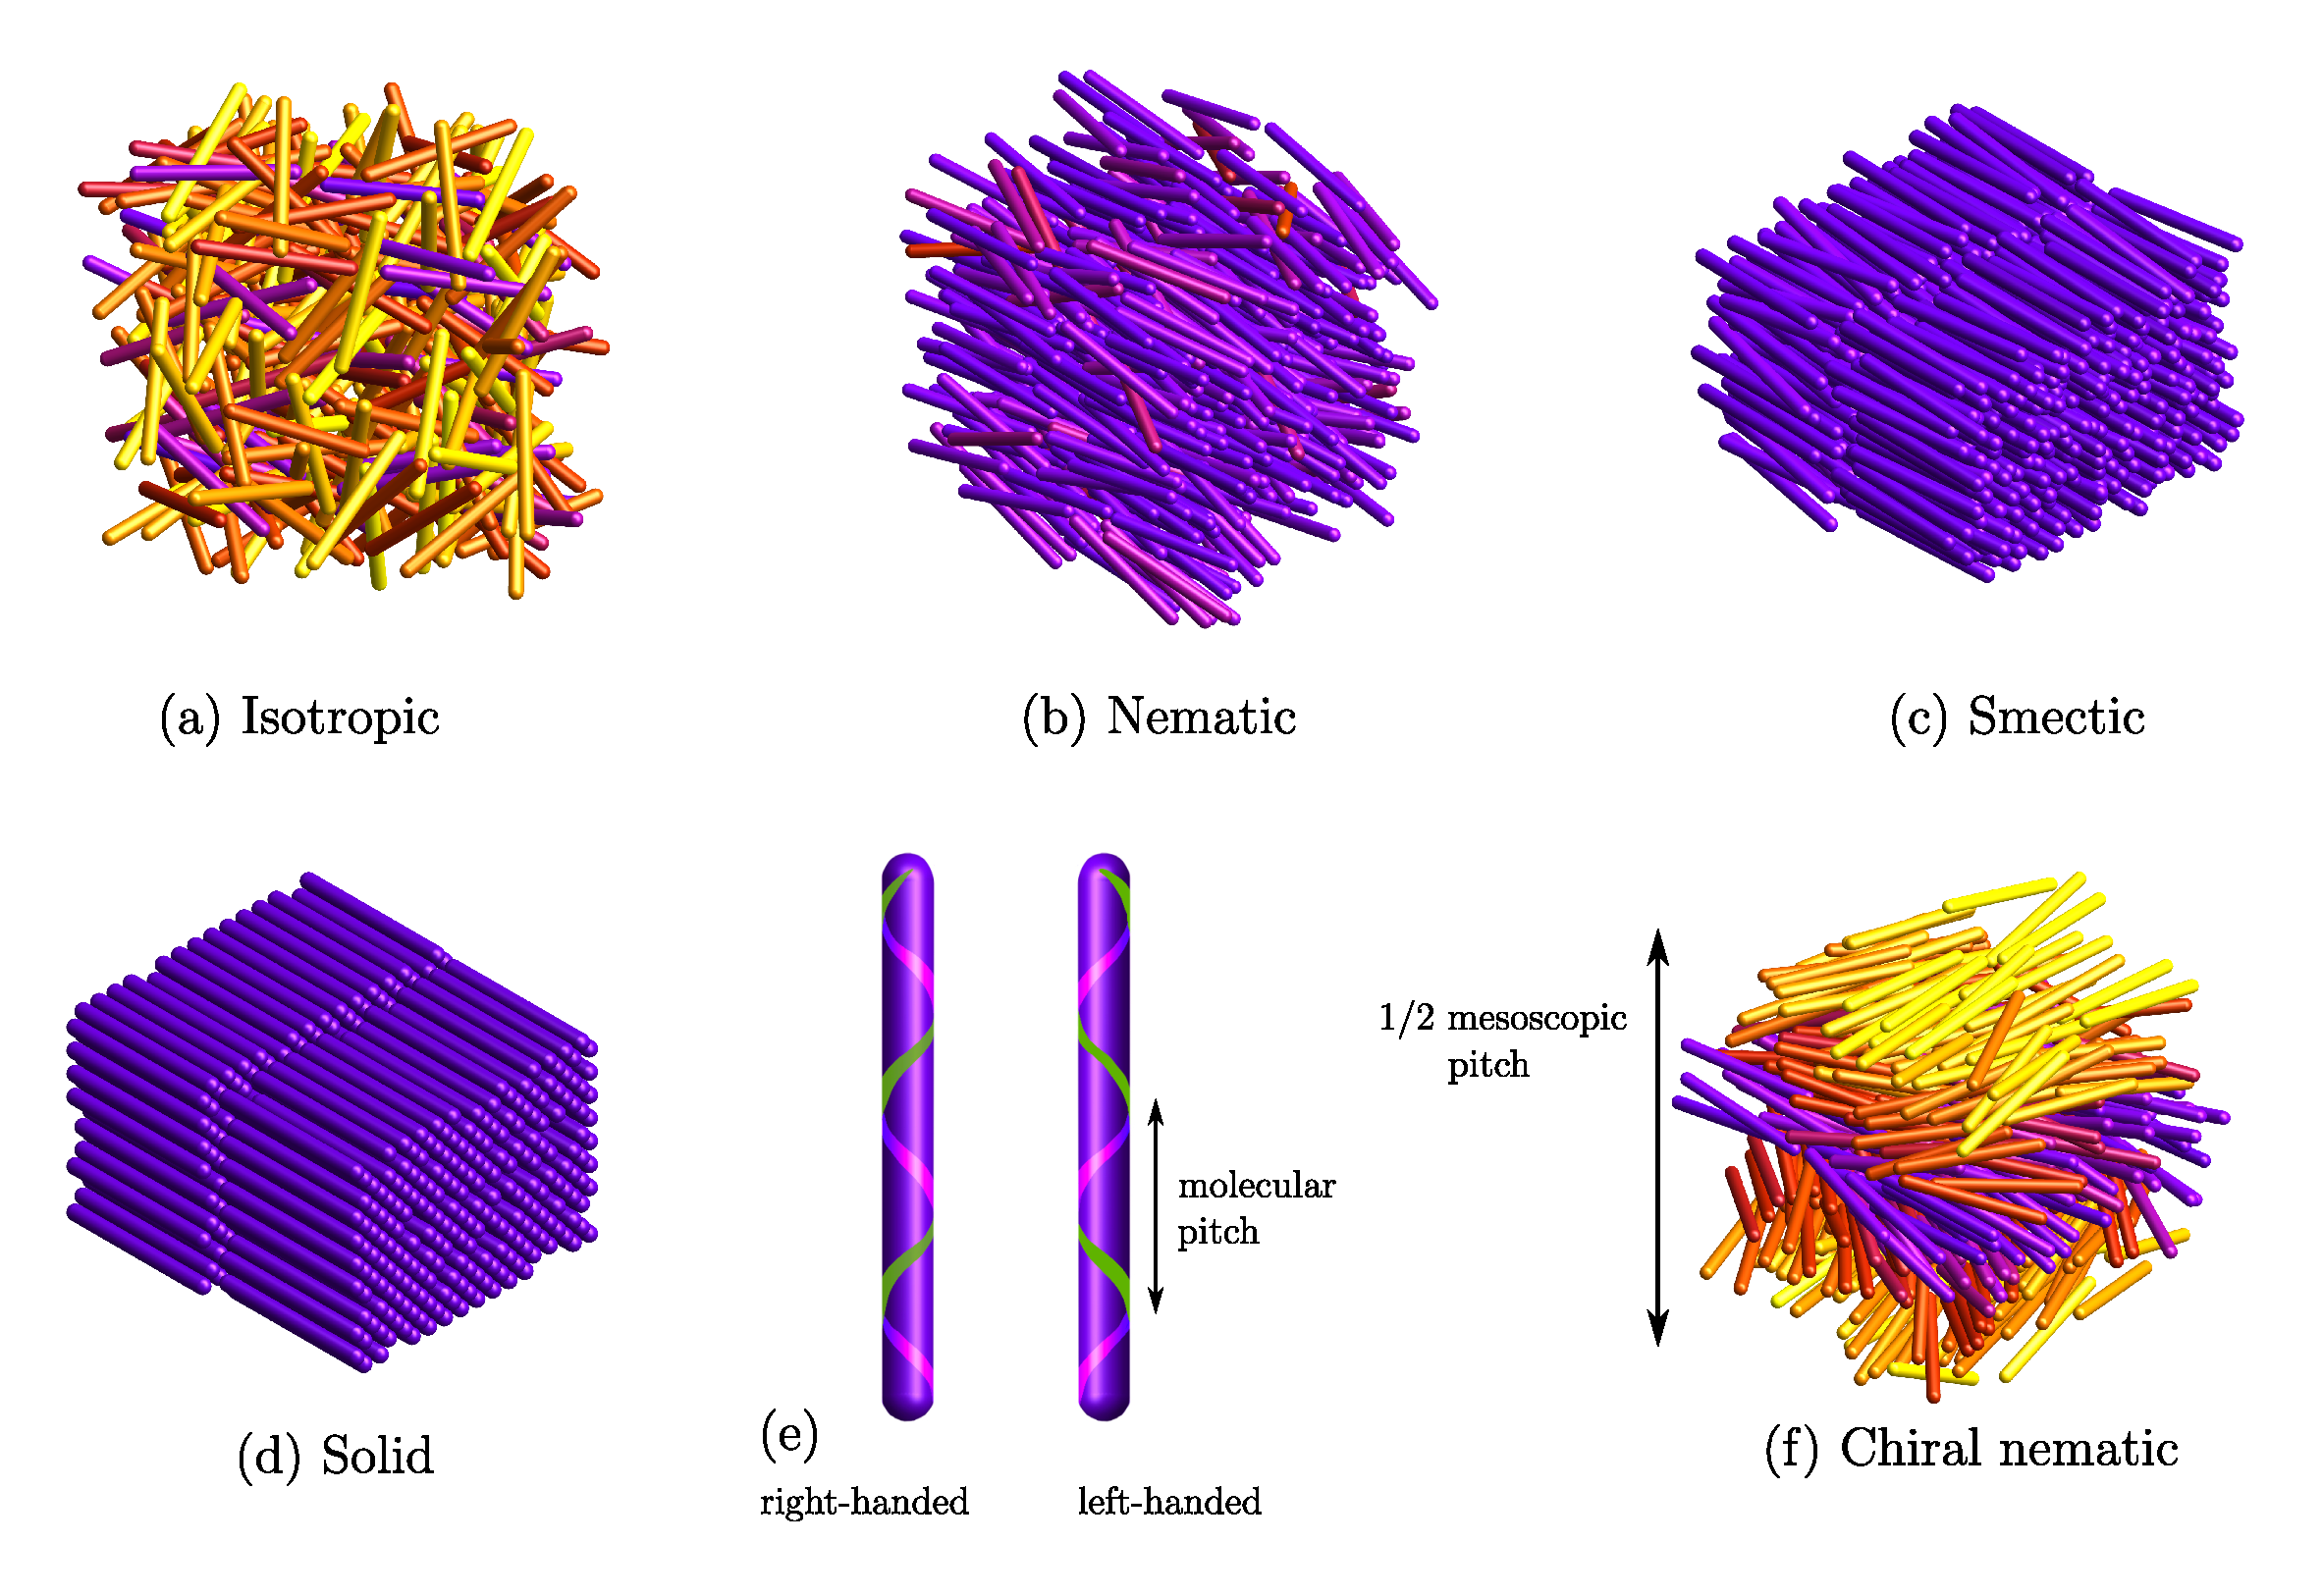
\includegraphics[width= \columnwidth]{figures/chapter-1/phases}
\caption{ \label{introfig1} (a)-(d) Examples of basic liquid crystals formed by rod-like molecules or nanoparticles. (e) Most molecular chiral features in elongated nano-particles  could be described on a coarse-grained level using a rod with an effective chiral electrostatic ``patchiness"  in terms of a molecular pitch length and handedness (left or right); (f) these particles generate a particular type of nematic phase: the chiral nematic. The implications of molecular chirality on the helical mesostructure (in particular, the mesoscopic pitch) of chiral nematic phases remains a challenging issue.}
\end{center}
\end{figure}

Among the numerous liquid crystalline phases, different degrees of order can be found, evidenced for instance by diffraction of X-rays and light. Measurements of this kind provide a frame to classify these systems by its similarity to either the gas or the solid phase. Let us consider, among others, the following liquid crystalline phases, depicted in \fig{introfig1}:

The {\em isotropic} (I) fluid phase is very similar to the gas and liquid phases for spherical particles and is characterized by a complete absence of positional and orientational order. At the inmediately next stage, we find the {\em nematic} (N) phase, in which particles are homogeneously distributed without positional order as in a liquid phase, but are ordered in their orientation following an average direction: the {\em nematic director} $\bn$. As it will be repeatedly discussed throughout this thesis, in nature one can find particles that, in addition to being anisotropic, present chiral features. This can be due to the arrangement of atoms in a molecular compound, to a (helicoidal) particle shape in some colloidal systems or to a chiral distribution of charges at the surface of the particles, observed for instance in {\em fd} filamentous bacteriophages viral rods \cite{Gibaud_2017}. When chiral particles are in nematic phase, they arrange themselves into a strongly twisted structure. This special case of a nematic phase is often called {\em cholesteric}.

The {\em smectic} (Sm) phase is closer to the solid phase. In smectic liquid crystals, particles are ordered in layers and cannot move freely between them. The smectic phase is, in turn, divided into several sub-phases with slightly different properties. Examples are the smectic A phase (SmA), where particles can move freely inside the layers as in a two-dimensional liquid; or the smectic B phase (SmB), where there is long-ranged positional order: at higher concentrations or lower temperatures, molecules tend to arrange themselves into something more similar to a crystalline lattice.

One sub-classification of liquid crystal materials is based on the mechanism by which they transition from one state to another. {\em Thermotropic} systems, mainly formed by low molecular weight constituents --and also some polymers--, undergo phase transitions due to changes in temperature, since the thermodynamic properties of these species depend on the attractive forces between the molecules. In this thesis, we focus mostly on  {\em lyotropic} liquid crystals, which form upon increasing the concentration of solute particles. This is the case of systems formed by high-molecular weight synthetic and biological nano-particles \cite{sonin1998inorganic,dogic-fraden_fil}, polymers such as DNA \cite{livolantDNAoverview} or surfactants in a solvent \cite{fontell1981}. The first case is the one studied in this thesis, where the fact that shape is not subject to fluctuations due to changes in the solvent composition is an advantageous simplification with respect to its amphiphilic and polymeric counterparts.

First experimental reports of nano-particle based lyotropic liquid crystals go back when liquid crystalline behaviour was described for tobacco and tomato mosaic virus (TMV) \cite{Bawden,Bernal} and vanadium pentoxide (V$_{2}$O$_{5}$) \cite{Zocher} in the early 20th century. In addition to these rod-like particle systems, colloidal plate-like charged particles and clay particles were discovered to report liquid crystalline behaviour \cite{Langmuir}. At present, there are many other examples of lyotropic liquid crystals to be found in a wide variety of dispersions of (mainly rod-like) colloidal particles and solutions of stiff polymers (see e.g. \cite{Dierking2020} for an overview).

This research work focuses on both theoretical and numerical approaches for the exploration of phase behavior in anisotropic colloidal compounds, with a particular interest in the {\em entropic} isotropic-nematic phase transition. This transition is well described by Onsager's theory, proposed in 1949, which assumes a similarity between a gas and a particle solution \cite{onsager1949}; and will be used repeatedly throughout this manuscript (more specifically in Chapters \ref{disc_polymer} and \ref{hybridLC2}) along with other theoretical and numerical tools to study the liquid-crystalline self-organization of colloidal rods or platelets in complex environments. Through our research, we hope to gain a better understanding of the behavior of this kind of systems and contribute to the broader field of liquid crystal research.

\subsection{Entropic phase transitions}
\label{entropy_order}

The thermodynamic equilibrium state of a system tends to minimize its Helmholtz free energy:

\beq
F=U-TS
\label{genhelmholtz}
\eeq
where $U = \sum_{i \neq j} u_{ij}$ is the internal energy of the system defined as a pairwise addition of interparticle potentials $u_{ij}$ between particles $i$ and $j$, $T$ is the temperature and $S$ is the entropy of the system. Clearly, a system at constant temperature can lower its free energy in two ways: either by increasing the entropy or by decreasing the internal energy. Entropy is defined, for an isolated system of $N$ particles in a volume $V$ at an energy $U$, as follows:

\beq
S = k_B\log(\mbox{\# {\small accessible states}})
\eeq
and depends on the total number of states that are accessible to the system under these conditions. Usually, $S$ is interpreted as a measure for the ‘disorder’ in that system. The natural consequence of this interpretation would be that ordering phase transitions can only take place if the loss in entropy is compensated by the decrease in internal energy. These kind of phase transitions are known as {\em energetic} phase transitions and describe the reality, for example, of the spontaneous phase transition from the regular fluid to the solid crystalline state. In this case, the transition takes place if the freezing lowers the internal energy of the system sufficiently to offset the decrease in the number of accessible configurations and thus the loss in entropy.

However, we can have many ‘ordering’ transitions that are {\em entropic}. Taking \eq{genhelmholtz} one may consider systems in which the internal energy is a function of temperature alone, $S$ being the only quantity affected by any change in the system at constant temperature. If this is the case, it will be possible to find phase transformations determined exclusively by a change in the entropy. Usually, atomic systems do not fulfill this condition because of the existence of attractive or repulsive interactions $u_{ij}$ whose strength depends on the relative inter-particle distance, an thus, the number density of particles $\rho$ when considering the thermodynamic limit. Temperature is then key to determine the accessibility of an ordered state, following the Boltzmann probability of finding a particle configuration of energy U, $\exp( -U/k_{B}T)$. Nevertheless, if we limit our attention to hard-core potentials:

\beq
V(r)=
\begin{cases}
\infty & r<D \textrm{ (if cores overlap)}\\
0 & r>D \textrm{ (if cores do not overlap)}
\end{cases}
\eeq
where $D$ is the diameter of the hard-core shell (which becomes an orientation-dependent quantity for anisotropic particles) and $r$ is the distance between centres of mass, then all the allowed (non-overlapping) configurations at constant temperature will possess the same level of internal energy $U=0$. Interestingly, $T$ then becomes completely irrelevant and any variation in the Helmholtz free energy will be attributed to changes in entropy, that will be maximized at equilibrium. Ordering phase transitions may occur in systems of this kind, e.g. in systems formed by rod-like particles, considering that entropy in these systems can be partitioned into two different components:

\beq
S = S_{trans} + S_{rot}
\eeq
where $S_{trans}$ is the translational entropy, related to accessible arrangements due to translational degrees of freedom and $S_{rot}$ is associated with the ways in which the particles can orient or rotate. The notion that spontaneous ordering of particles corresponds to an increase of the total entropy can be understood under this frame as a competition between these two quantities. When some kind of order emerges, particles lose entropy because the density --in terms of orientations-- is no longer uniform. However, this loss is more than offset by the simultaneous gain of translational entropy, i.e.  the available space per particle increases as the particles align. This argument can be extended to higher density phase transformations where positional order is achieved and the available volume each particle is allowed to explore increases if particles are arranged in a more ordered state instead of keeping a homogeneous positional distribution.

The isotropic-nematic phase transition invoked above occurs through a first order transition, as it was probed theoretically by Onsager. He recognized that the transition from an isotropic to a nematic state in solutions containing sufficiently anisometric particles can be described successfully  within a virial expansion of the free energy truncated after the second virial term, an approach which could not be used to explain the gas-liquid transition for spherical particles. About a decade after Onsager's work, Alder Wainwright and others \cite{ALDER57,WOOD57} first showed by means of computer simulations that a similar disorder-order transition, albeit of the positional degrees of freedom, occurs in a fluid of hard spheres, where there is a critical packing fraction at which particles will be able to better explore the translational phase space by adopting an (fcc) lattice rather than a disordered arrangement. Much later, computer simulations by Frenkel {\em et al.}  revealed the stability of smectic and columnar liquid crystals which appear upon densifying systems of respectively hard rods \cite{Frenkel88} and hard platelets \cite{FrenkelLiqcryst,Veerman},  without  attractive interactions between the particles. All of them consist of transitions driven entirely by {\em entropic} interactions.




\subsection{Mixtures and the depletion effect}

So far we have implicitly assumed that all particles which build up a gas, liquid (crystal) or solid phase are identical. Many systems in nature are however {\em mixtures} containing a number of different types of particles or molecules. It is not surprising that the phase behaviour of mixtures is richer than that of pure systems--if only for the additional {\em entropy of mixing}-- and that mixing different species may lead to  phenomena not encountered in one-component systems. An example of a purely entropically-driven self-assembly phenomenon is the ordered arrangement that arises in colloidal mixtures of large particles and smaller particles called depletants, a process known as the depletion effect.

\begin{SCfigure}
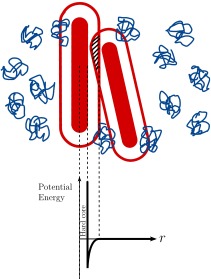
\includegraphics[width= 0.4 \columnwidth]{figures/chapter-1/depletion}
\caption{ \label{introfig2} The presence of non-adsorbing polymers or other depletions agents (whose size is usually smaller than the colloidal nanoparticles) produces an effective attractive potential between the rods according to the depletion scenario --which depends on the rods relative orientation and distance--. If the rods are at close proximity, the polymers are depleted away from the inner space between the rods in dictated by the overlap of the depletion zones (hatched area). This creates an osmotic imbalance around the cylindrical surfaces pushing the rods together.  }
\end{SCfigure}

This effect takes place typlically when colloidal particles are mixed with non-adsorbing polymers. \fig{introfig2} highlights the ordering transition in this situation by illustrating the effective attractive interaction between large colloidal rods when polymers are added to the system. Negative adsorption results in a region near the colloidal surface, named {\em depletion layer}, where polymers are less likely to access due to a loss of configurational entropy of the polymer chain. When such regions overlap, there is an increase in the volume available to polymers to explore, thus increasing their entropy and lowering their Helmholtz free energy. Effectively, the addition of depletants to the system generates repulsion between particles of distinct type and, in consequence, attraction between similarly-shaped colloidal particles.

These polymers are often modeled as penetrable hard spheres, known as Asakura-Oosawa spheres, in honor of the first theoreticians who proposed a model to describe the depletion effect \cite{ASAKURA54,ASAKURA58,Vrijdepletie}. By replacing the polymers with spheres of the same radius of gyration, we can obtain the same results in an effective manner. Penetrable hard objects do not interact with each other, i.e. no overlap restrictions are imposed between them, allowing for an ideal gas statistical mechanical treatment; and at the same time they are not allowed to overlap with colloidal particles, causing the emergence of the depletion effect. To sum up, the main approximations assumed by Asakura and Oosawa are: 1) whereas polymer chains in reality are unlikely found inside the depletion layers, in this model they are strictly prohibited; and 2) polymer chains are assumed to be completely transparent to each other, which is a fair approximation in the low depletant concentration regime.

In this work, depletion-driven demixing caused by strong shape assymetry in colloidal mixtures emerges in a natural way in Chapter \ref{disc_polymer} for a system featuring discs and polymerizing rods. In addition to it, the consequences of using penetrable hard spheres as a driving agent to stabilize liquid crystalline droplets will be deeply explored in Chapter \ref{twistedrods}.

\section{Scope of this thesis}

The central aim of this thesis is to theoretically investigate the liquid crystal (LC) self-organization of colloidal particles with different shapes in various contexts. Many of the studies to be described in the remainder of this thesis have been inspired by recent experimental works in systems of colloids with well-controlled shapes and interactions. In particular, we mention the experimental work of \cite{Grelet2014} on phase behavior and functionalization of complex fluids of filamentous bacteriophages (fd and M13) which display many interesting phenomena left open for theoretical interpretation; as well as recent experimental findings \cite{senyuk2021nematoelasticity,mundoor2021} on colloidal dispersion of highly anisotropic particles immersed in molecular LC hosts. One of our primary goals in this work is to account for these experimental observations by constructing simple, yet realistic,  models for the colloidal systems under consideration and by scrutinizing relevant aspects of their phase behaviour.

Chapter \ref{introduction} of this thesis provides an introduction to the background and scope of the research presented. It covers the statistical mechanical background, specifically for fluids of hard anisometric particles. We then discuss the use of hard particle Monte Carlo simulations of colloidal nematics, including some particularities of such simulations for the case of anisometric particles. Overall, the chapter serves as a foundation for the rest of the thesis, laying out the relevant concepts and methods for the research presented in subsequent chapters.

In Chapter \ref{disc_polymer} a simple model is proposed to explore the low-concentration phase behavior of a system consisting of non-covalently bonded, weakly flexible rods treated as living polymers mixed with non-adsorbing rigid colloidal discs. We show that, at large disc mole fractions, the rod nematic phase is disrupted by collective disc alignment in favor of a discotic nematic fluid in which the polymers are dispersed anti-nematically, generating a non-exponential molecular-weight distribution of the resulting polymeric species.

Chapters \ref{hybridLC1} and \ref{hybridLC2} address issues related to hybrid molecular liquid crystal nematics. In this part of the work, we consider a system in which molecular cholesteric LCs are doped with thin colloidal particles with large length-to-width aspect ratios. In Chapter \ref{hybridLC1}, single colloid insertions are considered, and we explore the interplay between weak surface anchoring forces, exerced between the colloidal surface and the molecular field, and elastic distortions around the colloid-molecular field interface. In Chapter \ref{hybridLC2}, we use Onsager's theory to account for collective effects in the hypothetical case where multiple colloidal particles are inserted in the hybrid LC.

Finally, in Chapter  \ref{twistedrods} we introduce a computational model to simulate mesoscopic droplets of colloidal rods stabilized by the presence of non-adsorbing polymers. We aim to gain a deeper understanding of the transition between the so-called twisted membranes and twisted ribbons observed experimentally in systems featuring filamentous fd viral rods \cite{Gibaud2012} by performing Monte Carlo simulations in the semi-grand-canonical ensemble. Although twisted ribbons are not observed in our simulations, a theoretical model is proposed to predict the typical ribon geometric features that can in principle be confirmed through experimental verification.


\section{Statistical mechanical background}

In this section we introduce the statistical mechanical framework of  Onsager's second virial theory to describe the thermodynamic properties of a spatially homogeneous fluid of hard colloidal rods or platelets. Instead of delving into a technical exposition of Onsager's theory (the reader is referred to Onsager's original paper \cite{onsager1949}, as well as some enlightening reviews \cite{Vroege92, allenevans} for more detailed information), we will provide an intuitive overview of its main components. As explained in Section \ref{entropy_order}, the isotropic-nematic phase transformation result from the competition between two principal quantities, related to rotational and translational degrees of freedom. Onsager establishes the formulation of these two quantities and analyzes the transition unsing entropic arguments alone.

\subsection{Fluids of hard anisometric particles}

Let us assume an ensemble of slender rigid needles in a fluid state of uniform particle density $\rho = N/V$ at a fixed volume $V$ and temperature $T$, and focus on the orientational phase space the rods adopt in a fully isotropic and nematic configuration. If we treat each rod orientation on the unit sphere as a separate state we may define an orientational entropy as the ratio of the number of explorable orientational states:
\begin{equation}
\frac{S_{or}}{N} \sim k_{B} \ln ( \mbox{\# {\small orientational states}})
\label{sor}
\end{equation}

More specifically, the following expression for the orientational free energy can be obtained:

\begin{equation}
\frac{S_{\text{or}}}{N}=-k_B\int f(\Omega)\ln \left[4\pi f(\Omega)\right]d\Omega.
\label{0forient}
\end{equation}
where $f(\Omega)$ is the normalized {\em orientational distribution function} (ODF) that in general depends on a solid angle $\Omega$. This expression is derived by applying the following assumptions:

\vspace{0.3cm}
\begin{enumerate}
\setlength\itemsep{1em}
\item Start from the configurational partition function for an imperfect gas where the total potential energy is expressed as a summation over particle pairwise interactions that are orientation dependent.
\item Assume the analogy between an imperfect gas and a dispersion of colloidal particles in a solvent with fixed chemical potential.
\item Divide the orientational space into $s$ arbitrarily small solid angle sections, consider each rod orientation as a separate species and transform the partition function to account for a mixture of $s$ species, each one of $N_k$ particles with $k = 1,\ldots,s$, such that
\begin{equation}
\sum _{k=1}^{s} N_{k} =N. \label{0behoud}
\end{equation}

\item The partition function then becomes a complicated summation over all possible combinations of $\{N_{1},N_{2}, \ldots, N_{s}\}$ satisfying \eq{0behoud}. For large $N$, however, it is justified to approximate the complete set of summations by its maximum term. Let us define $\{\tilde{N}_{1},\tilde{N}_{2},\ldots,\tilde{N}_{s}\}$ as the orientation distribution associated to the maximum term of the summation.
\item After some rearranging, the following expression can be obtained for the orientational part of the free energy:
\begin{equation}
\beta F_{\text{or}}=N\left\{\ln \left[\frac{4\pi}{\Delta \Omega}\right] + \sum_{k=1}^{s}\frac{\tilde{N}_{k}}{N}\ln \frac{\tilde{N}_{k}}{N} \right\},
\label{0fordiscreet}
\end{equation}
where $\beta=1/k_BT$ $\Delta \Omega = 4\pi/s$ is the chosen size of the angular bins.

\item Taking the limit $\Delta \Omega \rightarrow 0$ for a {\em continuous} distribution in $\Omega$ we directly obtain \eq{0forient}.
\end{enumerate}
\vspace{0.3cm}

It is clear, following \eq{0forient}, that the orientational entropy is maximized when the ODF is isotropic. In consequence, and since in a nematic phase the needles are strongly aligned along either poles of the unit sphere, we infer that the orientational entropy of a nematic phase is always smaller than that of an insotropic fluid at comparable particle orientation.

Let us focus now on the other competing part of the entropy in this system. The translational free energy of an ensemble of slender rigid needles can be approximated systematically by a virial expansion in terms of the density $\rho=N/V$ \cite{hansenmacdonald}. Starting from the law of ideal gases applied to a colloidal solution:

\begin{equation}
\Pi V = N k_B T
\end{equation}
where $\Pi$ is the osmotic pressure of the system, the virial correction can be applied as follows:
\begin{equation}
\beta \Pi = \rho + B_2\rho^2 + B_3\rho^3 + \ldots
\end{equation}
where $B_2$ and $B_3$ are the second and third virial coefficients, and are calculated by integrating simultaneous interactions between two and three particles respectively:

\begin{equation}
B_2 = -\frac{1}{2V} \int \int \Phi_{12} d {\bf r}_1 d {\bf r}_2
 \label{B2}
\end{equation}
\begin{equation}
B_3 = -\frac{1}{3V} \int \int \int \Phi_{12} \Phi_{13} \Phi_{23} d {\bf r}_1 d {\bf r}_2 d {\bf r}_3
\end{equation}
where $\Phi_{ij} = \exp(-u_{ij}/k_BT)-1$ are the so-called Mayer functions. Onsager stated by geometrical arguments that the following scaling relation for $B_2$ and $B_3$ is fair for long thin rods:
\begin{equation}
\frac{B_3}{(B_2)^2} \sim \frac{D}{L}\left ( \ln \frac{L}{D} + cst. \right )
\end{equation}
which vanish in the limit of infinitely thin needles. The decrease  has been  verified by means of Monte-Carlo simulations on hard spherocylinders by Frenkel \cite{Frenkel87,Frenkel87err} showing that higher order virial coefficients can be neglected only if $L/D\gg 100$. The situation is much different for thin platelets for which Onsager estimated

\begin{equation}
\frac{\beta_{2}}{\beta_{1}^{2}}\sim \mathcal{O}(1), \label{0clusterplate}
\end{equation}
which is also true for spheres. Therefore, virial contributions of order higher than two can be neglected for thin needles, which allows for a simplified analytical treatment of the problem in contrast to the case of non-elongated particles where higher orders must be considered. These higher order contributions in the virial expansion --involving clusters of three, four, etcetera particles-- can be derived using other methods, albeit approximately, such as `scaled particle' \cite{Cotterspt,Cotter} and density functional theories (see \cite{Vroege92,DFTspecialJPCM} for a review). In this thesis, due to the low density regime regarded in all the analytical works, it is reasonable to stick to the second virial approximation.

What remains now is to integrate the second virial coefficient. For the system presented here, the pairwise interaction between particles $u_{ij}$ is strictly hard and depends on the relative orientation between needles; we can thus deduce
\begin{equation}
\Phi_{ij}=\Phi(\Omega_1,\Omega_2)=
\begin{cases}
-1 & \textrm{if overlap}\\
0 & \textrm{otherwise}
\end{cases}
\end{equation}

The interaction between two particles only contributes to the integral in \eq{B2} if particles are close enough to overlap, i. e. if they are both contained inside the {\em excluded volume} generated from their relative orientations:

\begin{equation}
B_2 = \frac{1}{2} \int \int v_{excl}(\Omega_1,\Omega_2) f(\Omega_1) f(\Omega_2)\frac{d\Omega_1}{4\pi}  \frac{d\Omega_2}{4\pi}
 \label{B2_exclv}
\end{equation}

\begin{SCfigure}
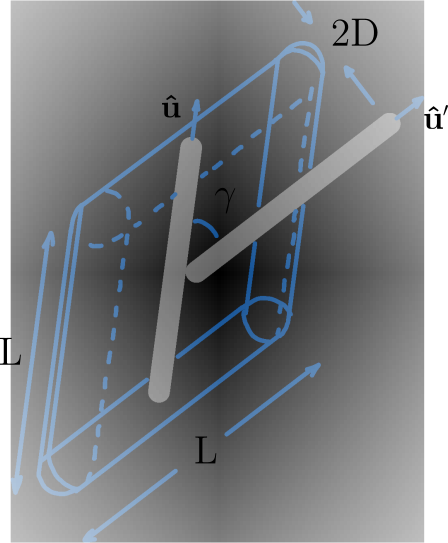
\includegraphics[width= 0.4 \columnwidth]{figures/chapter-1/exclvol}
\caption{ \label{introfig3} Illustration of the excluded volume of two spherocyllinders  of length $L$ and diameter $D$ at mutual orientation $\gamma$. Rod alignment leads to a strong reduction of the excluded volume represented by the lozenge-shaped figure.}
\end{SCfigure}

Since we are accounting for possible inhomogeneous angular configurations, the previous reformulation of the integral must be weighted by the ODF $f(\Omega)$.

The meaning of the excluded volume is clarified in \fig{introfig3}. Considering long hard rods we immediately infer that the excluded volume is strongly orientation-dependent; it is greatly reduced when the rods align. In consequence, taking \eq{B2_exclv} one can see that collective alignment of the rods and thus an anisotropic ODF will reduce the value of $B_2$ with respect to an isotropic state.

Lastly, we recall the free energy formulation of an imperfect gas approximated by the second virial correction:
\begin{align}
\frac{\beta F}{N} =& \beta \mu_{0}+\ln\left[\Lambda\rho\right]-1+ B_2 \rho
\end{align}
with $\mu_{0}$ a reference chemical potential of the dispersed particles depending only on the solvent conditions, and $\Lambda$ the (de Broglie) thermal volume, arising from
integrations over the translational and rotational momenta of the anisometric particles. The last term corresponds to the translational {\em entropy} in the context of Onsager's formalism, since for hard core interactions it does not depend on temperature, but only on the average over all possible configurations. Collecting the previous results from \eq{0forient} and \eq{B2_exclv} we obtain the following expression:
\begin{align}
\frac{\beta F}{N} =& \beta \mu_{0}+\ln\left[\Lambda\rho\right]-1+
\int f(\Omega)\ln \left[4\pi f(\Omega)\right]d\Omega \nonumber \\
&+\frac{\rho}{2} \iint d\Omega d\Omega^{\prime}
f(\Omega)f(\Omega^{\prime})v_{\text{excl}}(\Omega,\Omega^{\prime}). \label{0freetot}
\end{align}

This is the final recipe to model the phase behavior of an ideal mixture of hard rods, where the most probable orientational state is given by the function $f(\Omega)$ that better minimizes the Helmholtz free energy. The isotropic-nematic transition comes from a competition between the before-last and last terms, which correspond to the orientational and translational entropy respectively. For low concentrations, the orientational entropy dominates and is maximized by an isotropic distribution, whereas for high concentrations the second virial term becomes more important, which favors a nematic distribution at the expense of losing orientational entropy. The critical packing fraction at wich an isotropic-nematic ordering occurs roughly corresponds to the situation when the bare particle volume is of the same order of magnitude as its average excluded volume:

\begin{equation}
\phi_{IN} \propto \frac{\mbox{{\small volume per particle}}}{\mbox{{\small average excluded volume per particle}}}
\end{equation}

The excluded volume for a pair of spherocylinders as sketched in \fig{introfig3} reads

\begin{equation}
v_{excl}(\Omega_1,\Omega_2) = 2L^2D |\sin\gamma|+2\pi D^2 L + \frac{4}{3}\pi D^3
\end{equation}

An analogous expression was obtained by Onsager for two cylinders with different arbitrary lengths, diameters and mutual orientation \cite{onsager1949}. Simple scaling considerations for thin cylinders then prompt us to infer that, whereas the volume per particle scales as $\propto L D^2$, the excuded volume typically goes as $\propto D L^2$. In consequence,


\begin{equation}
\phi_{IN} \propto \frac{D}{L}
\end{equation}

Clearly, the more slender the rods (large $L/D$) the lower the critical packing fraction at which the I-N phase transformation can be expected. Strictly, in the Onsager limit $L/D \rightarrow \infty$ the transition occurs in the ultra-dilute regime where a pair-interaction-only approximation is entirely justified.

\subsubsection{Mixtures}

Chapter \ref{disc_polymer} will focus on mixtures of anisometric particles consisting of multiple distinct species (e.g., mixtures of discs and polymers with multiple aggregation numbers). Introducing mole fractions $x_{j}=N_{j}/N$ for each species $j$, the free energy of the mixture can be expressed as a straightforward generalization of \eq{0freetot}:

\begin{align}
\frac{\beta F}{N} &\sim \ln [\rho \bar{\Lambda}]-1 + \sum_{j} x_{j} \ln x_{j} +
\sum_{j} x_{j} \int f_{j}(\Omega)\ln \left[ 4 \pi f_{j}(\Omega) \right] d \Omega \nonumber \\
&+\frac{\rho}{2}\sum_{j}\sum_{k}x_{j}x_{k} \iint  d \Omega d\Omega^{\prime}
f_{j}(\Omega)f_{k}(\Omega^{\prime})
v_{\text{excl}}^{jk}(\Omega,\Omega^{\prime}),  \label{0freetotmulti}
\end{align}
with $\bar{\Lambda}=\prod_{j}\Lambda_{j}^{x_{j}}$. The contribution $\sum_{j} x_{j} \ln x_{j}$ represents the {\em entropy of mixing} due to the fact that we are dealing with different species. Although the free energy for mixtures can be easily established,  the implications of \eq{0freetotmulti} are quite significant. In particular, each species $j$ now has its own ODF which must be normalized according to $\int f_{j}(d\Omega)d\Omega \equiv 1$. Moreover, in the case of phase coexistence between an isotropic ($I$) and a nematic ($N$) phase, the conditions for mechanical and chemical equilibrium require equal osmotic pressure $\Pi$ and chemical potentials $\mu_{j}$ for {\em all} species involved. Thus, the coexistence equations read:

\begin{align}
\Pi^{I}&=\Pi^{N} \nonumber \\
\mu^{I}_{j}&=\mu^{N}_{j} \qquad\qquad \text{for {\em all} $j$},
\end{align}

where we must take into account that the composition ${x_{j}}$ may differ in each phase due to fractionation effects. These considerations indicate that the calculation of phase transitions in mixtures is generally a challenging task, requiring specific approximations or numerical techniques depending on the physical situation. More details on the particular approaches addressed in this research work can be found in Chapter \ref{disc_polymer}.

\subsection{Facing reality}

Going back to the experimental systems of nanorods and platelets mentioned at the beginning of this chapter it is clear that a simple hard-particle model is often too simple to arrive at a satisfactory description of a typical experimental setup. A number of extensions and modifications of Onsager's theory are then necessary. Some of them involve attempts to account for:

\begin{enumerate}
\item Multicomponent mixtures of rod, disks, or living polymers
\item Effect of external aligning fields
\item Semi-flexibility
\item Long-ranged ``soft" interactions (e.g. depletion attraction)
\item Chirality
\item Non-uniform systems (smectic membranes, interfaces, effect of solid substrates)
\end{enumerate}

In the main body of this work we will illustrate the rich phenomenology brought about by the topics listed above, most of the time as perturbations to the main entropic hard-core contribution, discussed previously in the context of Onsager's theory. We hope that these examples will convince the reader of the predictive power and versatility of Onsager's second-virial theory even when applied beyond the strict bounds of applicability as formulated in his original paper. In what follows, topics 4 and 5, albeit already introduced, are now very briefly discussed from a more quantitative perspective.

\subsubsection{Depletion}

Similar to a Yukawa potential, while the depletion interaction remains relatively tractable for simple spherical particles, the quantity becomes highly non-trivial for more complex colloidal shapes. This is due to the intrinsic orientation-dependence of the depletion zones and their overlap conditions when generalized to suspensions involving rod or disk-shaped nanoparticles, and also to the non-additive nature of the depletion potential when the size of the depletants is comparable to the width of the colloids. The depletion attraction between non-isotropic particles could be formally expressed as a mean-field correction term:


 \begin{equation}
U \sim  -\frac{1}{2} \frac{N^{2}}{V} \Pi_{dep} \left \langle \int_{
\substack{
\mbox{\tiny no core overlap,} \\
\mbox{\tiny depletion zone overlap}
}
} d {\bf r}_{ij}   v^{dep}_{ij}({\bf r}_{ij})  \right \rangle_{\mbox{\tiny orientational states of rods i and j}}
\label{degen}
\end{equation}
where $\Pi_{dep}$ is the osmotic pressure of the depletants. In arriving at this expression, the depletion agents have been considered to be mutually non-interacting and the effective attraction ptential between the nanoparticles is proportional to the overlap volume $v^{dep}_{ij}$ of the depletion zones of particles $i$ and $j$ (see \fig{introfig2}) \cite{LekkerkerkerTuinier2011}.

\subsubsection{Chirality}

The presence of surface charges (or {\em soft patches}) residing on the colloid surface in a distinctly {\em helical} distribution can impart a distinctly chiral signature on to the effective interactions between the nanoparticles. In this case, there is a supplementary soft interaction coupling to the rod orientation vector $\bhu$ of each rod $i$ and $j$ (see \fig{introfig1} (e) and (f)) and their centre-of-mass distance vector $\bf r$ through the following pseudo-scalar expression \cite{goossens1971}:
\beq
u_{ij} \sim  \varepsilon_{c} g( r)({\bf \hat{u}}_{i} \cdot {\bf \hat{u}}_{j}) ( {\bf \hat{u}}_{i} \times {\bf \hat{u}}_{j} \cdot {\bf r} )
\label{chirality}
\eeq

In Chapter \ref{twistedrods}, we will analyze in detail the implications of this interaction for the chiral features of colloidal mesoscopic compounds, whose microscopic details can be encapsulated into the effective chiral amplitude $\varepsilon_c$ and decay function $g(r)$, which express the typical range over which chiral forces are transmitted. The effective potential is distinctly chiral and lacks inversion symmetry, meaning that it changes under a transformation ${\bf r}_{ij} \rightarrow -{\bf r}_{ij} $, while preserving basic head-tail symmetry $u_{ij}({\bf \hat{u}}_{i/j}) = u_{ij}(-{\bf \hat{u}}_{i/j}) $.

\section[HPMC simulations of colloidal nematics]{Hard-particle Monte Carlo simulations of colloidal nematics: some technical details}

In the last half century, the use of molecular simulations has become increasingly widespread across a multitude of scientific disciplines, representing an essential tool in the realm of colloidal and soft matter science. The initial success of these simulations can be traced back to their ability to predict the transition between the liquid and solid phases in a system of hard spheres \cite{ALDER57,WOOD57}. Since then, molecular simulations have become a pillar in soft matter research, allowing for the exploration of complex systems at the molecular level with remarkable accuracy and versatility.

Molecular simulations are classified into two principal categories: Molecular Dynamics (MD) and Monte Carlo (MC) simulations. The fundamental aim of both techniques is to acquire macroscopic observables from microscopic properties of the system. While MD simulations focus on time averages, MC simulations rely on ensemble averages. In the thermodynamic limit, these two types of averages become equivalent, according to the ergodic hypothesis, which postulates that a system traverses all possible states in its phase space over a long enough time scale \cite{dfrenkel96:mc}. As a result, the use of molecular simulations has led to significant advances in a variety of fields, ranging from materials science to biophysics and beyond, making them an indispensable tool for contemporary scientific research.

One of the advantages of MC over MD is that it permits to study systems characterized by non-analytical interaction potentials e. g. the hard core interaction invoked in this work. Using Monte Carlo simulations to explore the configurational space of a system at certain conditions, an observable $A$ can be calculated as an average over a big number of accessible configurations. In the canonical ensemble (systems at constant $\{N,V,T\}$) this can be integrated using the Boltzmann probability of finding a particle configuration of energy U, $\exp( -U/k_{B}T)$:

\beq
\langle  A \rangle = \frac{\int d \bfr^NA(\bfr^N)\exp(-\beta U)}{\int d \bfr^N\exp(-\beta U)}
\label{observable}
\eeq

A possible way to evaluate \eq{observable} is through the Metropolis Monte Carlo algorithm \cite{Metropolis1953}, which becomes much simpler for hard core systems due to the fact that, in this case, the Boltzmann factor can only be worth 0 or 1. The basic form of a MC cycle then becomes:


\begin{algorithm}[h]
    \SetAlgoLined

    Start from an initial configuration of $N$ particles\;
    \For{$k = 0,\dots,N-1$}{
        Choose a random particle $i$\;
        Give the particle a random transformation (translation or rotation)\;
        Check for overlaps\;
        \eIf{new configuration generates an overlap}{
            Reject: roll back to old configuration\;
        }{
            Accept: update the configuration\;
        }
    }
    \caption{Metropolis Monte Carlo algorithm for hard--core potentials in the canonical ensemble.}
    \label{algo:MHPMC}
\end{algorithm}


In this section we aim to give an overview of the technical peculiarities of Hard Particle Monte Carlo (HPMC) simulations of anisotropic particles, in particular mixtures of elongated rods and depletants, that are used in the computational model studied in Chapter \ref{twistedrods}.

\subsection{Overlap conditions for hard spherocyllinders}

As shown in Algorithm~\ref{algo:MHPMC}, in HPMC a move is accepted if there is no overlap between two particles. Hence an efficient overlap test is key in this technique. In the case of spherical objects the overlap test is very simple: it is enough to compute the distance between the center of the two spheres $r_{ij}$ and verify that it is less than the sum of their radii: $r_{ij} \leqslant R_i + R_j$ or, in a computationally cheaper form, $r_{ij}^2 \leqslant (R_i + R_j)^2$. It is possible to model elongated hard rods that use this simple overlap condition by building particles composed of spherical objects attached in a linear chain. In this case, the overlap test simply consists on evaluating pairs of spherical objects associated to distinct rods. However, the computational expense of this strategy is enormous as it involves the order of $N_b^2$ operations at each MC move where $N_b$ is the number of spherical beads in one rod.

This problem is overcome if each colloidal rod is considered to be a spherocylinder, for which a more efficient overlap test is proposed by Allen {\em et al.} \cite{allenevans93}. The key steps are outlined below.

A spherocylinder $i$ is defined by its cylindrical surface length $L$, the diameter $D$ of its cylindrical surface and its two hemispheres, the coordinates $\bfr_i$ of its center of mass and the unit vector $\bhu_i$ indicating its orientation. We want to determine the minimum distance between the cores of two spherocylinders $i$ and $j$ with equal lengths and diameters. We can describe any point of the line segment core of $i$ and $j$ parametrically as

\begin{align}
\bfr_i(\lambda) &= \bfr_i + \lambda \bhu_i \nonumber \\
\bfr_j(\mu) &= \bfr_j + \mu \bhu_j
\end{align}

In order to calculate the minimum distance between two arbitrarily oriented lines we can take advantage of the fact that the shortest distance vector,
\beq
\bfr_{ij}^{min}(\lambda_0,\mu_0)=\bfr_{j}(\mu_0)-\bfr_{i}(\lambda_0),
\eeq
must be perpendicular to both $\bhu_i$ and $\bhu_j$. Assuming $\bfr_{ij}^{min}(\lambda_0,\mu_0) \cdot \bhu_i = 0$ and $\bfr_{ij}^{min}(\lambda_0,\mu_0) \cdot \bhu_j = 0$ we obtain a system of equations that we can solve to get the minimizing values $\lambda_0$ and $\mu_0$:
\beq
\begin{pmatrix}
\lambda_0 \\
\mu_0
\end{pmatrix}
= \frac{1}{1-(\bhu_i \cdot \bhu_j)^2}
\begin{pmatrix}
-\bhu_i \cdot \bfr_{ij} + (\bhu_i \cdot \bhu_j)(\bhu_j \cdot \bfr_{ij}) \\
+\bhu_j \cdot \bfr_{ij} + (\bhu_i \cdot \bhu_j)(\bhu_i \cdot \bfr_{ij})
\end{pmatrix}
\label{overlapeq}
\eeq
where $\bfr_{ij} = \bfr_{j} - \bfr_{i}$ is the distance between centers of mass. Since for line segments $-\frac{L}{2} \leqslant (\lambda,\mu) \leqslant \frac{L}{2}$ we have to truncate the result of \eq{overlapeq} if it exceeds this limit. In order to avoid more arithmetical operations than necessary, at this point it is better to compute the square minimal distance
\begin{align}
(\bfr_{ij}^{min})^2(\lambda_0,\mu_0) = \bfr_{ij}^2& + \lambda_0^2 + \mu_0^2 - 2\lambda_0\bhu_i \cdot \bfr_{ij} \nonumber \\
    & + 2\mu_0\bhu_j \cdot \bfr_{ij}  - 2\lambda_0\mu_0\bhu_i \cdot \bhu_j
\end{align}
from quantities already calculated. All the above scheme works unless shperocylinders are completely parallel to each other, in which case \eq{overlapeq} is not well defined. We can add a condition to account for this particular case, where the minimal distance would be simply calculated as the distance between two parallel lines.

There is an overlap between the two spherocylinders if $(\bfr_{ij}^{min})^2 \leqslant D^2$. A generalization of this idea can be done for mixtures of two different species of spherocylinders of lengths $L_{1,2}$ and diameters $D_{1,2}$ by simply rewriting
\begin{align}
-\frac{L_i}{2}& \leqslant \lambda \leqslant \frac{L_i}{2} \nonumber \\
-\frac{L_j}{2}& \leqslant \mu \leqslant \frac{L_j}{2} \nonumber \\
    (\bfr_{ij}^{min})^2& \leqslant \left( \frac{D_i+D_j}{2}\right)^2
\end{align}
where $i,j=$ 1 or 2 if the spherocylinders belong to the first or second species respectively. For mixtures of spherocylinders and spheres, the expressions can also be valid by taking $L=0$ for spheres.

\subsection{Semi-grand canonical ensemble}

Several theories have been developed that enable calculations of phase transitions in systems with depletion interactions. The free volume theory (FVT) by Lekkerkerker {\em et al.} \cite{sphere+polymer} for the phase behavior of dispersions of colloids and non-adsorbing polymer was the first one to account for depletant partitioning over the coexisting phases. This theory is based on the osmotic equilibrium between two systems: a hypothetical depletant reservoir and a mixed colloid $+$ depletant system. Because of its affordability in terms of complexity and yet a phenomenologically accurate description of the problem, this theory serves as a standard reference today, both for theoretical and computational models.

The starting point is the {\em semi--grand} potential density of a system of colloids and polymer in equilibrium with a reservoir containing only the polymer. This semi--grand potential is separated into a hard colloid contribution and a polymer contribution. The colloid part may be described by known expressions for the colloidal fluid and crystalline phases in the canonical ensemble (fixed volume, temperature and number of colloidal particles $\{N,V,T\}$). The polymer contribution is found from a build-up principle: starting from a system without polymer, chains are added to the system until the final concentration is reached, and the polymer contribution is calculated by integrating along this path. This is the reason why the polymer part is treated in a more natural way by using the grand canonical formalism (fixed volume, temperature and polymer chemical potential $\{\mu_p,V,T\}$). The key assumption of this theory is that thermodynamic quantities can be calculated for both colloids and depletants from their independent ensembles, correlated only by means of an ensemble--averaged free volume for the depletants in the mixed system $\langle V_{free} \rangle$. As a result, we can define

\beq
\Omega(N,V,T,\mu_p) = F_0(N,V,T) - \Pi^R\langle V_{free} \rangle
\eeq
where $F_0$ is the free energy of the colloidal particle system without added depletant, $\mu_p$ represents the chemical potential of the polymer depletant and $\langle V_{free} \rangle$ is the available volume for the depletants, i.e. the total volume in the mixed system outside the depletion layers, and it is approximated by the free volume in the pure hard colloid dispersion $\langle V_{free} \rangle_0$. This approximation is valid in the limit of low depletant activity, and starts losing accuracy when increasing it. $\Pi^R$ is the osmotic pressure in the reservoir, and it can be easily calculated by considering the depletants as penetrable hard spheres, which allows for a real gas formulation and thus

\beq
\Pi^R=n_pk_BT
\eeq
where $n_p$ is the number density of the depletants in the reservoir. We can also write down the chemical potential:

\beq
\mu_p = \textrm{const} + k_BT\ln n_p
\eeq

In order to equate the depletant chemical potentials in both systems, we infer that the average number of depletants in the mixed system $N_p$ must fulfill
\beq
N_p= n_p\langle V_{free} \rangle
\eeq

In what matters to our simulations presented in Chapter \ref{twistedrods}, the total number of particles in a semi-grand MC scheme is no longer constant, but rather fluctuating towards an optimal value given by $N + N_p$. This allows us to stabilize mesoscopic colloidal compounds while maintaining a constant depletion pressure. Algorithm \ref{algo:MHPMC} is then rewritten as:

\begin{algorithm}[h]
    \SetAlgoLined

    Start from an initial configuration of $N$ colloids and $N_p$ depletants\;
    \For{$k = 0,\dots,N + N_p -1$}{
    Choose a random particle type\;
        \If{type is colloid}{
            Choose a random particle $i$\;
            Give the particle a random transformation (translation or rotation)\;
            Check for overlaps\;
            \eIf{new configuration generates an overlap}{
                Reject: roll back to old configuration\;
            }{
                Accept: update configuration\;
            }
        }
        \If{type is depletant}{
            Choose a random transformation (insertion or deletion)\;
            \If{insertion}{
                Generate random coordinates\;
                Check for overlaps\;
            \eIf{new configuration generates an overlap}{
                Reject: roll back to old configuration\;
            }{
                Insert with probability
                \beq
                    \sim \frac{V}{\Lambda(N_p+1)}e^{\beta\mu_p}\; \nonumber
                \eeq
            }

            }
            \If{deletion}{
                Choose a random particle $i$\;
                Delete with probability
            \beq
                \sim \frac{\Lambda N_p}{V}e^{-\beta\mu_p}\; \nonumber
            \eeq
            }
            Update $N_p$ if necessary\;
        }
    }
    \caption{Semi--grand canonical Monte Carlo scheme for mixtures of $N$ colloids $+$ depletants at constant chemical potential $\mu_p$. }
    \label{algo:semiHPMC}
\end{algorithm}




\subsection{Implicit depletants algorithm}

\clearpage % Introduction I: theoretical frame
\input{chapters/chapter-2} % Introduction II: MC simulations

\chapter{Mixtures of discs and reversible polymers}

\begin{abstract}
    Living polymers composed of non-covalently bonded  building blocks with weak backbone flexibility may self-assemble into thermoresponsive lyotropic liquid crystals. We demonstrate that the reversible polymer assembly and phase behavior  can be  controlled by the addition of (non-adsorbing) rigid colloidal discs which act as an entropic reorienting ``template"  onto the supramolecular polymers. Using a particle-based second-virial theory that correlates the various entropies associated with the polymers and discs, we demonstrate that small fractions of discotic additives promote the formation of a polymer nematic phase. At larger disc concentrations, however, the phase is disrupted by collective disc alignment in favor of a discotic nematic fluid in which the polymers are dispersed anti-nematically. We show that the anti-nematic arrangement of the polymers generates a non-exponential molecular-weight distribution and stimulates the formation of oligomeric species. At sufficient concentrations the discs  facilitate a liquid-liquid phase separation which can be brought into simultaneously coexistence with the two fractionated nematic phases, providing evidence for a four-fluid coexistence in reversible shape-dissimilar hard-core mixtures without cohesive interparticle forces.  We  stipulate the conditions under which such a phenomenon could be found in experiment.
\end{abstract}

\section{Introduction}


 Supramolecular "living" polymers are composed of  aggregating building blocks that are joined together via non-covalent bonds.  The polymers can break and recombine reversibly as the typical attraction energy between monomers is comparable to the thermal energy \cite{cates87,cates88}.  Elementary (Boltzmann) statistical mechanics then tells us that the polymers must be in equilibrium with their molecular weight distribution which emerges from a balance between the association energy and mixing entropy of the polymers. This results in a wide range of different polymeric species with an exponential size distribution whose shape is governed primarily by temperature and  monomer concentration. Reversible polymers are thus distinctly different from usual ``quenched" polymers whose molecular weight distribution is fixed  by the conditions present during the synthesis process.
 
  Reversible association is ubiquitous in soft matter. Examples include the formation of various types of micellar structures from block-copolymers \cite{riess2003,blanazs2009}, hierarchical self-assembly of  short-fragment DNA  \cite{demichele2012,demichele2016}, chromonic mesophases  \cite{lydon2010,tamchang2008}  composed of non-covalently stacked sheetlike macromolecules, and the assembly of amyloid fibrils from individual proteins \cite{knowles2011}. Microtubules, actin and other biofilaments provide essential mechanical functions in the cell and consist of dynamically organizing molecular units that self-organize into highly interconnected structures \cite{fuchs1998}.
 
 
 
A particularly interesting case arises when the monomers associate into shape-persistent, directed polymers \cite{gittes1993}. Interpolymer correlations then become strongly orientation-dependent and may drive the formation of liquid crystals.  Spontaneous  formation of lyotropic liquid crystals has been observed, for example, in long worm-like micelles under shear  \cite{berret1994}, oligomeric DNA \cite{nakata2007} and chromonics \cite{lydon2010}. When the monomer concentration exceeds a critical value, the polymers grow into strongly elongated aggregates  and an (isotropic) fluid of randomly oriented polymers may spontaneously align into, for instance, a nematic liquid crystal characterized by long-range orientational correlations without structural periodicity \cite{gennes-prost}.  While aggregation-driven nematization has been contemplated also for thermotropic systems  \cite{matsuyama1998}, our current focus  is  on lyotropic systems composed of rigid polymers suspended in a fluid host medium, where the isotropic-nematic phase transition can be rationalized on purely entropic grounds in terms of a gain of volume-exclusion entropy upon alignment at the expense of orientational entropy \cite{Onsager, odijkoverview,Vroege92}. However, this argument becomes more convoluted in the case  of directed, reversible polymers where the trade-off between these two entropic contributions is compromized by a simultaneous maximisation of the mixing entropy and the number of monomer-monomer linkages. In particular, the  coupling between orientational order and polymer growth turns out to be a very important one; collective alignment leads to longer polymers, which tend to align even more strongly thus stimulating even further growth \cite{vdschoot1994la}.  Recent simulation studies have basically corroborated this scenario \cite{kindt2001,kuriabova2010,nguyen2014}.  

\begin{figure*}
  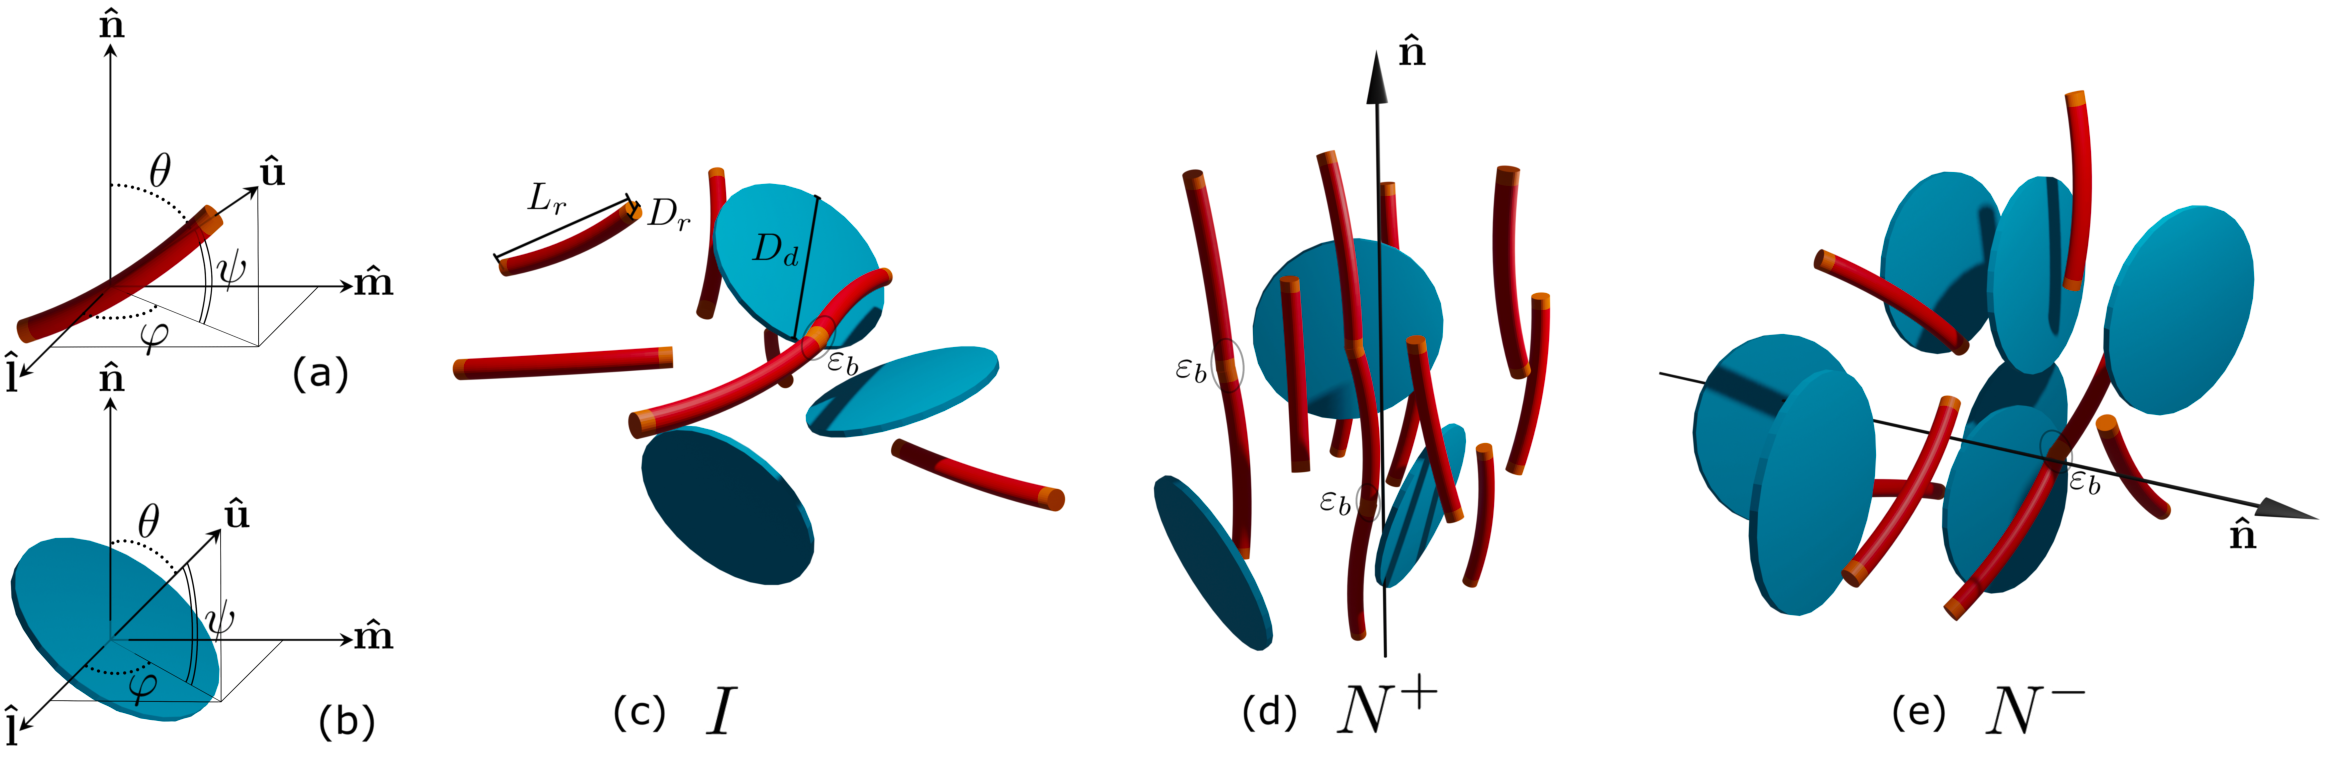
\includegraphics[width=\textwidth]{figures/chapter-3/FIG1}
  \caption{Schematic representation of the various liquid crystal phases emerging for discs mixed with polymerizing rods: (a) - and (b) - Principal angles describing the orientation $\bhu$ of a single rod monomer - and disc - with respect to the molecular director $\bn$  with $\theta$ denoting the polar angle, $\varphi$ the azimuthal angle and $\psi = \frac{\pi}{2} - \theta $ the meridional angle.  (c) Isotropic phase. (d) polymer uniaxial nematic phase $N^+$. (e) discotic uniaxial nematic phase $N^-$ in which the reversibly polymerizing rods are dispersed {\em anti-nematically}.}
  \label{fig:cartoon}
\end{figure*}

An intriguing question in relation to the above is the following:  Can the hierarchical organization of reversible polymers be controlled by the addition of non-adsorbing shape-dissimilar components that affect the way they align? Indeed, for chromonics it is known that the presence of additives can bring about condensation or reorientation of the reversible stacks, thereby changing their phase behavior through subtle modifications of the system entropy \cite{tortora2010}.  Recent experiments on  clay nanosheets mixed with reversibly polymerizing tubuline rods have demonstrated that these mixtures remain stable against flocculation and provide a testbed for exploring entropy-driven phase behavior of biopolymer-platelet mixtures \cite{kato2018}.
Furthermore, it is well established that mixing prolate (rod-shaped) colloids with their  oblate  counterparts  generates a strong coupling between the  orientations of both components leading to organizations with mixed nematic and anti-nematic symmetries. Numerous theoretical studies starting with the early work of Alben \cite{alben1973} have attempted to rationalize the intricate isotropic-nematic  phase behavior of these mixtures  placing particular emphasis on stabilizing the highly sought-after biaxial nematic phase in which both components are aligned along mutually perpendicular directions thus generating a fluid with an orthorhombic ($D_{2h}$) symmetry  \cite{stroobants1984,campallenbolhuisfrenkel,sokolova1997,vanakaras1998,vanakaras2001, matsuda2003,jacksonbiaxrev,varga2002,galindo2,wensinkrodplate,wensinkbiaxial}. Similar kinds of  anti-nematic or biaxial symmetries could arise when dispersing rod-shaped colloids in a thermotropic liquid crystal under appropriate anchoring conditions \cite{matsuyama2010,mundoor2018}. Anti-nematic order has been shown to naturally emerge in porous smectic structures of  shape-persistent nanorings \cite{avendano2016,wensinkavendano2016} or may be realized with the help of external electromagnetic fields as was demonstrated for clay nanosheets \cite{dozov2011} and for discs in the presence of associating magnetic beads \cite{perouklapp2020}.  In this study we wish to build upon the preceding concepts and explore hierarchical self-organization of reversible polymers in the presence of disc-shaped particles. An example of colloidal discs that could be envisaged are clay nanosheets that consist of nanometer-thick discotic particles with a very high diameter-to-thickness ratio. These particles find widespread use in industrial soft matter and are at the basis of many colloidal-polymer composite materials \cite{balazs1998,ginzburg2000}. The clay sheets on their own, provided they do no gelate in crowded conditions,  have a natural tendency to align and form various types of liquid crystals, including nematic phases \cite{kooij1998,gabriel2005,michot2006,paineau_jpcb2009}. When mixed with  reversibly polymerizing components in the absence of strong disc-polymer attractions,  the discs not only induce orientational "templating" of the supramolecular polymers \cite{asdonk2017}, they also influence the mixing entropy of the system which must have  consequences for polymer growth and  phase behavior \cite{taylorherzfeld1991,vdschoot1994epl}. It is precisely these combined entropic effects that we wish to examine more closely in this work. To this end, we formulate a simple model (Section II) that we subsequently cast into  a  particle-based theory (Section III) that features reversible association and accounts for all relevant entropic contributions on the approximate second-virial level. The orientation degrees of freedom of the species are treated using a number of simplified variational approaches that render our theory algebraically manageable.    We stress that our primary attention in this work goes to mixed-shape nematic phases and we do not consider partially crystallized states that may become stable at elevated packing conditions where our theoretical approach is no longer applicable.


Our study broadly falls into two parts. In the first part (Section IV) we explore the molecular weight  distribution in mixtures in which the polymers are organized either nematically or {\em anti-nematically}. The latter state can be realized at elevated disc concentrations where  correlations between the discs are strong enough to generate nematic order of the discotic subsystem which in turn, enforces the supramolecular rods to align perpendicular to the discotic director in such a way that the overall system retains its  uniaxial $D_{\infty  h}$ point group symmetry (\fig{fig:cartoon}(e)). Whereas reversible polymers in a conventional nematic organization are distributed along a near-exponential form with minor non-exponential corrections at short lengths \cite{kuriabova2010},  we argue that {\em anti-nematic} living polymers may, under certain conditions, exhibit a strong non-exponential weight distribution with the most-probable polymer size being oligomeric rather than monomeric. 

In the second part of the manuscript (Section V and VI) we explore the isotropic-nematic phase behavior of the mixed systems by focusing on the uniaxial nematic phases, which seems to be the prevailing nematic symmetry for strongly shape-dissimilar mixtures \cite{wensinkrodplate,campallenbolhuisfrenkel,varga2002,matsuda2003,jacksonbiax}. Our theoretical model is generic and should be applicable to a wide range of different monomer-disc size ratios and temperatures. We discuss the key features for a few exemplary mixtures. One of them is a distinct azeotrope that develops for the isotropic-polymer nematic coexistence, suggesting a strong orientational templating effect imparted by volume-excluded interactions between the polymers and the discs.  Furthermore,  under certain disc-monomer size constraints,  a remarkable four-phase equilibria appears involving a simultaneous coexistence of isotropic gas and liquid phases along with two fractionated uniaxial nematic phases. In Section VII we discuss our findings in relation to recent colloid-polymer models where similar multiphase equilibria have been reported. We end this work with formulating the main conclusions along with some perspectives for further research in Section VIII. 


\section{Model}


In this study, we focus on mixtures of tip-associating rod-shaped monomers with limited backbone flexibility  mixed with rigid discs. An overview of the basic particle shapes is given in \fig{fig:cartoon}. We assume that each rod monomer is equipped with identical attractive patches at either tip such that each rod end can only form a single bond  with an adjacent rod tip producing a linear polymer. The rods do not associate into multi-armed or ring-shaped polymers. We further assume that all species retain their basic fluid order such that the respective density distributions remain uniform in positional space (but not necessarily in orientational phase space). We do not account for the possibility of hexagonal columnar phases formed by (pure) polymers at high monomer concentration and low temperature combined with elevated polymer backbone flexibility  \cite{taylorherzfeld1991,schoot1996}. In fact, discs too may form columnar structures at packing fraction exceeding typically 40 \% \cite{frenkelcol1989,veerman1992,kooij_nature2000} which goes beyond the concentration range we consider relevant here.  Interactions between the polymer segments and the discs are assumed to be purely hard with the only energy scale featuring in the model being the non-covalent bond energy $\varepsilon_{b}$ between the monomers.

 Contrary to previous modelling studies of rod-discs mixture we focus here solely on uniaxial nematic phases and ignore the possibility of biaxial order in which both components align along mutually perpendicular directors. Our focus is motivated by the strong expectation that excluded-volume interactions between the polymers and the discs, which are the principal entropic forces behind generating nematic order \cite{Onsager}, are too disparate to guarantee such orthorhombic nematic symmetry to be stable. Previous theoretical studies \cite{jacksonbiaxrev,varga2002,jacksonbiax,wensinkrodplate,wensinkbiaxial} as well as experiments \cite{kooijlangmuir2000,kooijprl2000,woolston2015} and simulations \cite{campallenbolhuisfrenkel,galindo1,galindo2} on mixed-shape colloids  suggest that strongly unequal excluded volumes indeed favour demixing into strongly fractionated uniaxial nematic phases.  In view of the basic symmetry difference  between the linear polymer and disc, we  then anticipate a rod-based uniaxial phase (denoted $N^{+}$,  \fig{fig:cartoon}(d)) in which the discs are distributed  anti-nematically throughout the uniaxial matrix. Conversely, when the discs outnumber the polymers,  a disc-based uniaxial nematic ($N^{-}$,   \fig{fig:cartoon}(e)) is formed in which the aggregating rods adopt anti-nematic order. The onset of biaxial order emerging from these uniaxial reference phases can be estimated from a simple bifurcation analysis discussed in Appendix B. 
 
 
\subsection{Second-virial Theory for Reversible Polymers mixed with rigid discs}


We start with formulating the free energy per unit volume $V$ of a mixture of discs with density $\rho_{d}(\oma) $ and reversibly polymerizing rods. We define $\rho_{r}(\ell, \oma)$ as the number density of monomer segments  aggregated into a polymeric rod with contour length $\ell L$  and orientation described by unit vector $\oma$.  The aggregation number or polymerization degree is specified by the index $\ell =1,2,3,...$.  Let us write the free energy per unit volume of the mixture as follows \cite{kuriabova2010,wensink_mm2019}:
 \begin{align}
& \frac{  F}{ V}  \sim  \sum_{\ell} \int  d \oma   \left [ \ln \left (4 \pi \Lambda_{r} \rho_{r} (\ell, \oma) \ell^{-1}  \right ) - 1 \right ] \ell^{-1} \rho_{r} (\ell, \oma) \nonumber \\ 
& +     \int  d \oma   \left [ \ln \left ( 4 \pi \Lambda_{d} \rho_{d} ( \oma)   \right ) - 1 \right ]  \rho_{d} (\oma)  + \frac{F_{as}}{V} +  \frac{F_{wlc}}{V} + \frac{F_{ex}}{V} \nonumber \\ 
 \label{free}
\end{align}
Without loss of generality,  all energies are implicitly expressed in units of thermal energy $k_{B}T$ (with $k_{B}$ Boltzmann's constant and $T$ temperature). Furthermore, $\Lambda_{r/d}$ are the thermal volumes of the species  which are immaterial for the thermodynamic properties we are about to explore. The factor $4 \pi$ is included for convenience and equals the unit sphere surface representing the orientational phase space. 
The total rod monomer concentration $\rho_{r0}$ is a conserved quantity so that $\rho_{r0} = \sum_{\ell} \int  d \oma \rho_{r}(\ell, \oma )$. Likewise, $\rho_{d0} = \int d \oma \rho_{d} (\oma)$ represents the number  density of discs.
The first two terms are related to the ideal gas or mixing entropy and describe the ideal translation and orientational entropy of each polymer  and disc, respectively.
The third contribution in \eq{free} represents an association energy that drives end-to-end aggregation of the  monomer segments. It reads: 
 \beq
\frac{F_{as}}{V}  =  \varepsilon_{b}  \sum_{\ell} \int d \oma \ell^{-1} \rho_{r}(\ell, \oma) (\ell -1 ) 
 \label{fas} 
 \eeq
 The free energy per unit volume arising from the polymerized rod segments follows  from the bond potential $\varepsilon_{b}$ between two adjacent rod segments and the number density  $\rho_{a}(\ell, \oma) = (1/\ell) \rho_{r}(\ell, \oma)$ of polymers with aggregation number $\ell  $  each containing  $\ell -1$ bonds. Being normalized to the thermal energy the potential $\varepsilon_{b}$ serves as an {\em effective} temperature scale. At strongly reduced temperature ($\varepsilon_{b} \ll 0$) the association energy is minimised when all monomers  join together into a single long  polymer, while at high temperature ($\varepsilon_{b} \gg 0$) polymerization is strongly suppressed. If $-\varepsilon_{b}$ is of the order of the thermal energy $k_{B}T$, the single chain configuration is highly unfavorable in view of the mixing entropy that favors a broad distribution of aggregates with strongly disperse contour lengths. This we will explore more systematically in Section IV.  

\subsection{Backbone flexibility}

The second last term in \eq{free} represents the effect of polymer flexibility through a correction to the  original orientational entropy (first term in \eq{free}) that accounts for the internal configurations of a so-called worm-like chain \cite{Vroege92}. This leads to a  strongly non-linear term with respect to the segment density \cite{khokhlov82,kuriabova2010}: 
\beq
  \frac{F_{wlc}}{V} = - \frac{2L_{r}}{3\ell_{p}} \sum_{\ell} \int d \oma [ \rho_{r}(\ell, \oma)]^{1/2} \nabla^{2}  [ \rho_{r}(\ell, \oma)]^{1/2}
  \label{wlc}
\eeq
where $\nabla^{2} $ denotes the Laplace operator on the unit sphere. 
The persistence length $\ell_{p}$ measures the  typical length scale over which local orientational fluctuations of the segments are correlated.  In our model we assume that the rod segments are only slightly flexible \cite{khokhlov82}  so that $\ell_{p} \gg \ell$ suggesting that the main orientational entropy stems from the rigid body contribution that is subsumed into the ideal gas term in \eq{free}. The worm-like chain correction   
vanishes in the somewhat unnatural situation where all polymers, irrespective of their contour length, are perfectly rigid and the persistence length tends to infinity ($\ell_p \rightarrow \infty$).  


\subsection{Excluded-volume entropy}

The last contribution in \eq{free} is the excess free energy that incorporates all excluded-volume driven interactions between the stiff polymers and discs. Assuming all interactions to be strictly hard, we write following Ref. \cite{stroobants1984}:
\begin{align}
& \frac{F_{ex}}{ V}  =  \frac{1}{2}   \sum_{\ell, \ell^{\prime}}  \iint d  \oma  d \oma^{\prime} \rho_{r}(\ell, \oma)  \rho_{r}(\ell^{\prime}, \oma^{\prime})  2  L_{r}^{2} D_{r}  | \sin \gamma |  \nonumber \\
& +    \sum_{\ell}  \iint d  \oma  d \oma^{\prime} \rho_{r}(\ell, \oma) \rho_{d}( \oma^{\prime})  \frac{\pi}{4}  L_{r} D_{d}^{2}  | \cos \gamma |  \nonumber \\
& +  \frac{1}{2} \iint d  \oma  d \oma^{\prime} \rho_{d}( \oma) \rho_{d}( \oma^{\prime})  \frac{\pi}{2} D_{d}^{3}  | \sin \gamma |  
\label{fex}
\end{align}
where $L_{r,d}$ and $D_{r,d}$ denote the length and diameter of the cylindrical building blocks (see \fig{fig:cartoon}(b)).  We assume all polymers and discs to be sufficiently slender, i.e., $L_{r}/D_{r} \gg 1$ and $D_{d}/L_{d} \gg 1$ so that finite-thickness corrections to the excluded volume terms above can be neglected.   Next we formally minimize the free energy with respect to the polymer segment distribution
\beq
\frac{\delta}{\delta \rho_{r} ( \ell , \oma )} \left ( \frac{ F}{V} - \lambda_{r} \sum_{  \ell} \int d \oma \rho_{r}( \ell, \oma ) \right ) =0
\label{el1}
\eeq
and to the one-body density of the discs
\beq
\frac{\delta}{\delta \rho_{d} ( \oma )} \left ( \frac{ F}{V} - \lambda_{d}  \int d \oma \rho_{d}(  \oma ) \right ) =0
\label{el2}
\eeq
The Lagrange multipliers $\lambda_{r,d}$ ensure that the total concentration of each species (monomers and discs) be preserved.  The coupled Euler-Lagrange (EL) equations can be rendered tractable by expanding the orientation-dependent kernels that depend on the enclosed angle $\gamma$ between the main particle orientation axes, as we will show next.


\subsection{Molecular weight-distribution from second-polynomial approximation}

A commonly employed method to cast the free energy in a more tractable form is to express the trigonometric functions featuring in the excluded-volume \eq{fex} in terms of a bilinear expansion in Legendre polynomials \cite{lakatos,kayser,lekkerkerker84}. Truncating this expansion after the second-order contribution leads to a simplified theory that has been explored previously for rod-plate mixtures \cite{stroobants1984,jacksonbiax} as well as in the context of  rods with fixed length polydispersity \cite{sollichonsagerP2}. For the present mixture, the approximation should be adequate if the nematic order of either component is not too strong. We  write:
\begin{align}
| \sin \gamma | &= \frac{\pi}{4} - \frac{5 \pi }{32} \pp(\cos \theta) \pp(\cos \theta^{\prime}) + \cdots \nonumber \\
| \cos \gamma | &= \frac{1}{2} + \frac{5 }{8} \pp(\cos \theta) \pp(\cos \theta^{\prime}) + \cdots
\label{p2expansion}
 \end{align}
in terms of the second Legendre polynomials $\pp(x) = \frac{3}{2} x^{2} - \frac{1}{2}$. The  orientation of each particle is described by a polar angle $\theta$ and azimuthal angle $\varphi$ defined with respect to the nematic director $\bn$ (see \fig{fig:cartoon}a and b). Let us define a set of  {\em size-specific} nematic order parameters for the polymer:
\begin{align}
S_{r \ell} = \rho_{r \ell}^{-1} \int d \oma \rho_{r}(\ell, \oma) \pp (\oma \cdot \bn) 
\label{sr} 
\end{align}
with $\rho_{r \ell } = \int d \oma \rho_{r} (\ell, \oma)$ a partial number density of rod segments belonging to polymers of length $\ell L$. Likewise we find for the discs:
\begin{align}
S_{d} = \rho_{d0}^{-1} \int d \oma \rho_{d}( \oma) \pp (\oma \cdot \bn) 
\end{align}
These order parameters allow us to distinguish between an isotropic fluid ($S_{r \ell}=S_{d}=0$), a polymer-dominated uniaxial nematic fluid ($N^{+}$: $S_{r \ell} > 0$, $S_{d} <0$) and a discotic one ($N^{-}$: $S_{r} < 0$, $S_{d} >0$), as sketched in \fig{fig:cartoon}d and e, respectively.  With the aid of these expansions, the excess free energy can be written in terms of a simple bilinear dependence on the nematic order parameter:
\begin{align}
 \frac{F_{ex}}{ V}   \sim & \rho_{r0}^{2}   \left ( 1 - \frac{5}{8}  \bar{S}_{r }^{2} \right ) +  2 q \rho_{r 0} \rho_{d}   \left ( 1 + \frac{5}{4} \bar{S}_{r} S_{d}   \right ) \nonumber \\
& + z \rho_{d}^{2}  \left ( 1 - \frac{5}{8} S_{d}^{2}  \right ) 
\label{fexsim}
 \end{align}
 Here, we have implicitly renormalized the free energy and species densities in terms of the isotropic excluded volume of the monomeric rods  $v_{rr} = \frac{\pi}{4} L_{r}^{2} D_{r}$. The excess free energy thus only depends on the excluded-volume {\em ratios}    $q= v_{rd}/v_{rr}$ and $z =v_{dd}/v_{rr}$  with $v_{rd} = \frac{\pi}{16} L_{r} D_{d}^{2} $ and $v_{dd} = \frac{\pi^{2}}{16} D_{d}^{3}$ denoting the isotropized  monomer-disc and disc-disc excluded volumes, respectively.
Furthermore, the bar denotes a molecular-weight average of the nematic order parameter associated with the polymers:
\begin{align}
\bar{S}_{r} &= \rho_{r0}^{-1}  \sum_{\ell} \rho_{r\ell} S_{r \ell} 
\label{srav}
\end{align}
Similarly, the coupled EL equations may be cast as follows: 
\begin{align}
& \ell^{-1} \ln [ 4 \pi \rho_{r} (\ell, \oma ) \ell^{-1} ]   = \lambda_{r}  + \varepsilon_{b} \ell^{-1} +  a_{r} \pp(\oma \cdot \bn) \nonumber \\ 
&  +\frac{L_{r}}{3\ell_{p}} \frac{\nabla^{2} [ \rho_{r} (\ell , \oma)]^{1/2}}{ [ \rho_{r} (\ell , \oma)]^{1/2} }
\label{lnrhor}
\end{align}
and
\begin{align}
\ln [ 4 \pi  \rho_{d} (\oma )] & = \lambda_{d}  + a_{d} \pp(\oma \cdot \bn)  
\label{lnd}
\end{align}
The uniaxial order parameters that feature in the EL equations are specified as follows:
\begin{align}
a_{r} &=    \frac{5 }{4}  ( \rho_{r0}  \bar{S}_{r} -   2  q\rho_{d0}  S_{d} )  \nonumber \\
a_{d} &=   \frac{5}{4} (  z \rho_{d0}   S_{d}  -  2q  \rho_{r0} \bar{S}_{r} )  
\label{alphabeta}
\end{align}
We  are now equipped to explore the equilibrium polymer length distribution  $\rho_{r \ell} =  \int d \oma \rho_{r} (\ell, \oma)$ corresponding to the basic fluid symmetries we consider (cf. \fig{fig:cartoon}).

\section{Polymer length distributions}

\subsection{Isotropic fluid}

In the isotropic phase, all nematic order parameters are strictly zero. Applying conservation of monomers to \eq{lnrhor} and performing some algebraic rearrangements we find a geometric distribution (i.e., the discrete analog of the exponential distribution):
\begin{align}
\rho_{r \ell } & =   \ell e^{ \varepsilon_{b} + \lambda_{r} \ell }  \nonumber \\
&= \ell e^{ \varepsilon_{b}} \left ( 1 - m_{I}^{-1} \right ) ^{\ell} \label{disi}
\end{align}
in terms of the mean aggregation number:
\beq
m_{I} =  \frac{\sum_{\ell} \rho_{a}(\ell) \ell  }{\sum_{\ell} \rho_{a}(\ell) } = \frac{1}{2} \left ( 1+ \sqrt{1+ 4 \rho_{r0} e^{-\varepsilon_{b}} }\right ) 
\label{miso}
\eeq
which, as expected, goes up monotonically with increasing monomer concentration  $\rho_{r0} $ and also increases when the effective temperatures  $\varepsilon_{b}$ grows more negative.  Since there is no global particle alignment whatsoever, the presence of the discs does not influence the polymerization process, and the polymer molecular-weight distribution is independent from the disc concentration.  

\subsection{Uniaxial nematic fluid}

The decoupling of polymeric rods and discs  is no longer  valid  for a nematic fluid where the alignment direction of one component is strongly affected by the amount of orientational ``templating" it experiences from the other component.
The polymer density  follows  from  \eq{lnrhor} and can be written in an exponential form:
\begin{align}
4 \pi \rho_{r} (\ell , \oma) &= \ell \exp [\varepsilon_{b} + \ell \lambda_{r} +  \tilde{a}_{r} \ell \pp(t) ] 
\label{rhorfull}
\end{align}
with $t = \cos \theta $. The three basic contributions affecting the polymer molecular weight  distribution  in a (uniaxial) nematic fluid are easily identified in the argument; the first denotes  monomer-monomer bonding while the second term  enforces monomeric mass conservation. The third one is the most interesting one; it encapsulates the templating effect associated with nematization of the discs as per \eq{alphabeta}. Here,  we have introduced $a_{r}$ as a renormalized version of the one in \eq{alphabeta}:
\beq
\tilde{a}_{r} =  a_{r} + \xi 
\eeq
The factor $\xi$ depends on both $a_{r}$ itself and on the polymer persistence length $\ell_{p}$. It accounts for the finite polymer flexibility and vanishes for strictly rigid polymers ($\ell_{p} \rightarrow \infty$). The corresponding expressions are given in the Appendix. As noted previously, the multiplier $\lambda_{r}$ featuring in \eq{rhorfull}  follows from monomer mass conservation:
\beq
  \sum_{\ell=1}^{\infty}  \int d \oma \rho_{r}(\ell, \oma)  = \rho_{r0}
 \label{como}
\eeq
The summation can be resolved analytically and we find:
\beq
\rho_{r0} = e^{\varepsilon_{b}} \frac{1}{2} \int_{-1}^{1} dt \frac{ e^{W(t) }}{ ( e^{W(t)} -1)^{2}}
\eeq
The molecular-weight averaged  nematic order parameter \eq{srav} is then given by:
\beq
\bar{S}_{r} = \rho_{r0}^{-1} e^{\varepsilon_{b}} \frac{1}{2} \int_{-1}^{1} dt  \frac{ \pp(t) e^{ W(t) }}{ (  e^{ W(t)} -1)^{2}}
\eeq
The two conditions above are intricately coupled given that $\tilde{a}_{r}$ depends on both $\bar{S}_{r}$  and $S_{d}$ via \eq{alphabeta}. Convergence of the summation \eq{como}  requires that the argument be negative:
 \beq
 W(t) = \lambda_{r} + \tilde{a}_{r} \pp(t) < 0, \hspace{0.3cm} \textrm{all} \hspace{0.1cm}  t
 \eeq
 Noticing that $ -1/2 \leq|| \pp || \leq 1$ one then finds that $\lambda_{r}$ should satisfy:
 \begin{align}
- \lambda_{r} & <  |\tilde{a}_{r} | \hspace{0.3cm} (N^{+}) \nonumber \\
- \lambda_{r} & <  |\tilde{a}_{r}/2 |\hspace{0.3cm}  (N^{-}) 
 \end{align}
and it is tempting to introduce a rescaled  normalization constant $\lambda_{r}^{\prime}$ that is strictly positive ($\lambda_{r}^{\prime} > 0$) for both phases. With this, we recast:
  \begin{align}
W(t) =  
\begin{cases}
\frac{3}{2} \tilde{a}_{r} (t^{2} -1) - \lambda_{r}^{\prime} \hspace{0.5cm}  (N^{+})   \\
\frac{3}{2} \tilde{a}_{r} t^{2}  - \lambda_{r}^{\prime} \hspace{1.2cm}  (N^{-}) 
\end{cases}
 \end{align}
 Unlike for the isotropic phase, the normalization constant $\lambda_{r}^{\prime}$ can not be resolved in closed form. The  molecular-weight distribution of the polymer follows from integrating \eq{rhorfull} over all orientations $\oma$:
 \beq
 \rho_{r \ell} = \ell e^{\varepsilon_{b}} \frac{1}{2} \int_{-1}^{1} dt e^{\ell W(t)}
 \eeq
The uniaxial nematic order parameter $S_{r \ell}$ associated with a  polymer of length $\ell$ is easily found from:
\beq
S_{r \ell} = -\frac{1}{2} \left \{ 1 + \frac{1}{\tilde{a}_{r} \ell}  - \frac{1}{      F  \left (  \sqrt{3 \tilde{a}_{r} \ell/2}   \right ) \sqrt{    \tilde{a}_{r} \ell /3 }  }  \right \}  
\label{spol}
\eeq
in terms of Dawson's integral $F(x) = e^{-x^{2}} \int_{0}^{x}e^{y^{2}}dy$ \cite{abram}. The discotic nematic order parameter $S_{d}$  easily follows from the above expression upon substituting $\tilde{a}_{r} \ell \rightarrow a_{d}$.   A little reflection of \eq{spol} tells us the following; since $a_{r}$ does not depend explicitly on the aggregation number $\ell$, the nematic order parameter $S_{r \ell}$ must be a monotonically increasing function of the polymerization degree $\ell $; the longer the polymers the stronger their nematic ($ a_{r} >0$) or anti-nematic ($ a_{r} <0$) alignment in the mixed nematic fluid. This effect becomes systematically weaker for increasingly flexible polymers as can easily be inferred from the above expression by comparing  $S_{r \ell}$ versus $\ell$ for rigid polymers $(\xi =0)$ versus the case of slightly flexible ones ($\xi $ nonzero but small) for any given value for $a_{r}$. 

% TODO: reshape to fit in single column text
\begin{figure}
  \includegraphics[width=\linewidth]{figures/chapter-3/FIG2}
  \caption{Polymer molecular-weight distributions $\rho_{r \ell}$ and corresponding  uniaxial nematic order parameter $S_{r \ell}$ as a function of the polymer length $\ell$ for (a) a typical polymer nematic $N^{+}$ and (b) discotic nematic phase $N^{-}$. The effective temperature $\varepsilon_{b}$ is color-coded.   
  (c) Most Probable Length (MPL) in terms of the effective temperature $\varepsilon_{b}$. Fixed parameters: persistence length $\ell_{p} = 3$, disc mole fraction $x = 0.5$, overall concentration $\rho = 3$, excluded-volume {\em ratios} $q = \frac{1}{4}\frac{L_{r}}{D_{r}}$ and $z=\pi q$ with monomer aspect ratio $L_{r}/D_{r} =10$.  }
  \label{fig:distributions}
\end{figure}
 
Let us now examine a concrete example by picking a dense uniaxial discotic nematic  doped with polymerizing rods. The polymers are dispersed anti-nematically within the discotic fluid as indicated in \fig{fig:cartoon}(e).   In specifying the shape of the rods and discs, we can distinguish between  so-called {\em symmetric} mixtures \cite{stroobants1984}, in which the excluded-volume  between two monomers, a monomer and a disc and two discs are all equal, so that $q = 1$ and $z = 1$ and {\em asymmetric mixtures} composed of species with  strongly disparate excluded volumes.   Our principal attention goes to the latter systems which arise more naturally in an experimental context when mixing, for instance, tip-associating colloidal rods such as {\em fd} \cite{fraden-tmv-baus,dogic-fraden_fil} with clay platelets \cite{davidson-overview}. The molecular-weight distributions of some mixtures of this nature are shown in \fig{fig:distributions}.

 \fig{fig:distributions}(a) relates to the uniaxial polymer-dominated nematic phase ($N^+$) and demonstrates an exponential probability distribution  whose shape can be tuned by changing the effective temperature of the system. As expected, the tail of the distribution grows upon decreasing the temperature, which would give longer polymers. A more interesting scenario shows up for the discotic nematic phase ($N^-$) in \fig{fig:distributions}(b), where the distributions are no longer monotonically decreasing. The maximum of the distributions corresponds to the most probable length of the polymers for each system, which depends quite sensitively on the effective temperature as we  observe in \fig{fig:distributions}(c). Reversible polymerization within an anti-nematically organization  thus leads to a strong manifestation of oligomeric polymers at the expense of its monomeric counterparts. We  note that the orientational order associated with the anti-nematic oligomers remains relatively mild (particularly at larger temperature $\varepsilon_{b}$) so that the second-polynomial truncation should not be too severe.


As we will see during the incoming sections of this manuscript, the overall particle concentration and disc molar fraction  associated with \fig{fig:distributions} may correspond to  regions of the phase diagram where the uniform nematic system is in fact thermodynamically unstable with respect to some kind of phase separation. The molecular-weight distributions should therefore be interpreted under the caveat that monophasic nematic fluidity is preserved and that any demixing process is somehow suppressed. We wish to add that the non-monotonic features of the anti-nematic polymer molecular-weight distribution are also present at conditions where monophasic anti-nematic order is found to be stable.  Next we address the  thermodynamic stability of the mixtures  within the context of a Gaussian variational theory. 

\section{Isotropic-nematic phase behavior}

At conditions where (anti-)nematic order is strong, the previously used polynomial-based expansion truncated after ${\mathcal P}_{2}$ [\eq{p2expansion}] is no longer appropriate and  a cumbersome inclusion of multiple higher-order terms becomes necessary \cite{lekkerkerker84,wensinkbiaxial}. A more technically expedient route towards exploring the thermodynamics of strongly ordered nematic fluids is to use a simple Gaussian parameterization of the orientational probability \cite{odijkoverview,Vroege92}.  Following \cite{wensink_mm2019} we express the polymer molecular-weight distribution in a factorized form:
\beq
\rho_{r} (\ell , \oma ) = \rho_{r \ell} f_{G} (\oma) 
\label{pfac}
\eeq
where $f_{G}$ is a normalized Gaussian distribution with a variational parameter that is proportional to either the degree  nematic  order ($\alpha^{(1)} > 0$) or anti-nematic order  ($\alpha^{(2)} > 0$).  The corresponding Gaussian distributions for the polar angles corresponding to these different nematic symmetries are given by \cite{wensinkrodplate}:
\beq
f_{G} (\oma) \sim  
\begin{cases}
\frac{\alpha^{(1)}}{4 \pi } \exp (-\frac{1}{2}\alpha^{(1)} \theta^{2} ) , \\
\sqrt{ \frac{ \alpha^{(2)} }{ (2 \pi )^{3} } } \exp (-\frac{1}{2} \alpha^{(2)} \psi^{2} )
\end{cases}
\label{gaussians}
\eeq
where $\psi = \frac{\pi}{2} - \theta$ ($-\pi/2 < \psi < \pi/2$) denotes a meridional angle (see \fig{fig:cartoon}a). The Gaussians operates on the domain $0 < \theta < \pi/2$ and must be complemented by their mirror $f_{G} (\pi - \theta )$ for $\pi/2 < \theta < \pi$  given that all nematic phases are required to be strictly apolar. The Gaussian representations are appropriate only for strong nematic order ($\alpha \gg 1$). They are clearly inadequate for isotropic systems since the probabilities reduce to zero when $\alpha \rightarrow 0$ instead of reaching a constant.  Obviously,  we  apply the same distributions to the discs with $\alpha_{d}^{(1)}$ and $\alpha_{d}^{(2)}$ denoting the variational parameters quantifying the amount of (anti)nematic order of the discs. The disc probability density is then equivalent to \eq{pfac}:
\beq
\rho_{d} (\oma ) = \rho_{d0} f_{G} (\oma) 
\eeq
A major advantage of using  Gaussian trial functions is that we may apply  asymptotic expansion of the various free energy contributions \cite{odijkoverview} which are valid in the limit $\alpha \rightarrow \infty$. In particular, it can be shown that the double orientational averages over the sine and cosine in \eq{fex} up to leading order in $\alpha$ take a simple analytic form \cite{wensinkrodplate}.  In the general case in which particles with equal nematic signature (nematic or anti-nematic) do not necessarily have the same degree of alignment the asymptotic averages read:
\begin{align}
\langle \langle | \sin \gamma | \rangle \rangle_{11} & \sim \sqrt{ \frac{\pi}{2} \left ( \frac{1}{\alpha^{(1)}} + \frac{1}{\alpha^{(1\prime)}} \right ) } \nonumber \\  
    \langle \langle | \cos \gamma | \rangle \rangle_{12} & \sim  \sqrt{ \frac{2}{\pi} \left ( \frac{1}{\alpha^{(1)}} + \frac{1}{\alpha^{(2)}} \right ) } \nonumber \\ 
    \langle \langle | \sin \gamma | \rangle \rangle_{22} & \sim \mathcal{F} (\alpha^{(2)}, \alpha^{(2\prime)})
    \label{sinav}
\end{align}
Here,  the double brackets denote the orientational averages featuring in the excess free energy \eq{fex} with $ \langle \cdot \rangle = \int d \oma f_{G} (\oma) $. The symmetry of nematic order clearly matters since the anti-nematic case features a distinct logarithmic dependence. The function ${\mathcal F}$ reads in explicit form:

\beq
 {\mathcal F}(\alpha^{(2)},\alpha^{(2 \prime)} ) = \frac{4 \alpha^{(2)} Q -2 (1+Q) \textrm{arctanh} \sqrt{Q}  - (1+Q) \ln (1-Q) +(1+Q) \ln ( 4 \alpha^{(2)} Q) } {2 \pi \alpha^{(2)} Q}
\eeq

in terms of the ratio $Q=  \alpha^{(2\prime)}/ \alpha^{(2)}$ with $\alpha^{(2)}$ and $\alpha^{(2\prime)}$ quantifying the anti-nematic order parameters of two polymeric species differing in length. Note that generally, $\alpha^{(2)} \neq \alpha^{(2\prime)}$. The expression becomes a lot more manageable if all polymers are assumed to exhibit an equal degree of alignment, irrespective of their length. Then, $Q=1$ and \cite{wensink2001}:
\beq
{\mathcal F}(\alpha^{(2)})  =  \frac{2}{\pi} \left ( 1 + \frac{\ln \alpha^{(2)}}{2 \alpha^{(2)}} \right )
\eeq
Similar asymptotic expressions may be obtained for the orientational entropy featuring in the ideal free energy \eq{free}. For strong nematic or anti-nematic order we find, respectively \cite{wensinkrodplate}:
\begin{align}
\sigma_{1} = \langle \ln 4 \pi f_{G} (\oma) \rangle_{1} &\sim \ln \alpha^{(1)} -1  \nonumber \\
\sigma_{2} =\langle \ln 4 \pi f_{G} (\oma) \rangle_{2}   &\sim \frac{1}{2} \left ( \ln \alpha^{(2)} + \ln \frac{2}{\pi} -1 \right )  
\label{sigma12}
\end{align}
The worm-like chain entropy \eq{wlc} too can be quantified within in the Gaussian limit which leads to:
\begin{align}
\langle  f_{G}^{1/2} (\oma) \nabla^{2} f_{G}^{1/2} (\oma)  \rangle_{1} & \sim -\frac{\alpha^{(1)}}{2} \nonumber \\ 
\langle  f_{G}^{1/2} (\oma) \nabla^{2}  f_{G}^{1/2} (\oma)  \rangle_{2} & \sim  
-\frac{\alpha^{(2)}}{4} 
\end{align}
We infer that the loss of conformational entropy of an {\em anti-nematic} polymer is half that of a nematic polymer. This suggests that a worm-like chain is able to retain more of its internal configurations when aligned anti-nematically than in a nematic organization of equal strength. With all the orientational averages specified, we  now turn to computing the free energy and its derivatives. 



\subsection{Polymer nematic phase ($N^{+}$)}

We first focus on the case of the polymer-dominated nematic phase which is expected to be stable at elevated monomer concentration and low disc mole fraction.  Inserting the asymptotic orientational averages formulated above into the corresponding entropic contributions in \eq{free} we obtain the following algebraic expression for the free energy density (in units thermal energy $k_{B}T$ per randomized monomer excluded volume $v_{rr}$):
\begin{align}
   & \frac{F^{N^{+}}}{V}  \sim  \sum_{\ell }  \rho_{r \ell} \ell^{-1}  \left [ \ln \rho_{r \ell} \ell^{-1}  -1 - \varepsilon_{b}  + \sigma_{1}(\alpha_{r \ell}) \right ] \nonumber \\
   & + \rho_{d0} \left [ \ln \rho_{d0} -1 + \sigma_{2}(\alpha_{d}) \right ]  \nonumber \\ 
    & + \frac{1}{3\ell_{p}} \sum_{\ell } \rho_{r \ell} \alpha_{r \ell} + \sum_{\ell,\ell^{\prime}} \rho_{r \ell} \rho_{r \ell^{\prime}} h_{r\ell r\ellp} \nonumber \\
    & + 2 q \rho_{d0} \sum_{\ell} \rho_{r \ell} h_{r\ell d} + z \rho_{d0}^{2} \frac{8}{\pi^{2}} \left ( 1+ \frac{\ln \alpha_{d}}{2 \alpha_{d}}   \right ) 
\end{align}
with $h_{ij}$ is short-hand notation for:
\beq
h_{ij} = \sqrt{ \frac{8}{\pi}   \left ( \frac{1}{\alpha_{i}} + \frac{1}{\alpha_{j}} \right )} 
\eeq
where $\alpha_{i}$ and $\alpha_{j}$ should be considered dummy variables for the species-dependent nematic order parameters as specified by the indices $i$ and $j$. 
For later reference we also define:
\beq
g_{ij} = \left (  \frac{8}{\pi} \right)^{1/2}  \left ( 1+ \frac{\alpha_{i} }{\alpha_{j }} \right )^{-1/2}
\eeq
At equilibrium, the species-dependent nematic order parameters $\alpha_{r\ell}$ and $\alpha_{d}$ follow from the minimum conditions:
\begin{align}
    \frac{\partial F/V}{\partial \alpha_{r \ell,d}} &=0 
    \label{dalpha}
\end{align}
The expressions above can be simplified considerably by noting that a small amount  of backbone flexibility causes the nematic alignment to fully decorrelate from the polymer contour length. We then approximate $\alpha_{r \ell} \approx \alpha_{r \ell^{\prime}} = \alpha_{r}$, independent from $\ell$.   Applying \eq{dalpha} we obtain a set of simple algebraic equations:
\begin{align}
      m_{N^{+}}^{-1} \alpha_{r}^{1/2}  &= - \frac{1}{3\ell_{p}} \alpha_{r}^{3/2} + \frac{2}{\sqrt{\pi}}  \rho_{r0} + q \rho_{d0}  g_{rd} \nonumber \\
         \alpha_{d}^{1/2} &=  z \rho_{d0} \frac{8}{\pi^{2}}\left (  \frac{ \ln \alpha_{d} -1}{\alpha_{d}^{1/2}} \right ) 
  + 4 q \rho_{r0} g_{dr} 
  \label{alphaplus}
\end{align}
with $m_{N^{+}}$ the mean aggregation number in the polymer nematic phase.
The  molecular-weight distribution  now becomes strictly exponential, as for the isotropic phase. We write:
\begin{align}
\rho_{r \ell } & = \ell e^{ \tilde{\varepsilon}_{b}} \left ( 1 - m_{N^{+}}^{-1} \right ) ^{\ell} \label{disn}
\end{align}
with an {\em effective} potential $\tilde{\varepsilon}_{b}$ that depends on the orientational entropy:
\beq
\tilde{\varepsilon}_{b} = \varepsilon_{b} - \sigma_{1}(\alpha_{r}) 
\label{tempnplus}
\eeq
Given that $\sigma_{1} >0$, the effective temperature is {\em lower} than the bare one, so that polymerization in the nematic phase is stronger than in the isotropic fluid, as is well established \cite{vdschoot1994epl,vdschoot1994la}. The mean aggregation number in the nematic phase  has an analogous form to \eq{miso}):
\beq
m_{N^{+}}  = \frac{1}{2} \left ( 1+ \sqrt{1+ 4 \rho_{r0} e^{-\tilde{\varepsilon}_{b}} }\right ) 
\eeq
The chemical potentials are obtained from the standard thermodynamic relations $\mu_{r,d}  = \partial (F/V) /\partial \rho_{r0,d0}$. The contribution from the polymers reads:
\begin{align}
\mu_{r}^{N^{+}}  \sim & \ln ( 1 - m_{N^{+}}^{-1}) + \frac{1}{3 \ell_{p}}  +  m_{N^{+}}^{-1} \sigma_{1}(\alpha_{r})  \nonumber \\
& + 2  \rho_{r0}   \frac{4}{\sqrt{\pi \alpha_{r}}}  +   2 q \rho_{d0} h_{rd}
+ \varepsilon_{b} 
\end{align}
while for the discs we find:
\begin{align}
\mu_{d}^{N^{+}}  \sim  & \ln \rho_{d0}  + \sigma_{2}(\alpha_{d})  +   2 q \rho_{r0}  
h_{rd} + 2 z \rho_{d0} 
\frac{8}{\pi^{2}} \left ( 1+ \frac{\ln \alpha_{d}}{2 \alpha_{d}} \right )
\end{align}
The osmotic pressure follows from  the thermodynamic relation $-P = (F - N \mu)/V$ leading to:
\begin{align}
P^{N^{+}} \sim & e^{\tilde{\varepsilon}_{b}} (m_{N^{+}} -1) 
+ \rho_{d0}  +  \rho_{r0}^{2}  \frac{4}{\sqrt{\pi \alpha_{r}}}
 \nonumber \\ 
& +   2 q \rho_{r0}  \rho_{d0} h_{rd}
 + z \rho_{d0}^{2} 
  \frac{8}{\pi^{2}} \left ( 1+ \frac{\ln \alpha_{d}}{2 \alpha_{d}}   \right )
\label{pressurenp}
\end{align}
Note that all pressures are implicitly renormalized in units of the thermal energy $k_{B}T$ per monomer excluded volume  $v_{rr}$.


\subsection{Discotic nematic phase ($N^{-}$)}

Repeating the previous steps for the discotic nematic through simple bookkeeping we write for the free energy of the discotic phase:
\begin{align}
   & \frac{F^{N^{-}}}{V}  \sim  \sum_{\ell }  \rho_{r \ell} \ell^{-1}  \left [ \ln \rho_{r \ell} \ell^{-1}  -1 - \varepsilon_{b}  +\sigma_{2} (\alpha_{r \ell})  \right ] \nonumber \\
   & + \rho_{d0} [ \ln \rho_{d0} -1 + \sigma_{1}(\alpha_{d})  ] + \frac{1}{6\ell_{p}} \sum_{\ell } \rho_{r \ell} \alpha_{r \ell} \nonumber \\ 
   & + \sum_{\ell,\ell^{\prime}} \rho_{r \ell} \rho_{r \ell^{\prime}} 
    \frac{4}{\pi} {\mathcal F} (\alpha_{r \ell}, \alpha_{r \ell^{\prime}}) \nonumber \\
    & + 2 q \rho_{d0} \sum_{\ell} \rho_{r \ell}  h_{r\ell d} + z \rho_{d0}^{2} \frac{4} {\sqrt{ \pi \alpha_{d}}}
\end{align}
The corresponding minimum conditions for the variational parameters under the assumption that all polymer species experience the same degree of orientational order ($\alpha_{r \ell} = \alpha_{r \ell \prime} = \alpha_{r}$) are as follows: 
\begin{align}
     \frac{1}{2} m_{N^{-}}^{-1}  \alpha_{r }^{1/2} &=  - \frac{1}{6\ell_{p}} \alpha_{r }^{3/2} +  \rho_{r0}  \frac{8}{\pi^{2}} 
    \left ( \frac{\ln  \alpha_{r} - 1}{\alpha_{r}^{1/2}} \right )   + q \rho_{d0}  g_{rd} \nonumber \\
 \alpha_{d}^{1/2} &=  z \rho_{d0} \frac{2}{\pi^{1/2}}  + 2 q \rho_{r0} g_{dr}
 \label{alphamin}
\end{align}
The molecular-weight distribution is  analogous to \eq{disn} but with the effective temperature now reading:
\beq
\tilde{\varepsilon}_{b} = \varepsilon_{b} - \sigma_{2}(\alpha_{r}) 
\label{tempnmin}
\eeq
which, as for the case of the polymer nematic phase suggests that particle alignment facilitates polymer growth, although less so for anti-nematic polymers since generally $\sigma_{2}  < \sigma_{1}$ (\eq{sigma12}).  The chemical potential of the polymers and the discs are given by, respectively:
\begin{align}
 \mu_{r}^{N^{-}}   \sim  
& \ln ( 1 - m_{N^{-}}^{-1}) + \frac{1}{6 \ell_{p}}  +  m_{N^{-}}^{-1} \sigma_{2}(\alpha_{r})  \nonumber \\
& + 2  \rho_{r0} 
\frac{8}{\pi^{2}} \left ( 1+ \frac{\ln \alpha_{r}}{2 \alpha_{r}} \right )
+   2 q \rho_{d0}  h_{rd}
+ \varepsilon_{b} \nonumber \\
 \mu_{d}^{N^{-}}  \sim  & \ln \rho_{d0}  + \sigma_{1}(\alpha_{d})  +   2 q \rho_{r0}  
h_{rd} + 2 z \rho_{d0}  \frac{4} {\sqrt{ \pi \alpha_{d}}}
\end{align}
Finally, the pressure of the $N^{-}$ phase reads:
\begin{align}
P^{N^{-}} \sim & e^{\tilde{\varepsilon}_{b}} (m_{N^{-}} -1) + \rho_{d0} +  \rho_{r0}^{2}  \frac{8}{\pi^{2}} \left ( 1+ \frac{\ln \alpha_{r}}{2 \alpha_{r}}   \right )
 \nonumber \\ 
& +   2 q \rho_{r0}  \rho_{d0}  h_{rd}
 + z \rho_{d0}^{2}  \frac{4}{\sqrt{\pi \alpha_{d}}}
\label{pressurenm} 
\end{align}
The thermodynamics of the isotropic phase is easily established from the original free energy \eq{free} because the randomized excluded volumes becomes simple constants, namely  $\langle \langle | \sin \gamma | \rangle \rangle = \pi/4$ and $\langle \langle  | \cos \gamma | \rangle \rangle  = 1/2$. We thus obtain the following expressions for the chemical potentials in the isotropic fluid \cite{wensink_mm2019}:
\begin{align}
  \mu_{r}^{\textrm I} & \sim  \ln ( 1- m_{I}^{-1} )  + 2  \rho_{r0}  +   2 q \rho_{d0}  + \varepsilon_{b} \nonumber \\
   \mu_{d}^{\textrm I} & \sim \ln \rho_{d0}  +   2 z \rho_{d0} + 2 q \rho_{r0} 
  \end{align}
The osmotic pressure  combines the ideal gas and excluded volume contributions and reads:
\begin{align}
   P^{\textrm I}  &\sim  e^{\varepsilon_{b}} (m_{I} -1) + \rho_{d0}  +  \rho_{r0}^{2}
+   2 q \rho_{r0}  \rho_{d0}  + z \rho_{d0}^{2} 
\end{align}
Binodals denoting coexistence between phases of any symmetry may be established from equating chemical potentials and pressures in conjunction with the minimum conditions for the nematic variational parameters, where relevant.  Phase diagrams can be represented in a pressure-composition  ($P-x$) plane or, alternatively, in a density-density representation using $\rho_{r0} = c (1-x)$ and $\rho_{d0}  = cx$ in terms of the overall particle concentration $c$ and disc mole fraction ($0<x<1$). In order to remain consistent with the Gaussian approximation adopted in our analysis, we will focus on {\em asymmetric} mixtures characterized by both monomer-disc and disc-disc excluded volumes being much larger than the monomer-monomer one. The considerable excluded-volume disparity thus ensures that the nematic order of all components be sufficiently strong. Concretely, we impose that $\alpha_{r,d} >5$  for all numerical results to be self-consistent. 


\section{Phase diagrams}

% TODO: central alignment
\begin{figure*}[ht]
  \includegraphics[width=0.9\textwidth]{figures/chapter-3/FIG3}
  \caption{Overview of the isotropic $I$ (white) -  polymer nematic $N^+$ (red) - discotic nematic $N^-$ (blue) phase diagrams for a mixture of discs and reversibly polymerizing weakly flexible rods at various effective temperatures $\varepsilon_{b}$. Two types of phase diagrams are represented: osmotic pressure $P$ versus disc mole fraction $x$ (top panels) and concentration of discs $\rho_{d0}$ versus concentration of rods $\rho_{r0}$ (bottom panels). Fixed parameters: persistence length $\ell_{p} = 3$, excluded-volume {\em ratios} $q = \frac{1}{4}\frac{L_{r}}{D_{r}}$ and $z=\pi q$ where $L_{r}/D_{r} =10$. The presence of a negative {\em azeotrope} is indicated in panels (e) and (f) as a bold black line, which is shown to be parallel to the dilution line (grey diagonal shown in (e) and (f)).}
  \label{fig:L10}
\end{figure*}


\fig{fig:L10} presents an overview of the isotropic-nematic phase diagram for a mixture of reversibly polymerizing rods and discs at three different temperatures.  The choice of excluded-volume parameter $q$ and $z$ is inspired by the typical dimensions of experimentally realizable anisotropic colloids, where the  monomeric rods and discs usually have {\em equal} largest dimensions ($L_{r} = D_{d}$). The monomer aspect ratio $L_{r}/D_{r}$ can be chosen freely but we fix it here at  $L_{r}/D_{r} = 10$. The disc aspect ratio is not constrained as long as the discs are sufficiently thin ($D_{d}/L_{d} \gg 1$). In this study we keep the persistence length fixed at $\ell_{p} =3$. We found that variations up to $\ell_{p} =10$ (corresponding to stiffer monomers) did not lead to major changes in the phase behavior.  For practical reasons we refrained from exploring the near-rigid rod limit ($\ell_{p} \rightarrow \infty$) which is known to cause the polymers to grow to unphysically large lengths \cite{vdschoot1994la}.

Several key trends in the phase diagrams can be discerned. First of all, \fig{fig:L10}(a) correspond to high-temperature scenario in which reversible polymerization happens on a very limited scale. The shape-dissimilar nature of the mixture translates into a phase diagram that is highly asymmetric about the equimolar point $x=0.5$. Second, demixing is  prominent given the large range of monomer-disc compositions where the mixture fractionates into strongly segregated uniaxial nematic phases [\fig{fig:L10}(a)]. Only at very low osmotic pressures, where particle exclusion effects are relatively weak, does the mixture remain miscible throughout the entire composition range. We further observe that the discotic nematic $N^{-}$ can be stabilized over a relatively broad pressure range, while the polymer nematic ($N^{+}$)  only features at elevated pressures, where polymerization is strong enough for the long polymers to align into a conventional nematic organization with the discs interspersed anti-nematically. The phase diagram also features a triple $I-N^{+}-N^{-}$ equilibrium in agreement with previous predictions  \cite{galindo2,wensinkrodplate} and experiment \cite{kooijlangmuir2000,woolston2015} for discs mixed with {\em non-}polymerizing rods. 

Reducing the temperature stimulates polymer growth and, consequently, enhances the stability window for the polymer-dominated nematic  [\fig{fig:L10}(b) and (c)]. Reversible polymerization thus renders the phase diagrams less asymmetric.  At the same time, the osmotic pressure (and concomitantly the particle concentrations) at which nematic order occurs drops significantly as polymerization becomes more prominent. Furthermore, the $I-N^{+}$ binodals develop a remarkable (negative) {\em azeotrope} which in \fig{fig:L10}(b) coincides with the triple pressure. Under these conditions,  coexistence occurs between a discotic nematic,  a polymer nematic and an isotropic fluid with the latter two having the same monomer-disc composition. At lower temperature the azeotrope comes out more prominently at $x\approx 0.2$ (\fig{fig:L10}(c)). In the density-density representations shown in the bottom panels, the azeotrope manifests itself at the point where the tie line connecting the monomer and discs concentrations of the coexisting $I$ and $N^{+}$ phases coincides with the dilution line. The latter are straight lines emanating from the origin along which the overall particle concentration changes but the monomer-disc composition is preserved.  It can  be gleaned that upon following a dilution line at, for instance, $x=0.2$  the sequence of phase transitions encountered depends strongly on temperature. At high temperature [\fig{fig:L10}(a)] the isotropic fluid first transforms into $N^{-}$, then develops a triphasic $I-N^{+}-N^{-}$ equilibrium. At low temperature, however, a polymer nematic is formed first, followed by a binematic $N^{+}-N^{-}$ coexistence while the triphasic equilibrium does not show up at all unless the monomer concentration is significantly increased.   \fig{fig:azeotrope} provides insight into the change of nematic order of the polymers and discs as well as the mean aggregation number of the $N^{+}$ across the azeotrope. In view of their considerable excluded volume, the discs are way more ordered than the polymers ($\alpha_{d} >\alpha_{r}$).  Increasing the  mole fraction of discs  reduces the nematic order of both components, though the decrease is much more significant for the discs than the change of $\alpha_{r}$ for the polymers which in fact develops a minimum at the azeotrope.

% TODO: resize, central alignment
\begin{figure}
  \includegraphics[width= .8\linewidth]{figures/chapter-3/FIG4}
\caption{Nematic order of the polymers ($\alpha_{r}$) and discs ($\alpha_{d}$) and polymer mean aggregation number ($m$) of  the nematic $N^{+}$ phase in coexistence with the isotropic phase $I$  across the azeotropic region. The corresponding binodal in \fig{fig:L10}(c) has been indicated in red. } 
  \label{fig:azeotrope}
\end{figure}

\begin{figure*}[ht]
  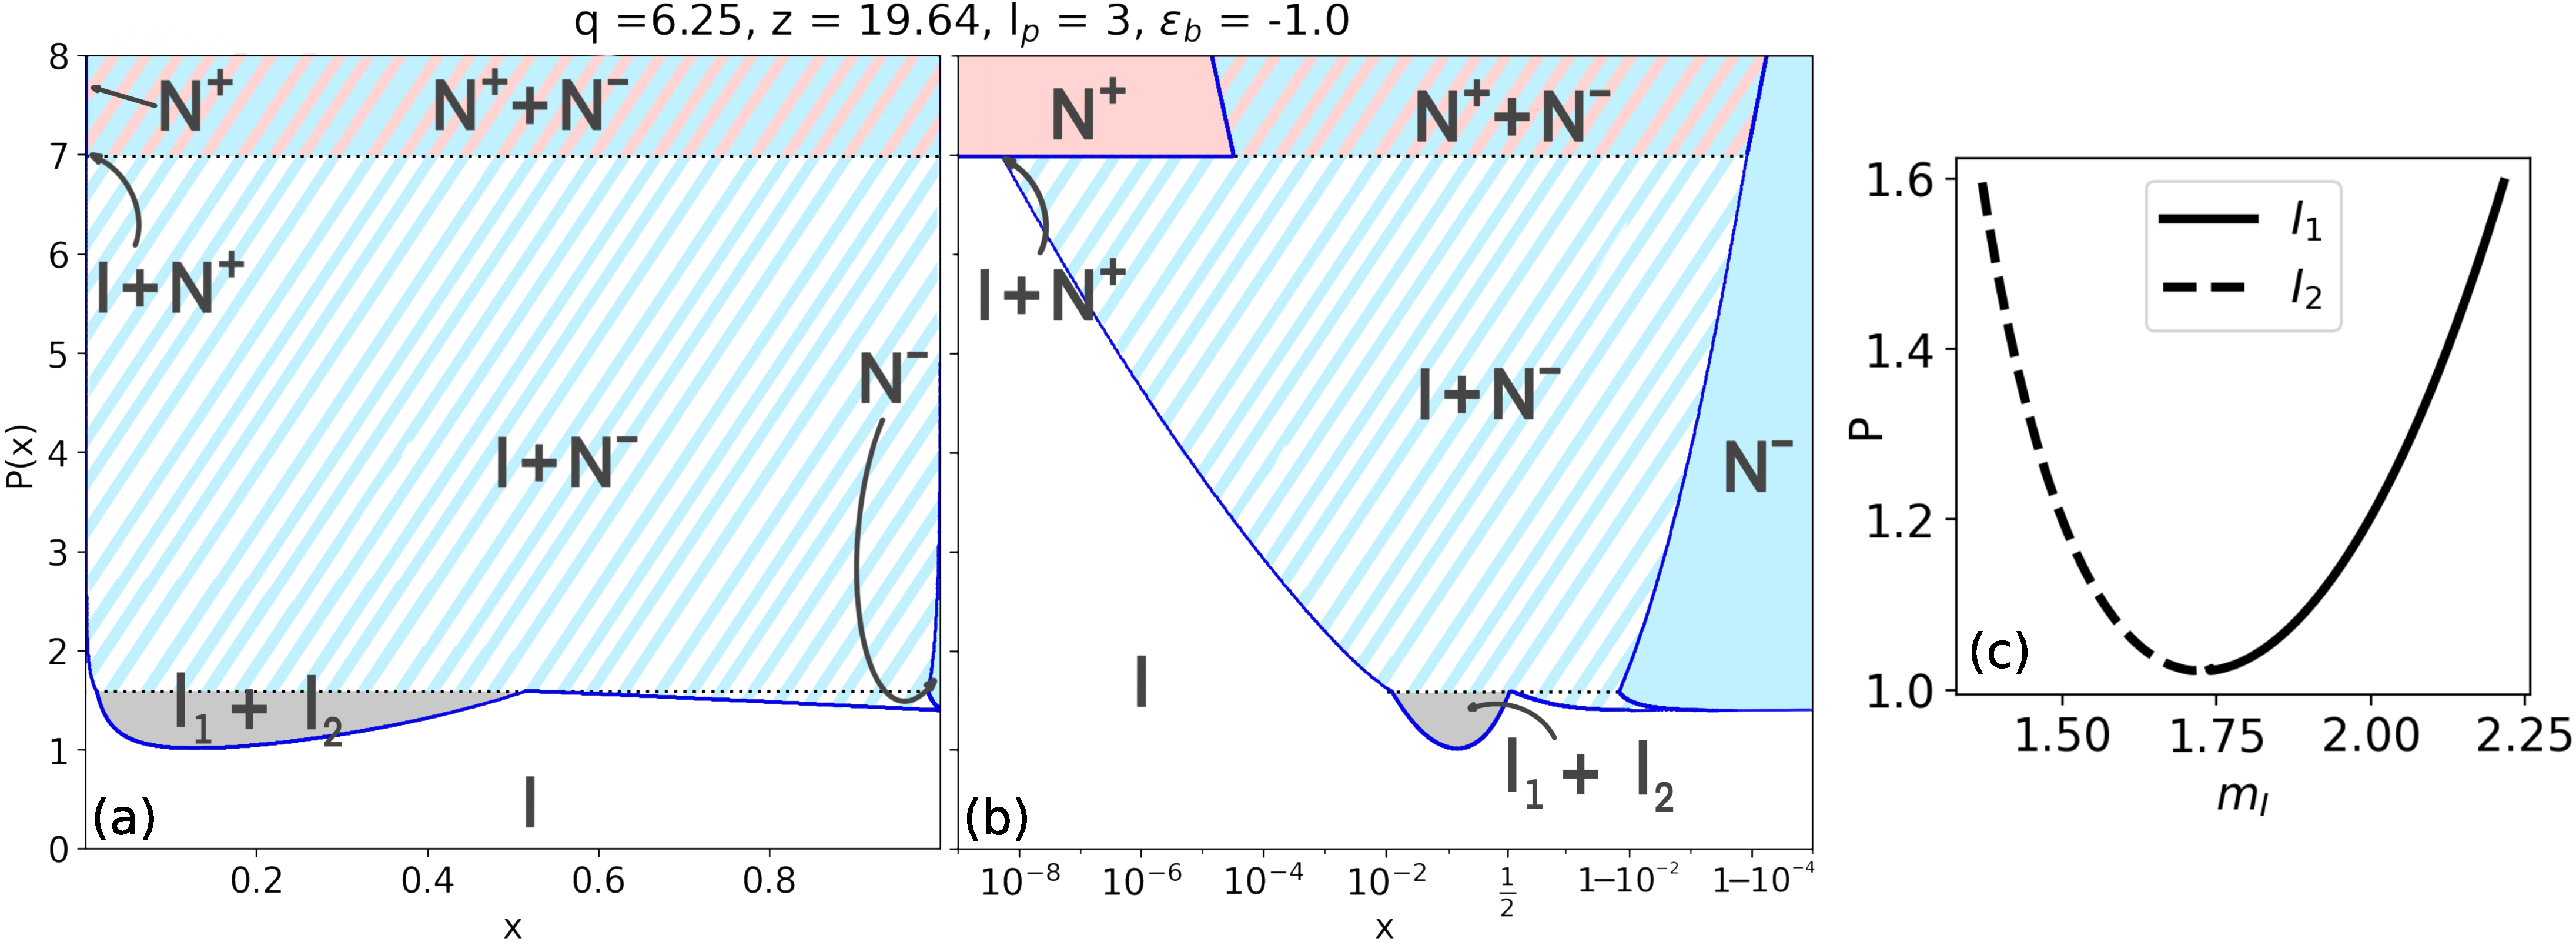
\includegraphics[width= \linewidth]{figures/chapter-3/FIG5}
\caption{Phase diagram in the osmotic pressure-composition ($P-x$) representation with the following parameters: persistence length $\ell_{p} = 3$, effective temperature $\varepsilon_{b} = -1$, excluded-volume {\em ratios} $q = \frac{1}{4}\frac{L_{r}}{D_{r}}$ and $z=\pi q$ corresponding to a monomer aspect ratio $L_{r}/D_{r} =25$. The disc mole fraction $x$ is plotted on a linear scale (a) and on a logarithmic scale (b) to highlight the behavior close to single-component systems (pure polymers $x=0$, and pure discs $x=1$). Note the presence of a coexistence between an isotropic gas and fluid  phase ($I_1$ and $I_2$) with different discs compositions (grey region). (c) Comparison of mean aggregation numbers $m_{I}$ between $I_{1}$ and $I_{2}$ for a given pressure. $I_{1}$ corresponds to the phase at the lowest disc mole fraction $x$. }
  \label{fig:coexistence}
\end{figure*}

We move on to explore a similar mixture featuring more slender rod monomers, namely $L_{r}/D_{r} = 25$. The resulting phase diagram is shown in \fig{fig:coexistence}. The asymmetry of the mixture is now very strong with the monophasic  $N^{+}$ and $N^{-}$ regions being largely unstable except for strongly purified systems  ($x$ close to $0$ or $1$)  [\fig{fig:coexistence}(b)]. Qualitatively, the phase diagram resembles the one in \fig{fig:L10}(a), but the isotropic fluid  undergoes a gas-liquid-type phase separation producing two phases differing in composition. The $I_{1}$-phase may be associated with a discotic colloidal gas, and  $I_{2}$  with its liquid counterpart.   The demixing is driven by the extreme excluded-volume difference between the rod monomers and the discs. This phenomenon has been reported for (non-polymerizing) rod-disc mixtures in Ref. \cite{varga2002}, where the effect was ascribed to a {\em depletion} of discs by the much smaller rods. Isotropic-isotropic demixing has  been more generally observed when mixing different shapes dominated by hard-core repulsion \cite{dijkstra1994}, including thin and thick rods \cite{vanRoij97}, spheres and discs   \cite{chen2015,aliabadi2016} and discs  differing in diameter \cite{phillips_pre2010}. It has also been observed in thermotropic LC-solvent mixtures where the effect is primarily of enthalpic origin and is caused by specific interactions between the LC forming molecules and the solvent \cite{matsuyama1996,reyes2019}.  It is well known that mixing colloids with non-adsorbing polymer depletants creates an effective attraction between the colloids which is entirely of entropic origin and may drive various types of demixing mechanisms \cite{LekkerkerkerTuinier2011}. In our case, the depletion effect is however less clear-cut given that the ``depletants"   reversibly polymerize into a wide array of different sizes \cite{peters2021} and experience  orientation-dependent volume-exclusion interactions which are usually ignored in colloid-polymer models. Moreover the average polymer size depends, via \eq{miso}, on the monomer concentration which is different in the gas and liquid phases. \fig{fig:coexistence}(c) demonstrates that the difference in mean aggregation number between the two isotropic phases is in fact quite small, with the disc-rich fraction harboring slightly longer polymers.   Note that the presence of isotropic-isotropic demixing gives rise to a low-pressure triple equilibrium where both phases coexist with a discotic nematic $N^{-}$.  

\section{Quadruple fluid coexistence}

% TODO: central alignment
\begin{figure*}[ht]
  \includegraphics[width=0.8 \linewidth]{figures/chapter-3/FIG6}
\caption{(a) Phase diagram in the osmotic pressure-composition ($P-x$) representation showing an $I_{1}$-$I_{2}$-$N^{+}$-$N^{-}$ quadruple point at $P = 4.29$. For this particular case, $\ell_{p} = 3$, $\varepsilon_{b} = -1.2$, $L_{r}/D_{r} =25$ and $D_{d}/L_{r} = 0.7$. (b) Visualization of combinations of rod-disc excluded-volume ratio ($q$ and $z$) and temperature $\varepsilon_{b}$ where  an $I_{1}-I_{2}-N^{+}-N^{-}$ quadruple coexistence is possible.  }
\label{fig:qp}
\end{figure*}

At this stage, one might wonder whether a mixtures could be designed in which  the two separate triple equilibria  in \fig{fig:coexistence} were to join into a  {\em quadruple} coexistence featuring all fluid phases. In \fig{fig:qp}(a) we demonstrate that this scenario is indeed possible. For the particular mixture shown there, the rod monomers and discs no longer have equal largest dimensions ($L_{r}= D_{d}$) but the disc diameter is somewhat smaller than the rod length, namely $D_{d} =0.7 L_{r}$ while the rods are kept sufficiently slender ($L_{r}/D_{r} = 25$). The  excluded-volume asymmetry is then sufficiently reduced to make the two triple points coincide and generate a simultaneous coexistence between two isotropic and two nematic phases, each differing in monomer-disc composition and overall particle concentration. This mixture is by no means  unique and belongs to a family of monomer-disc size ratios where a remarkable $I_{1}$-$I_{2}$-$N^{+}$-$N^{-}$ quadruple point could be encountered, as illustrated by the colored manifold in \fig{fig:qp}(b). This result provides important guidance if one wishes to explore these intricate multi-phase equilibria in real-life mixtures featuring reversibly polymerizing rods mixed with colloidal platelets.

 At this point we wish to draw a connection with recent theoretical explorations of polymer depletion on purely monomeric colloidal rods which have revealed similar multi-phase equilibria involving one-dimensional periodic smectic structures as well as fully crystalline states \cite{peters_prl2020}. Similar phenomena involving isotropic-nematic-columnar quadruple points had been reported previously for disc-polymer mixtures \cite{gonzalez2017}. In those studies, the multiphase equilibria emerge from an effective one-component theory based on free-volume theory where   polymeric depletants, envisaged as fixed-shape spherical particles that do not interact with one another, are depleted from the surface of the colloidal rod due to volume exclusion as per the original Asakura-Oosawa model \cite{ASAKURA54,ASAKURA58,Vrijdepletie}. In our work, the depletion effect is strongly convoluted since all components (polymer species and discs alike) are explicitly correlated, albeit on the simplified second-virial level. Furthermore, high-density crystal phases with long-ranged positional order are not considered in the present study since their stability requires strong uniformity in particle shape \cite{mederos_overview2014}, which is not the case in our mixtures. In fact, even for basic mixtures of non-associating hard rods mixed with hard discs the full phase behavior at conditions of elevated particle packing  remains largely elusive to this day. Large-scale  numerical simulations or density-functional computations are needed  to overcome the limitations of the simple second-virial approach taken here, but these are technically challenging to implement for dense multi-component systems. 
 
 The results gathered in \fig{fig:qp}  illustrates the possibility of generating four different fluid textures emerging from reversibly changing excluded-volume-driven interactions alone, without the need to invoke attractive interparticle forces. This could bear some relevance on the emergence of functionality through liquid-liquid type phase separation in biological cells which are composed of biomolecules possessing a multitude of different shapes, some of them  controlled by reversible association \cite{hyman2014,shin2017}.
 
 % TODO: transfer to general conclusions??
\section{Conclusions}

We have explored the phase behaviour of a simple model for thermoresponsive supramolecular rods mixed with discotic particles. Possessing attractive tips the rod monomers reversibly associate into polymers that retain their basic slender rod shape and experience only a limited degree of backbone flexibility. The interaction between the species is assumed to be  of steric origin such that basic shape differences between the constituents, more specifically the excluded-volume disparity, plays a key role in determining the prevailing liquid crystal symmetry. The principal ones are a   polymer nematic ($N^{+}$) composed of nematic polymer interspersed with an anti-nematic organization of discs and a discotic nematic  ($N^{-}$) in which the polymers are dispersed anti-nematically.   Lowering   temperature stimulates  polymer growth which  enlarges the stability window for the $N^{+}$ phase.  The phase diagram  develops a marked {\em azeotrope} upon increasing the mole fraction of added discs which indicated that the  polymer nematic is stabilized by the addition of non-adsorbing rigid discs provided their mole fraction remains small. 
The polymer-dominated nematic phase eventually becomes destabilized at larger mole fractions where mutual disc alignment disrupts  the nematic  order of the polymers in favour of the formation of a discotic nematic phase in which the polymers self-organize into an anti-nematic structure. The corresponding molecular weight distribution functions strongly deviates from the usual exponential form and becomes non-monotonic with a maximum probability associated with oligomeric aggregates. Enhancing the shape-asymmetry between the rod monomers and discs we observe a depletion-driven demixing of the isotropic fluid which opens up the possibility of a quadruple existence featuring two isotropic phase along with the fractionated polymer and discotic nematic phases. Such quadruple points occur in a wide range of mixed-shape nematics involving supramolecular rods templated by discs and highlight the possibility of multiple liquid symmetries (both isotropic and anisotropic) coexisting in  mixtures of anisotropic colloids with reversible and thermoresponsive shape-asymmetry without cohesive interparticle forces.   Future explorations should aim at a more careful assessment of biaxial nematic order, ignored in the present study,  which could develop in near-equimolar rod-disc mixtures provided they are stable against global demixing (see Appendix B for tentative discussion). Polymerizing rods and discs with finite particle thickness and low shape asymmetry may favor the emergence of liquid crystals possessing lamellar, columnar or fully crystalline signatures  \cite{peroukidis2010} which may be addressed using  computer simulation models along the lines of Refs. \cite{kuriabova2010,nguyen2014,perouklapp2020}. Inspiration for such mixed-shape  lamellar structures  could be drawn from bio-inspired supramolecular liquid crystals \cite{safinya2013} such as, for example, the `sliding columnar phase' and similar stacked architectures  observed in cationic lyposome-DNA complexes \cite{wong2000,ohern1998} which are essentially made up of mixed planar and rod-shaped architectures. 

% TODO: transfer to general appendices
\section*{Appendix A: Renormalized ${\mathcal P}_{2}$ approximation for slightly flexible polymers}

We seek a simple perturbation theory for the one-body density   \eq{lnrhor}  of near-rigid polymers characterized by a finite persistence length $\ell_{p}$. Let us attempt the following generalization of the probability density distribution for the polymers: 
\beq
 \rho_{r} (\ell , \oma) =  \ell e^{\varepsilon_{b} + \lambda_{r} \ell} e^{ \ell (a_{r}+ \xi) \pp(\oma) }
\eeq
with $\xi$ representing a correction induced by the {\em internal} orientational entropy of the polymer due to a small degree of worm-like chain flexibility. 
Inserting this expression into the worm-like chain contribution (last term) in the EL equation  \eq{lnrhor},  substituting $\nabla^{2} = \partial_{t} (1-t^{2}) \partial_{t}$ and $t= \cos \theta$,  we find that for the uniaxial symmetry:
\begin{align}
\frac{\nabla^{2}  \rho_{r}^{1/2}}{  \rho_{r} ^{1/2} }  = & \frac{3}{4} \tilde{a}_{r}^{2} + \left  ( \frac{3}{2}  \tilde{a}_{r} ^{2}  - 3 \tilde{a}_{r} \right ) \pp(t) + {\mathcal O}(t^{4})
\label{roro1}
\end{align}
where $\tilde{a}_{r} = a_{r}  + \xi$ denotes a rescaled alignment amplitude for the polymer. 

\subsection*{Anti-nematic polymers}
We expect that neglecting the fourth-order term will be fairly harmless in a strongly anti-nematic state  where $t $ is generally very small (since $\theta \sim \pi/2 $ for most polymers). This situation is naturally encountered in the  $N^{-}$ phase where $a_{r} \ell \ll 0 $ in particular for the long polymers.  The constant  in \eq{roro1} is unimportant for the EL equation where it can be subsumed into the normalization factor $\lambda$, but must be retained when computing the worm-like chain free energy. Then, consistency requires that
\beq
\xi \approx  \frac{1}{3 \ell_{p}}  \left  ( \frac{3}{2}  \tilde{a}_{r} ^{2}  - 3 \tilde{a}_{r}  \right )
\eeq 
where the chain persistence length $\ell_{p}$ should be interpreted in units of the segment length $L_{r}$.  From the above the dependence of $\xi$ on the bare alignment amplitude $a_{r}$ is easily resolved and we find:
 \beq
 \xi \approx 1+ \ell_{p} +   |a_{r} |  -\sqrt{(1 +  \ell_{p})^{2} + 2 | a_{r} |  \ell_{p} }, \hspace{0.3cm} (a_{r} \ll 0 )
 \label{xi1}
 \eeq 
The correction factor vanishes in the rigid rod limit, $\lim_{\ell_{p} \rightarrow \infty} \xi = 0$, as it should.

\subsection*{Nematic polymers}

We may repeat the analysis for the case of conventional nematic polymers as encountered in the polymer-dominated $N^{+}$  phase using a slightly different route. For $a_{r} \gg 1$ the average polar deflection angle will be small and we may expand the worm-like chain term up to quadratic order in $\theta$. Using the asymptotic relation $\pp(t) \sim 1- 3\theta^{2}/2 $ and ignoring any constant factors we find a simple approximation valid for $|t|$ close to unity (strong alignment): 
\begin{align}
\frac{\nabla^{2}  \rho_{r}^{1/2}}{  \rho_{r} ^{1/2} }  \sim - \frac{3}{2} (  \tilde{a}_{r} ^{2}  + 2  \tilde{a}_{r} ) \pp(t) 
\label{roro2}
\end{align}
Then, in analogy with the preceding case we find an expression identical to \eq{xi1} except for a minus sign:
\beq
 -\xi \approx 1 + \ell_{p} + |a_{r}|  - \sqrt{(1 +  \ell_{p})^{2} + 2 |a_{r}|  \ell_{p}}, \hspace{0.3cm} (a_{r}  \gg 0)
\label{xi2}
\eeq
 This simple scaling result confirms our expectation, namely that a small degree of backbone flexibility leads to a reduction of the alignment propensity of the polymers, since $| a_{r} + \xi | $ is always smaller than $| a_{r}  |$. For strongly aligned systems, this effect turns out to be of equal strength for both nematic and anti-nematically ordered polymers.
 



% TODO: transfer to general appendices
\section*{Appendix B: Stability of biaxial nematic order}

% TODO: central alignment
\begin{figure*}[ht]
  \includegraphics[width=.8 \textwidth]{figures/chapter-3/FIG7}
\caption{(a) Schematic representation of the biaxial nematic phase $BX$ with orthorhombic ($D_{2h}$) point-group  symmetry, characterized by mutually perpendicular nematic directors for each species ($\bm{\hat{\textnormal{\bfseries n}}_r}$ for the polymers and $\bm{\hat{\textnormal{\bfseries n}}_d}$ for discs). (b) Bifurcation curves locating the transition from uniaxial (U) order at low osmotic pressure $P$ to biaxial (BX) nematic order at high pressure for a number of relevant cases studied in the main text. Here, $x$ denotes the disc mole fraction.  }
\label{fig:bx}
\end{figure*}



So far, we have overlook the possibility of biaxial nematic order in which both polymers and discs order along mutually perpendicular directors (see \fig{fig:bx}(a)).
In order to tentatively locate the transition toward biaxial ($BX$) nematic order, we  apply a simple bifurcation analysis in which we probe the stability a uniaxial ($U$) fluid against weakly biaxial fluctuations \cite{kayser,stroobants1984}. If the $U$-$BX$ transition is second-order, the bifurcation point at which biaxial solution emerge from the EL equations should pinpoint the actual phase transition.  We begin by generalizing the second-polynomial expansion \eq{p2expansion} to include biaxial nematic order using the addition theorem for spherical harmonics:
\begin{align}
\pp( \cos \gamma ) &= \pp(\cos \theta) \pp(\cos \theta^{\prime})  \nonumber \\ 
& + \frac{1}{12} \pp^{2}(\cos \theta) \pp^{2}(\cos \theta^{\prime}) \cos 2 (\varphi - \varphi^{\prime})
\end{align}
where $\varphi$ is the azimuthal angle describing the particle orientation  with respect a secondary director $\bn_{\perp} \perp \bn$. The coupled EL equations then attain an additional term that accounts for biaxiality: 
\begin{align}
&  \ell^{-1} \ln [  \rho_{r} (\ell, \oma ) \ell^{-1} ]   = \lambda_{r}    + \varepsilon_{b}  +  \alpha_{r}  \pp(\oma ) \nonumber \\ 
& +  \beta_{r } D(\oma)   +  \frac{L_{r}}{3\ell_{p}} \frac{\nabla^{2} [ \rho_{r} (\ell , \oma)]^{1/2}}{ [ \rho_{r} (\ell , \oma)]^{1/2} }
\label{lnrhorbiax}
\end{align}
and
\begin{align}
\ln [  \rho_{d} (\oma )] & = \lambda_{d}  + \alpha_{d} \pp(\oma)  + \beta_{d} D(\oma )  
\label{lndbiax}
\end{align}
in terms of the  weight function $D(\oma) = \sin^{2} \theta  \cos 2 \varphi $ and amplitudes: 
\begin{align}
\beta_{r} &=  \frac{15 }{16}  ( \rho_{r0} \bar{\Delta}_{r}  - 2q  \rho_{d0}  \Delta_{d} )  \nonumber \\
\beta_{d} &=   \frac{15 }{16}  (z \rho_{d0}  \Delta_{d}  - 2 q \rho_{r0}  \bar{\Delta}_{r} )
\label{alphabetabiax}
\end{align}
which feature the biaxial nematic order parameter of each species:
\begin{align}
\Delta_{r \ell} &= \rho_{r \ell}^{-1} \int d \oma \rho_{r}(\ell, \oma) D (\oma) \nonumber \\
\Delta_{d} &= \rho_{d0}^{-1} \int d \oma \rho_{d}( \oma) D (\oma ) 
\label{dr}
\end{align}
Similar to the uniaxial case the bar denotes a molecular-weight average according to $ \bar{\Delta}_{r} = \rho_{r0}^{-1}  \sum_{\ell} \rho_{r\ell} \Delta_{r \ell}$. 
Substituting the EL equations  into the  biaxial nematic order parameters and linearize for weakly biaxial amplitudes $|\beta| \ll 1$ we establish the condition under which a biaxial solution for the orientation distribution bifurcates from the uniaxial  one:
\begin{align}
\Delta_{r \ell} &= \rho_{r \ell}^{-1} \ell \beta_{r} \int d \oma \rho_{r }^{(U)} ( \ell, \oma) D^{2} (\oma) \nonumber \\
\Delta_{d} &= \rho_{d0}^{-1}  \beta_{d} \int d \oma \rho_{d }^{(U)} (\oma) D^{2} (\oma)
\label{brod}
\end{align} 
This linear criterion basically stipulates the conditions (overall particle concentration, composition and effective temperature) at which the  uniaxial nematic state is no longer guaranteed to be a local minimum in the free energy. Within the factorization Ansatz \eq{pfac} for the uniaxial molecular-weight distributions the condition simplifies into:
\begin{align}
\bar{\Delta}_{r} &=  \beta_{r} (2 m-1)  \langle D^{2}  (\oma) \rangle_{f_{G}} \nonumber \\
\Delta_{d} &=   \beta_{d}  \langle D^{2}  (\oma) \rangle_{f_{G}}
\label{brodgauss}
\end{align} 
The brackets denote an average according to the nematic or anti-nematic Gaussians  $f_{G}$ specified in \eq{gaussians}. Similarly, $m$ denotes the mean aggregation number of either the $N^{+}$ or the $N^{-}$ phase.
The averages are easily obtained in the asymptotic angular limits ($\theta \ll 1$ or $\psi \ll 1$) and the leading order contributions read:
\beq
\langle D^{2}  (\oma) \rangle_{f_{G}}  \sim 
 \begin{cases}
 4 /[ \alpha^{(1)}]^{2} \hspace{0.5cm}  \textrm{nematic}  \\
1/2 \hspace{1.2cm}   \textrm{anti-nematic} 
\end{cases}
\eeq 
 The $U$-$BX$ bifurcation condition \eq{brodgauss} is equivalent to the matrix equation ${\bf M} \cdot {\bf \Delta}  = \lambda_{e} {\bf \Delta} $ with ${\bf \Delta} = ( \bar{\Delta}_{r} , \Delta_{d}) $ and ${\bf M}$ given by the prefactors.  The eigenvalues $\lambda_{e} $ of the matrix ${\bf M}$ are required to be unity $(\lambda_{e} =1)$. The solution is:
 \begin{align}
 1 &= -\frac{15}{32} c w_{1} \left[ (1-x) + xzW - \right . \nonumber \\ 
 & \left . \sqrt{(1-x)^{2} + 2Wx(1-x)(8 q^{2} -z) +W^{2} x^{2}z^{2} }  \right]
\end{align}
with
\beq
w_{1} = 
 \begin{cases}
 (2m_{N^{+}}-1) 4/\alpha_{r}^{2}  \hspace{0.5cm}  N^{+}-BX  \\
 (2m_{N^{-}}-1)/2 \hspace{0.7cm}  N^{-}-BX
\end{cases}
\eeq 
and
\beq
W = 
 \begin{cases}
 (2m_{N^{+}}-1)^{-1} \alpha_{r}^{2}/8  \hspace{0.5cm}  N^{+}-BX  \\
 (2m_{N^{-}}-1)^{-1} 8/\alpha_{d}^{2} \hspace{0.5cm}  N^{-}-BX
\end{cases}
\eeq 

The numerical solutions are shown in \fig{fig:bx}(b).  The $N^{-}$-$BX$ solutions ceases to be internally consistent with the Gaussian approximation at  $x< 0.8$ given that the nematic order parameter $\alpha_{d}$ of the discs tends to get too low. No such inconsistency occurs for the $N^{+}$-$BX$ branches. In general, we find that the transition occurs at pressures that are beyond the ranges explored in the phase diagrams of the main text. The only exceptions are \fig{fig:L10}(c) and \fig{fig:qp} where the $N^{+}$ phase remains stable up to fairly large disc mole fractions and the $N^{+}$-$BX$ bifurcations are located within the monophasic $N^{+}$ regions (in red). The tentative conclusion from this analysis is in line with previous reports in literature \cite{mederos_overview2014}, namely that the stability of $BX$ nematic order is intimately linked to the excluded-volume asymmetry of the constituents which, in our case, is temperature-controlled.  Lowering the temperature reduces the typical asymmetry which then stabilizes well-mixed rod-disc nematics that subsequently may develop $BX$ order. We further note that disc-rich $BX$ phases seem much harder to stabilize than polymer-dominated ones as the $N^{-}$-$BX$ branches  generally do not intersect the small monophasic $N^{-}$ domains in the phase diagrams shown in the main text. 

 





\clearpage % Disk-polymers

\chapter{Bi-helical order and demixing in hybrid chiral LCs}
\chaptermark{Hybrid LCs: correlation effects}
\label{hybridLC2}


\begin{abstract}

We extend Onsager's theory to the case of hybrid molecular liquid crystals (LC) composed of colloidal particles immersed in thermotropic host. This framework enables us to explore colloid concentrations that are no longer infinitely small. Correlations between the colloids cause additional entropic and elastic contributions that interfere with surface anchoring effects explored in the previous chapter.  We consider two distinct regimes, namely weak coupling where surface anchoring only marginally impacts the colloid orientations and strong coupling where the typical realignments energy strongly exceeds the thermal energy. We demonstrate at weak coupling that collective colloidal effects driven by steric colloid-colloid interaction may lead to liquid-liquid phase separation between two biaxial fluid phases. In the strong coupling regime, we argue that elastic force may facilitate the formation bi-helical states where the helical organization of the colloidal and molecular components is unequal in pitch and even in handedness. 

\end{abstract}



\section{Introduction}

In the previous chapter we have studied  ordering of colloidal particles in so-called hybrid chiral liquid crystals composed of colloidal particles immersed in a low-molecular-weight cholesteric LC. Inspired by experimental work of we restricted our attention to the regime of low colloidal content where the principal ordering effect stem from single colloid properties related to surface anchoring and elastic distortions formed around the colloid surface. In this regime,  the average interparticle distance remains sufficiently large to guarantee that direct interactions between colloids, mediated by steric collisions or guided by some interference of surface defects, is unimportant. Raising the concentrations of colloids, which has not  been pursued in experiment thus far, offers interesting perspectives to explore the interplay between surface anchoring and alignment driven by colloid-colloid interactions as well as the role of (twist) elastic forces imparted by steric correlations between the colloids. In this chapter we generalize Onsager's theory suitably adapted to treat spatially non-uniform director field such as in a cholesteric, to explore the ordering of colloids at large concentrations where entropic and elastic contributions imparted by the colloids play a role. In doing so we consider two extreme cases, namely weak coupling where colloid realignemt cause by surface anchoring forces is weak, and strong coupling where such realignment is strong compared to the typical thermal fluctuations the colloid experience.  We highlight two main effects (i) surface-anchoring-driven  phase separation between two orthorhombic liquids at weak surface anchoring coupling and (ii) the formation of bi-helical chiral hybrid liquid crystals at large coupling strength.  Since the latter case should occur for both rods and discs alike exploring mixed molecular-colloidal LCs with inherent chirality opens up ways to create chiral fluids composed of discotic mesogens \cite{bisoyi2010discotic,bushby2002discotic}.   



\section{Second-virial density functional }

 With the single-colloid properties fully specified in the previous chapter, we now proceed towards describing the many-particle system by invoking a simple Onsager-type density functional theory \cite{Onsager}. The grand potential $\Omega$ of an assembly of colloids in the presence of an external  potential  reads in general form \cite{allenevans}:
 \begin{align}
 &  \Omega[\rho ]  = \int d \bfr d \bhu  \rho(\bfr, \bhu) \left [k_{B}T \ln {\mathcal V}   \rho(\bfr, \bhu)  +   U_{\rm ext}(\bfr, \bhu) - \mu  \right ] \nonumber \\
 & -\frac{k_{B}T}{2} \int d \bfr d \bhu \int d \bfr^{\prime} d \bhu^{\prime}  \rho(\bfr, \bhu)  \rho(\bfr^{\prime}, \bhu^{\prime}) \Phi(|\bfr - \bfr^{\prime}|, \bhu, \bhu^{\prime} )
 \label{grandpot}
 \end{align}
 with ${\mathcal V}$ denoting an effective thermal volume comprising contributions from rotational momenta and $\mu$ a chemical potential that controls the overall colloid concentration.  The first contribution describes an ideal gas of  non-interacting colloids while the second accounts for colloid-colloid interaction on the second-virial level. Here, the key input is the Mayer function $\Phi$  that, assuming the colloid interactions to be purely hard, renders minus unity if the cores of two colloids overlap and zero if they do not.

 We assume that the colloid positions remain randomly distributed. The orientational probability, however, will be affected by a helical rotation of  the  colloidal director field $\bn(z)$. Since the cholesteric pitch $\lambda \approx 30 \mu m$ is about an order of magnitude larger than the typical colloidal size (a few $\mu m$), the colloidal director is completely enslaved to the rotation of the local cholesteric director and adopts the same pitch length $\lambda$. A $\pi/2$ phase shift between the colloidal director $\bn(z)$ and the cholesteric one $\bn_{s}(z)$ may occur under certain anchoring conditions as we observe in Figs. 1 and 2.  This scenario may no longer hold at larger colloid concentrations and/or shorter cholesteric pitches where the twist elasticity of the colloids becomes considerable, as we will contemplate in a later section. Let us proceed by parameterizing the one-body density in terms of an overall density $\rho = N/V$ and an orientational probability that explicitly depends on the position $z$ along the helix:
 \beq
  \rho(\bfr, \bhu) = \rho f_{q}(\bhu \cdot \bn(z))
 \eeq
 In order to elaborate the grand potential we parameterize the system volume in cylindrical coordinates $d \bfr  = d \bfr_{\perp} dz$ with $0< |r_{\perp}| < \infty$ and $0< z < 2 \pi/q$. Given that the overall rod density is prescribed, the grand potential becomes a Helmholtz free energy $F$. The ideal (translation plus orientation) entropy  free energy per unit volume follow from:
  \begin{align}
 & \frac{ \beta F_{\rm id}}{ V} =  \int d \bhu \int_{0}^{2\pi}  \frac{d(qz)}{2 \pi} f_{q}( \bhu \cdot \bn(z))  \ln [{\mathcal V} \rho  f_{q}( \bhu \cdot \bn(z))]
 \end{align}
Since the orientational distribution does not change along the cholesteric director the ideal free energy density simplifies into the conventional form:
 \begin{align}
  \frac{ \beta F_{\rm id}}{ V} =  \rho \int d \bhu \ln [{\mathcal V} \rho  f_{q}( \bhu \cdot \bn)] f_{q}( \bhu \cdot \bn)
 \end{align}
 with $\bn$ denoting the local director along the helix. Similarly, the external potential in \eq{grandpot} is associated the surface anchoring free energy obtained from the Rapini-Papoular expression \eq{usurf}. It is  defined in the angular coordinates $\bhu(\theta, \delta)$ that co-rotate with the helical director so that:
\beq
\frac{F_{\rm s}}{V} = \rho \int d \bhu   f_{q}(\bhu \cdot \bn)  F_{s}(\bhu)
\eeq
Next, we introduce a linear coordinate transformation $z^{\prime} = z + \Delta z$ and write the excess free energy as follows:
  \begin{align}
  \frac{ \beta F_{\rm ex}}{ V}  = & \frac{\rho^{2}}{2} \int_{0}^{2 \pi}  \frac{d(qz)}{2 \pi}  \int d \bhu \int d \bhu^{\prime}  f_{q}( \bhu \cdot \bn(z)) \nonumber \\
  & \times \int_{-\lambda}^{\lambda} d \Delta z  {\mathcal A}(|\Delta z | , \bhu, \bhu^{\prime} ) f_{q}( \bhu^{\prime} \cdot \bn(z+\Delta z))
 \end{align}
 where  ${\mathcal A}$  is an orientation-dependent excluded {\em area} of rod or disc. The excess free energy is non-local since it depends on volume exclusion between a reference particle at $z$ and test particle  at $z+ \Delta z$ over which the local director will have rotated. It is therefore expedient to apply a transformation $\bhu^{\prime} \rightarrow \mathcal{R} (q\Delta z) \bhu^{\prime}$  which projects the orientation of the test colloid into the director frame of the reference one located at $z$ via the rotation matrix:
 \beq
 \mathcal{R} (q\Delta z)   =
  \begin{bmatrix}
     \cos(q\Delta z)  & \sin(q\Delta z) & 0   \\
   - \sin(q \Delta z) & \cos(q\Delta z) & 0  \\
   0 & 0 &  1  \\
      \end{bmatrix}  \nonumber
      \label{rota}
 \eeq
 The renders the excess free energy local so that it may be simplified into a compact form:
 \begin{align}
  \frac{ \beta F_{\rm ex}}{ V}  = & \frac{\rho^{2}}{2} \int d \bhu \int d \bhu^{\prime}  f_{q}( \bhu \cdot \bn) f_{q}( \bhu^{\prime} \cdot \bn) {\mathcal K}_{q}(\bhu, \bhu^{\prime})
 \end{align}
in terms of and excluded volume that takes into account the helical rotation of the director field:
\beq
 {\mathcal K}_{q}(\bhu, \bhu^{\prime}) =  \int_{-\lambda }^{\lambda} d \Delta z {\mathcal A}(|\Delta z | , \bhu, \mathcal{R}(q\Delta z)  \bhu^{\prime} )
\eeq
This clearly represents a highly convoluted object that we were only able to analyze analytically for thin hard rods, as discussed in the Appendix.
 As alluded to before, in the experimental situation the director twist is weak on the scale of the typical colloid size and it is justified to assume
\beq
 {\mathcal K}_{q}(\bhu, \bhu^{\prime}) \approx {\mathcal K}_{0}(\bhu, \bhu^{\prime}) =  v_{0}| \sin \gamma|
\eeq
which corresponds to the conventional excluded volume between two (infinitely) thin hard rods ($v_{0} = 2 L^{2}D$) or discs ($v_{0} = \tfrac{\pi}{2}D^{3}$), as per Onsager's original theory \cite{Onsager}. This approximation ignores any twist elastic resistance imparted by the colloids and should hold only for low to moderate colloid concentrations and weak director twist ($\lambda \gg L$ or $D$).  The effect of finite twist elasticity will be considered in an upcoming Section.


\begin{figure}
	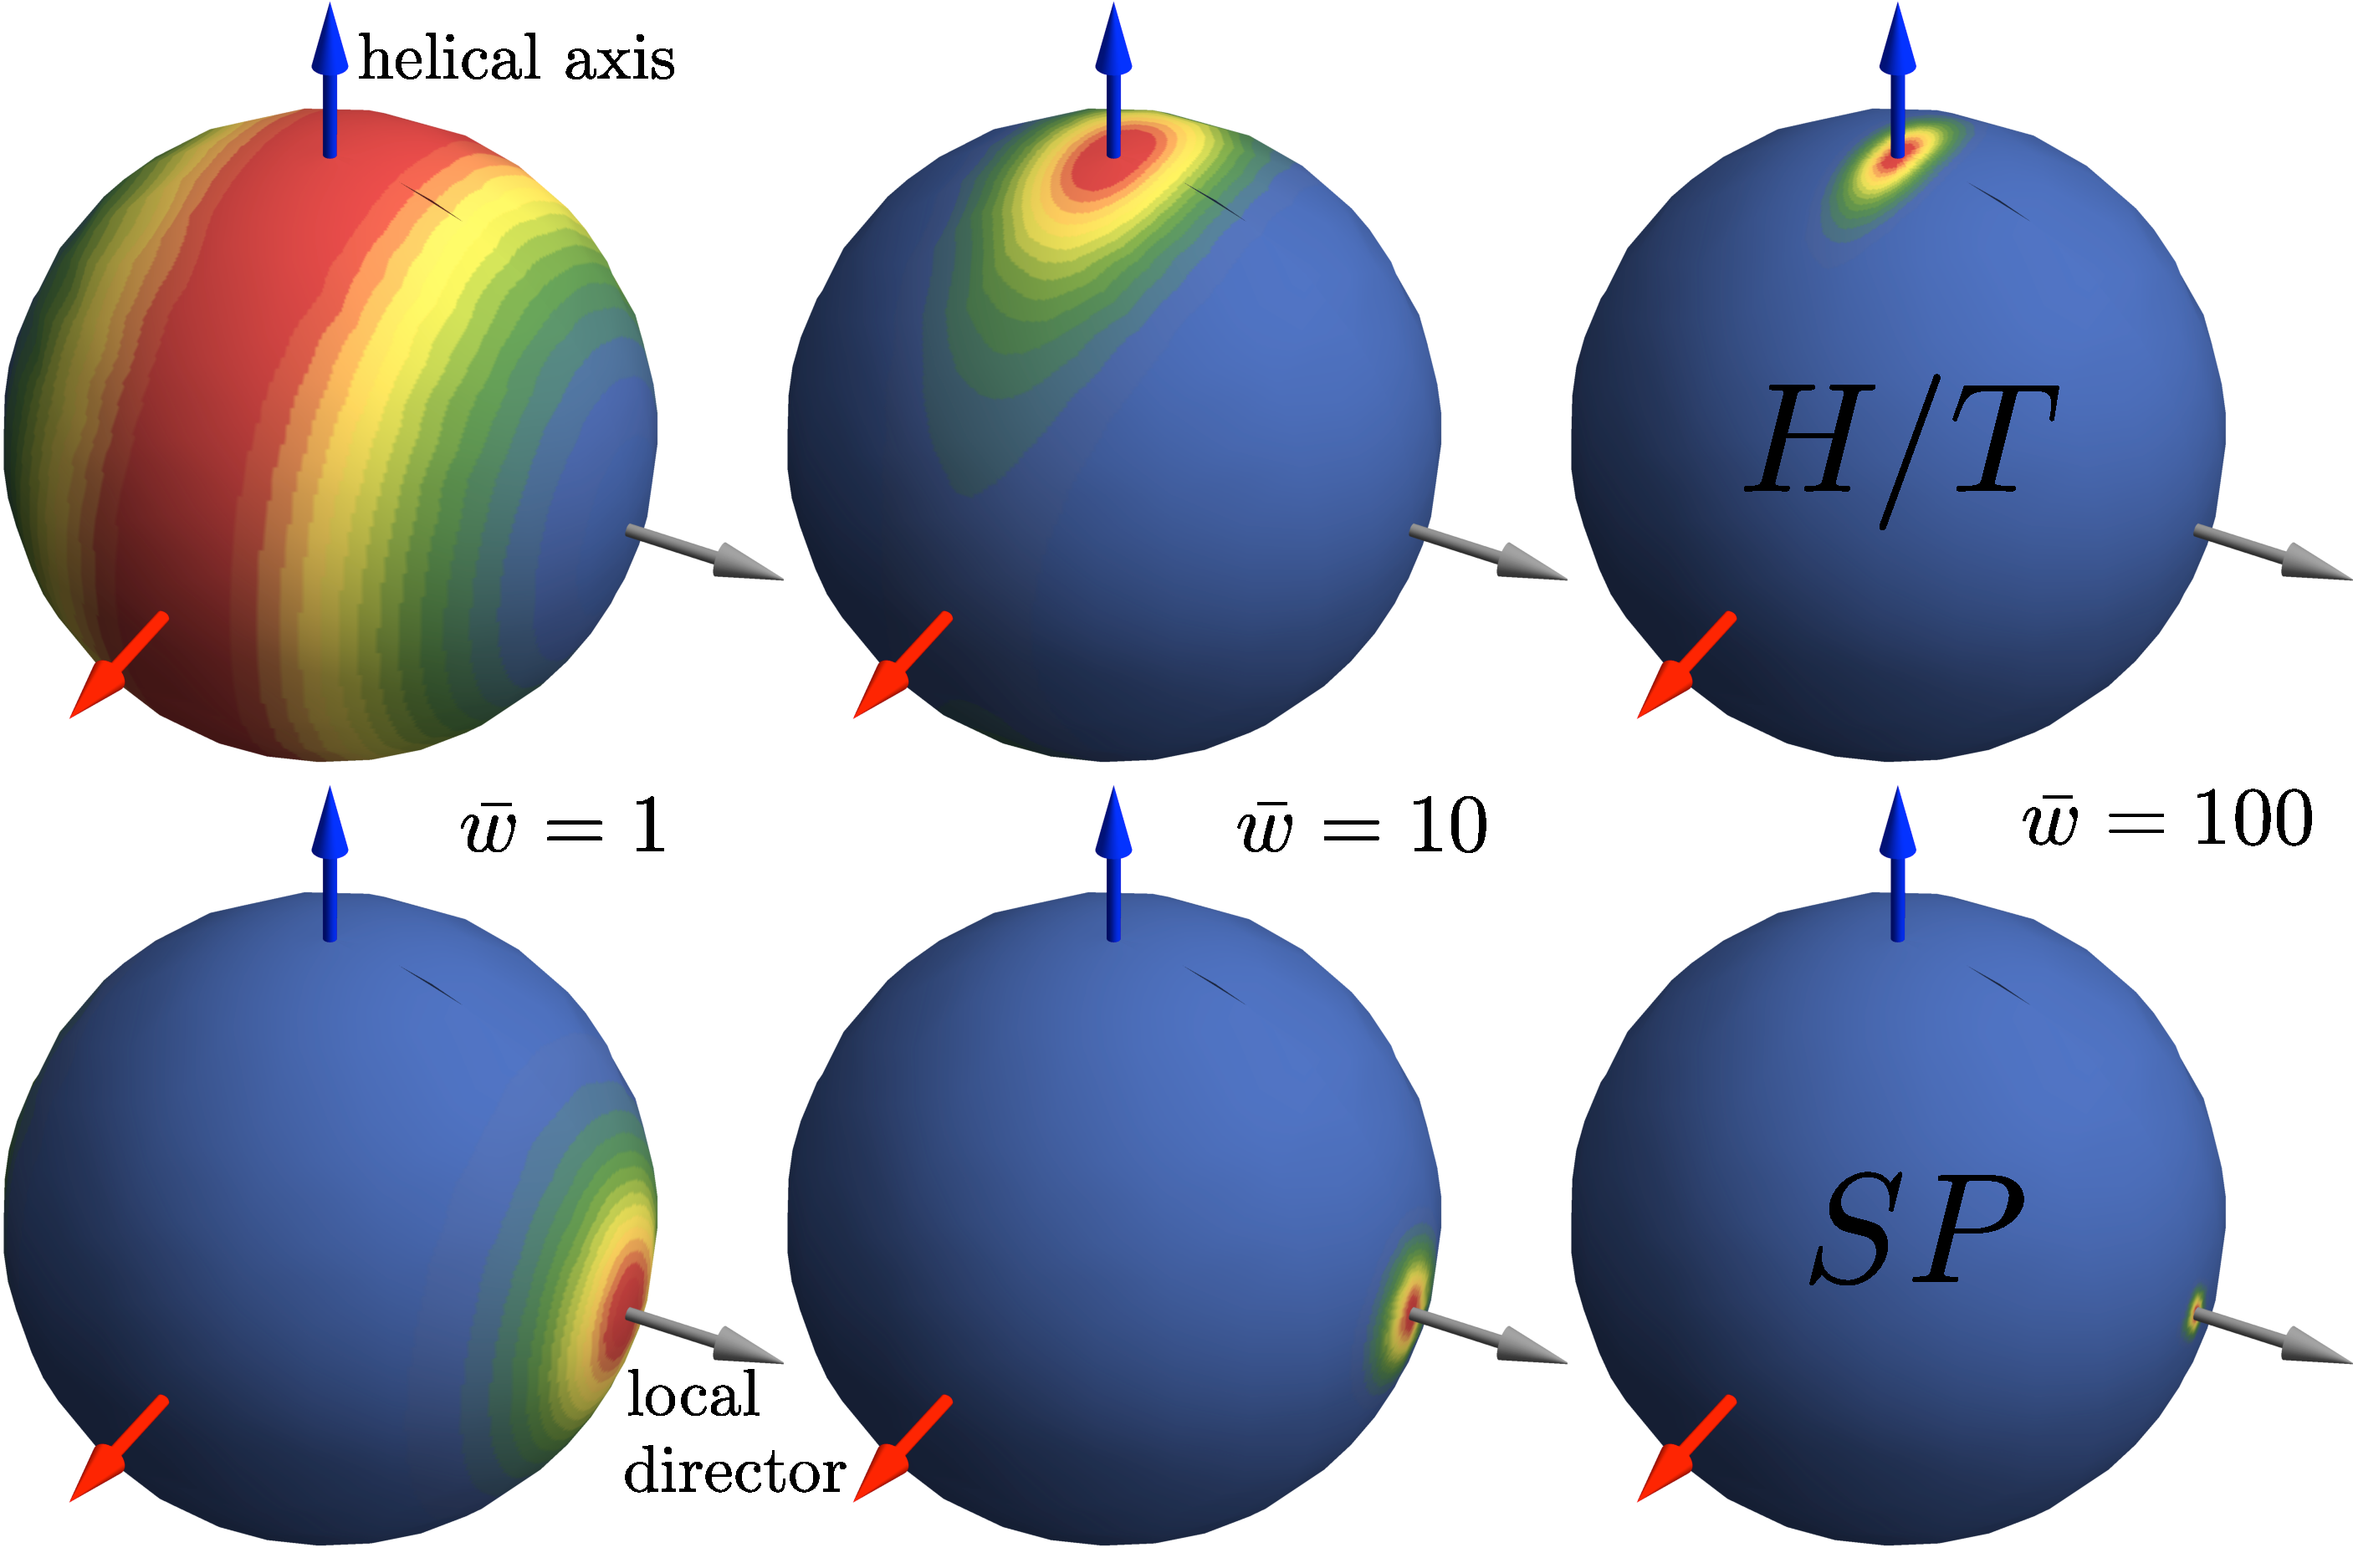
\includegraphics[width = 0.8\columnwidth]{figures/chapter-4/fcorr3}
	\caption{ Unit-sphere projections of the local orientational probability of rods immersed in a low molecular-weight cholesteric phase at different surface anchoring strengths $\bar{W} = \beta W_{0}LD$, in the presence of a low-correlated colloidal liquid crystal composed by particles of the same kind.  The rod concentration represented here is  $c= \rho L^{2} D = 3$ which corresponds to an isotropic bulk system in the absence of surface anchoring. For all distributions, the rod-length-to-pitch is $qL=1$.}
	\label{fcorr3}
\end{figure}

   \begin{figure}
	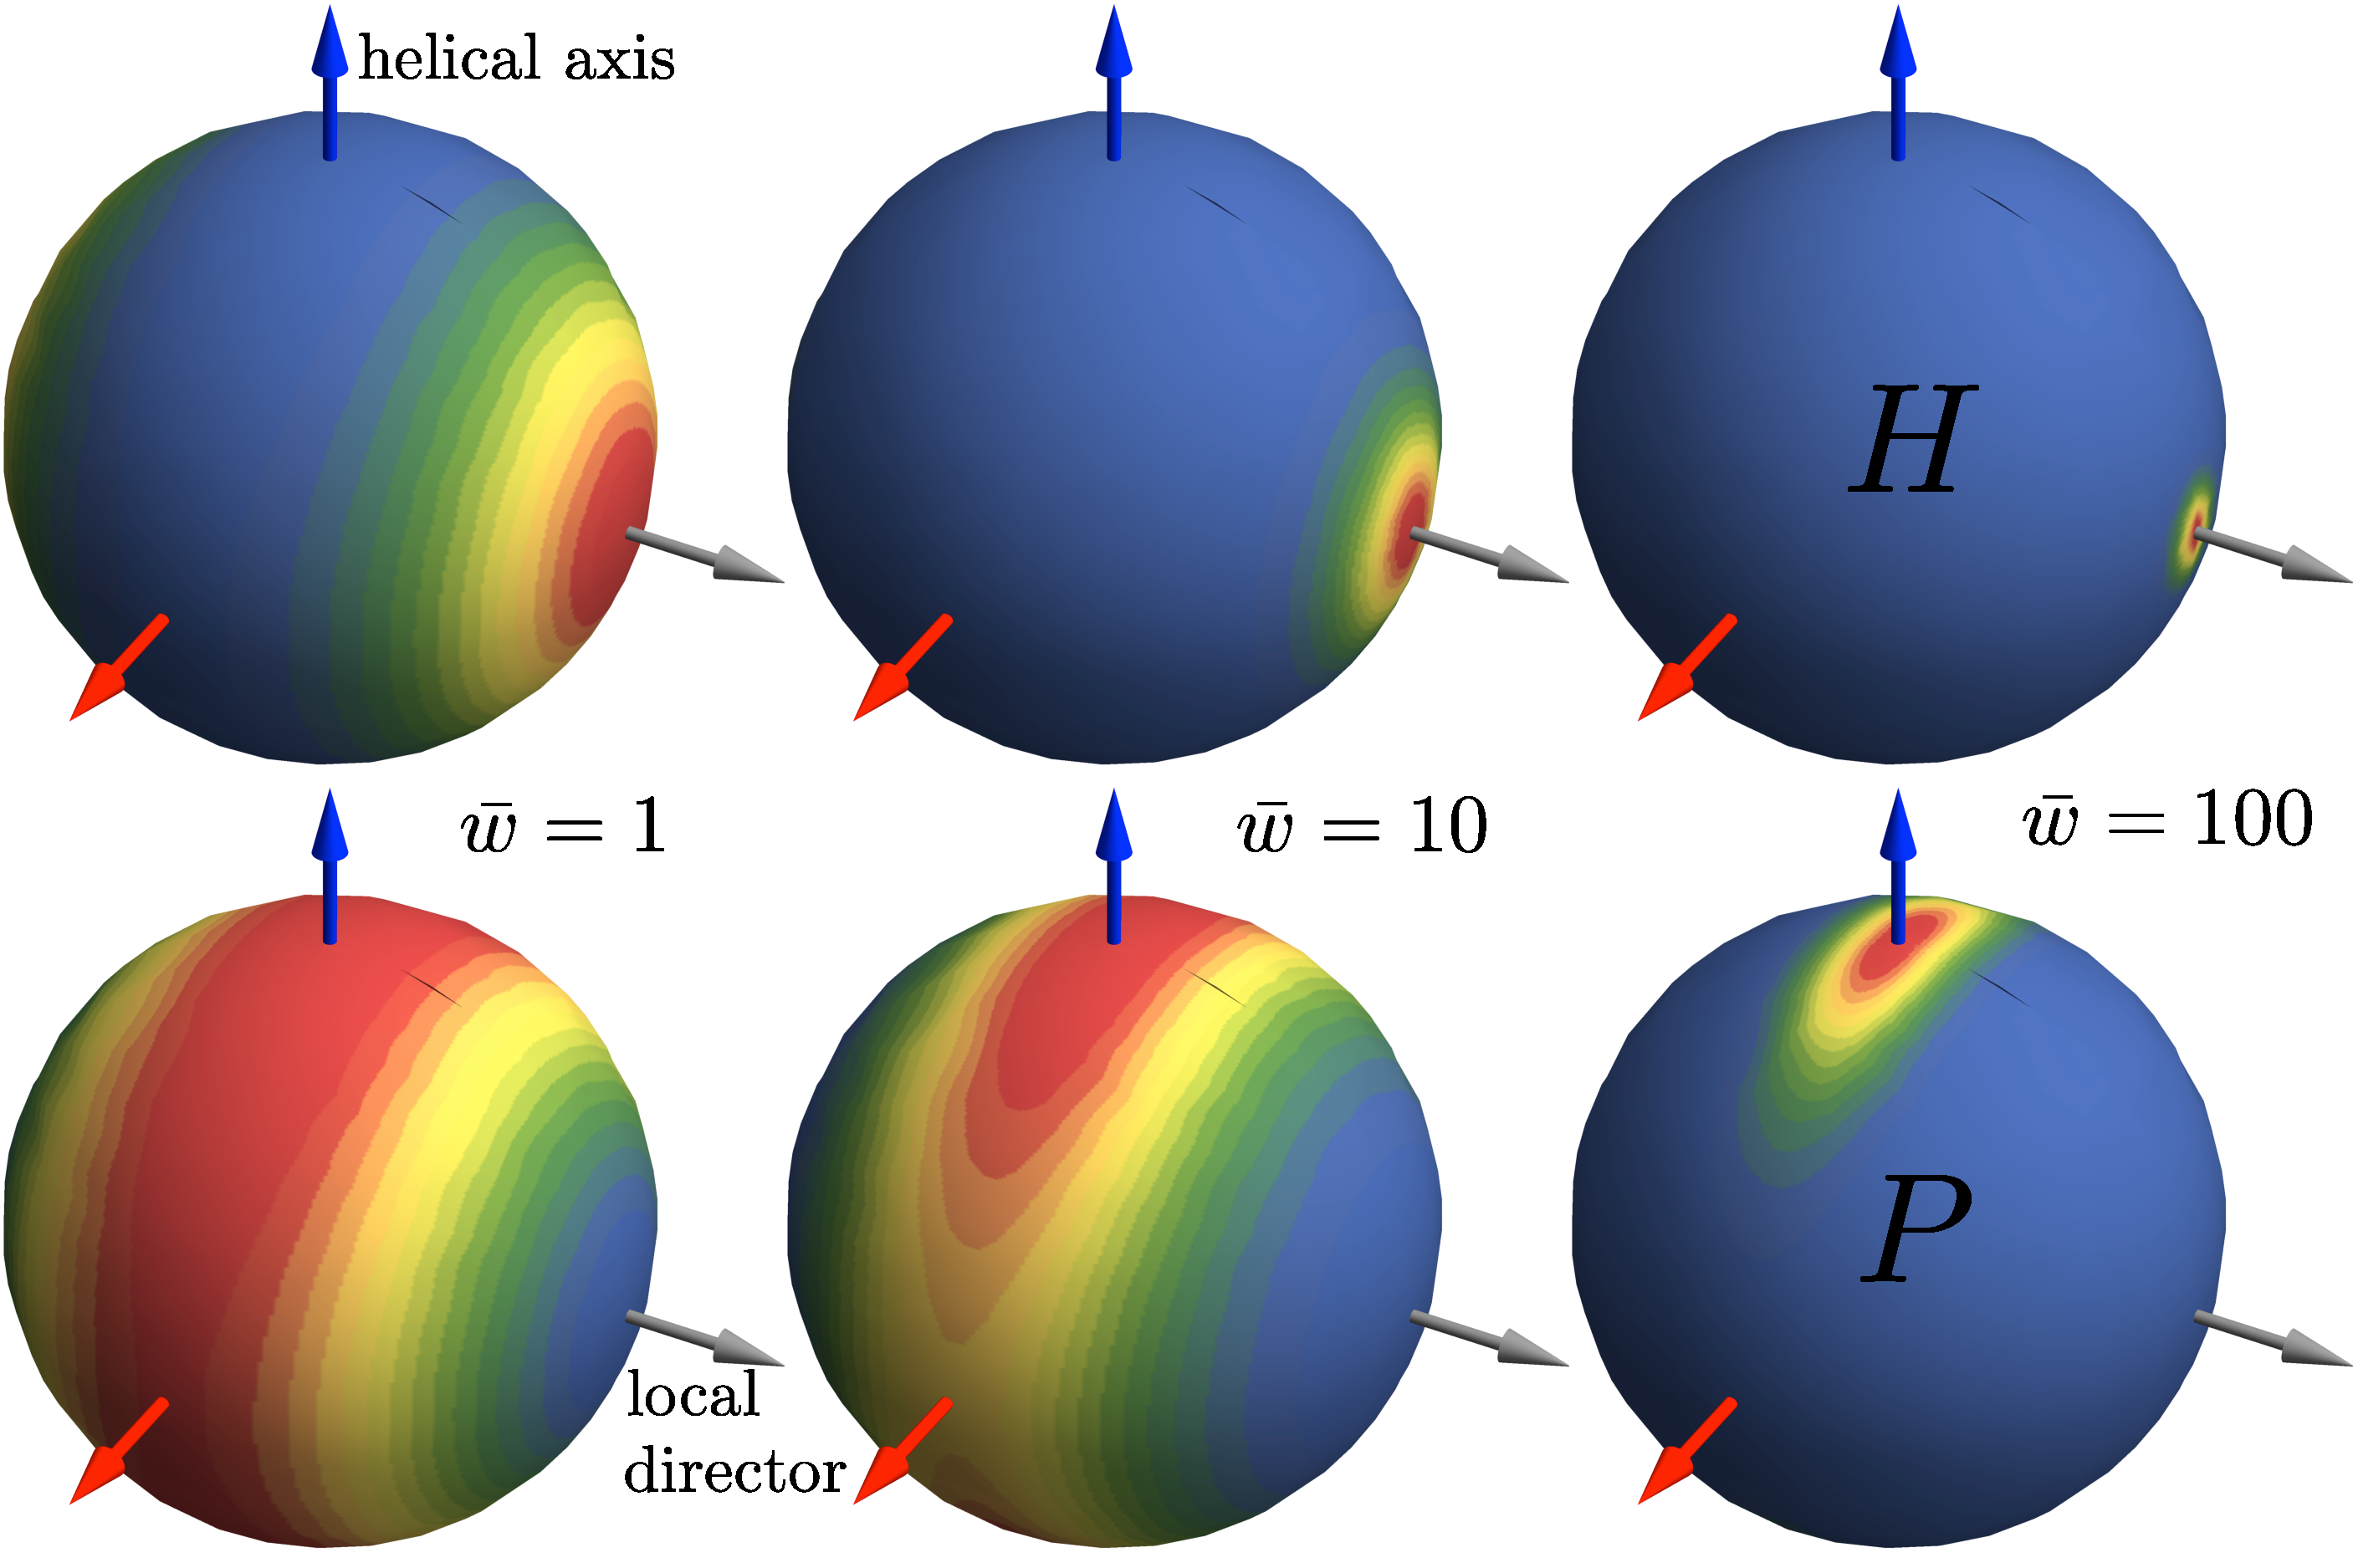
\includegraphics[width = 0.8\columnwidth]{figures/chapter-4/fcorrd3}
	\caption{ Unit-sphere projections of the local orientational probability of discs immersed in a low molecular-weight cholesteric phase at different surface anchoring strengths $\bar{W} = \beta W_{0}D^2$, in the presence of a low-correlated colloidal liquid crystal composed by particles of the same kind.  The disc concentration represented here is  $c= \rho D^3 = 3$ which corresponds to an isotropic bulk system in the absence of surface anchoring. For all distributions, the disc-size-to-pitch is $qD=1$.}
	\label{fcorrd3}
\end{figure}
Combining all free energy contributions and formally minimizing the Helmholtz free energy with respect to $f_{q}$ yields a Boltzmann distribution similar to \eq{fsingle}:
   \beq
  f_{q}( \bhu ) = \mathcal{N} \exp \left (- \beta  F_{s} (\bhu) - \rho \int d \bhu^{\prime} f_{q}( \bhu^{\prime} ) {\mathcal K}_{0}(\bhu, \bhu^{\prime})  \right )
  \label{fcollec}
  \eeq
  which reduces to the ideal gas probability \eq{fsingle} for vanishing rod density $\rho = 0$ as it should. The above condition needs to be solved iteratively for a given combination of dimensionless parameters pertaining to the rods (discs), namely the  cholesteric pitch $qL$ ($qD$), surface anchoring strength $\beta W_{0}LD$ ($\beta W_{0}D^{2}$) and colloid concentration $c = \rho L^{2}D$ ($\rho D^{3}$). Possible phase transitions can be probed from the osmotic pressure $\Pi \equiv \partial F/\partial V|_{N,T}$ and chemical potential $\mu \equiv \partial F /\partial N|_{V,T}$ which read:
  \begin{align}
  \beta \Pi  &= \rho + \frac{\rho^{2}}{2} \langle \langle {\mathcal K}_{0}(\bhu, \bhu^{\prime}) \rangle \rangle _{f_{q}} \nonumber \\
  \beta \mu &= \ln [\rho v_{0}] + \langle \ln [f_{q} (\bhu)] + \beta F_{s}(\bhu)\rangle_{f_{q}} + \rho \langle \langle {\mathcal K}_{0}(\bhu, \bhu^{\prime}) \rangle \rangle_{f_{q}}
  \end{align}
  The  brackets are shorthand for an orientational average $ \langle  \cdot  \rangle_{f_{q}} = \int d \bhu   f_{q}(\bhu )(\cdot)$ measured with respect to the local director.


   \section{Orthorhombic liquid-liquid phase separation}

In the absence of surface anchoring realignment ($\bar{W} = 0$) the colloids undergo a conventional isotropic-uniaxial nematic transition. This is the classic Onsager scenario where an isotropic (I) phase  ($c_{I} = 4.19$, $S_{I} =0$) coexists with a (uniaxial) nematic phase  ($c_{N} = 5.34$, $S_{N} =0.792$). For $\bar{W} >0$ the $O(3)$ symmetry of the isotropic phase and the uniaxial $D_{\infty h}$ symmetry of the nematic will both be broken in favour of a biaxial, orthorhombic symmetry ($D_{2h}$), and a coexistence between two orthorhombic phases with different overall colloidal concentrations is expected. Resolving the coexistence conditions by imposing equality of chemical potential $\mu$ and pressure $\Pi$ in both phases we may explore phase diagrams in the surface anchoring amplitude - colloid concentration ($\bar{W} - c$) plane. The results are shown in \fig{phdiag} and demonstrate that a phase coexistence between two orthorhombic nematic phases is indeed possible in the weak coupling regime ($\bar{W} <1$). A critical point beyond which no phase transition is possible is located at a surface anchoring energy equivalent to a few times the thermal energy.

   \begin{figure}
	\includegraphics[width = .9\columnwidth]{figures/chapter-4/diagrams_q0.335_horizontal}
	\caption{(a) $\bar{W} - c $ phase diagram for rods with homeotropic or tangential surface anchoring, $qL = 0.335$. (b) Corresponding uniaxial (solid line) and biaxial (dashed line) nematic order. A qualitatively equivalent scenario can be found for discs with planar surface anchoring.}
	\label{phdiag}
\end{figure}


   \begin{figure}
	\includegraphics[width = \columnwidth]{figures/chapter-4/ordervsc_rods}
	\caption{ Uniaxial $S$ and biaxial $\Delta$ order parameters measured along the cholesteric nematic direction $\bn_{m}$ as a function of the concentration $c = \rho L^{2}D$ ($\rho D^{3}$) for rods at low (dashed lines) and high (solid lines) surface anchoring strength ($\bar{W} = \beta W_{0}LD = 1$ and $\bar{W} = \beta W_{0}LD = 100$ respectively) and three different values of $qL$.}
	\label{w1o}
\end{figure}

   \begin{figure}
	\includegraphics[width = \columnwidth]{figures/chapter-4/ordervsc_discs}
	\caption{ Uniaxial $S$ and biaxial $\Delta$ order parameters measured along the cholesteric nematic direction $\bn_{m}$ as a function of the concentration $c = \rho L^{2}D$ ($\rho D^{3}$) for discs at experimentally typical surface anchoring strength ($\bar{W} = \beta W_{0}D^2 = 1$ and $\bar{W} = \beta W_{0}D^2 = 100$ respectively) and three different values of $qL$.  The concentration range evaluated in the discotic homeotropic case for $\bar{W} = \beta W_{0}D^2 = 1$ is more restricted due to  numerical difficulties.}
	\label{w100o}
\end{figure}




\section{Effect of colloid-induced elasticity}

At certain conditions such as strong surface-anchoring coupling and large colloid concentration $\rho$ and short cholesteric pitches the twist elastic resistance generated by the anisotropic colloid-colloid repulsions will prevent the colloidal director from keeping pace with the rotation of the cholesteric director. This  may give rise to hybrid systems in which the colloidal director locally deviates from the the cholesteric helix. Let us attempt to explore this scenario in more detail starting from the cholesteric director field \eq{ns} that we keep fixed in the laboratory frame. In doing so, we rely on three further basic assumptions; (i) the colloids remain uniformly distributed throughout the system and do not affect the cholesteric helix whose  pitch $q$ remains unaffected, (ii)  the colloids are perfectly aligned and exhibit negligible thermal fluctuations around their main orientation, and (iii) the colloidal director remains perpendicular to the helical axis $\bz$ but we allow the degree of local twist to be non-uniform along the $z$-direction. We then parameterize the colloidal director as follows:
\beq
\bn(z) = \bx \cos \phi(z)   + \by \sin \phi(z)
\label{npara}
\eeq
 in terms of a local twist angle $\phi(z)$. Since the system is apolar, the director $\bn$ is equivalent to $-\bn$ so that $\phi(z)$ is equivalent to $\phi(z)  + \pi$.  For the cases discussed thus far, the colloidal director is simply co-helical with the cholesteric so that $\phi(z) =qz$ (mod $\pi )$.

 \subsection{Rods}

 Let us focus first on the case of rods. The fraction of rods aligned along the helical axis $\bz$ (as observed in \fig{fcorr3}) may be disregarded as they contribute very little to the twist elastic resistance imparted by the colloids. Since we assume that the rods are perfectly aligned along the above director we write the rod contour $\bfr_{{\mathcal S}}(t) = \bfr_{0} +  \frac{L}{2}t\bn(z)$ and applying this in the Rapini-Papoular expression \eq{usurf} along with the above parameterization we find:
\beq
F_{s}[\phi(z)]  = - \frac{1}{8} W_{0} LD \begin{cases}
       2 \pi \sin^{2}[\phi(z) -qz ] &  \textrm{H/T} \\
         4 \pi \cos^{2}[ \phi(z) - qz ]  &  \textrm{SP}
   \end{cases}
      \label{plahoms}
\eeq

In the absence of twist elastic effects the surface anchoring energy is indeed minimized along a uniform twist profile $\phi(z) = qz + \phi_{0} $ with phase shifts $\phi_{0} = \pi/2$ (H/T) and $\phi_{0} = 0$ (SP) as evident from the result in \fig{fcorr3} and \fig{fcorrd3}.


The (continuum) free energy per unit area reflects a competition between the surface anchoring energy, and a restoring (twist) elastic energy:
\begin{align}
\frac{F}{A} &= \int d z \left \{ \rho F_{s}[\phi(z)]  + \frac{K_{2}}{2} (\bn(z) \cdot \partial \times \bn(z) )^{2} \right \}
\end{align}
with $K_{2}$ the twist elastic modulus of a colloidal nematic system.
Removing the trivial phase angle by rescaling $\phi(z) \rightarrow \phi(z) - \phi_{0}$ and some further basic manipulation we obtain a universal expression for both anchoring scenarios:
\beq
\frac{F}{A} = \int d z \left \{ -\sigma \cos^{2}[\phi(z)-qz] + \frac{K_{2}}{2} (\partial \phi(z)  )^{2} \right \}
\label{freedens}
\eeq
in terms of surface anchoring energy density $\sigma_{\ds \rm HT} = \tfrac{\pi}{4} \rho W_{0}LD$ and $\sigma_{\ds \rm SP} = 2 \sigma_{\ds \rm HT}$ for the SP case. The corresponding Euler-Lagrange equations reads:
\begin{align}
 K_{2}\phi^{\prime \prime}(z) - \sigma \sin[2 ( \phi(z)- qz)]&=0
 \label{nlde}
 \end{align}
subject to the boundary conditions $\phi(0) = 0$ and $\phi^{\prime}(0) = 0$, i.e., the colloids are kept non-chiral. The effect of chirality will be considered in a subsequent paragraph.
It is convenient to introduce a non-linear twist angle $\varepsilon(z) = \phi(z) - qz$ which measures the local deviation of the colloidal director from the cholesteric one. Both anchoring situations can then be described by a sine-Gordon equation:
\beq
 \xi^{2} \varepsilon^{\prime \prime}(z) = \sin[2\varepsilon(z) ]
\label{diffeps}
\eeq
It features the following length scale:
\beq
\xi = \sqrt{\frac{K_{2}}{\sigma}}
\eeq
The  solution under is non-analytical and can be written in terms of (inverse) elliptic functions:
\beq
\phi(z) = qz -\textrm{am} (qz, -2/(q\xi)^{2})
\label{jaf}
\eeq
with $\textrm{am}(x,k)$ denoting the Jacobi amplitude function which has the known limit $ \textrm{am}(x,0) = x$. From this we conclude that an untwisted director profile $\phi(z) = 0$ is found at infinite elasticity $q\xi \rightarrow \infty$, as should be the case. At large but finite $q\xi$ the colloidal helix unwinds with respect to the cholesteric and adopts an (average) pitch $q_{c} <q$, leading to a bi-helical hybrid system. This scenario is depicted in \fig{unwind}. Interestingly, at $q\xi >1$ the colloidal helix not only unwinds, it also adopts a handedness that is opposite that of the cholesteric helix.  Associated with the unwound colloidal director are periodic ``breathing" fluctuations whose amplitude and period are shown in \fig{fluc}.  These fluctuation are easily fitted to a periodic profile so that (for $q \xi >1$):
\beq
\phi(z) -q_{c}z \approx   \delta \phi e^{  i q_{b} z }
\label{nlinrip}
\eeq
in terms of an amplitude $\delta \phi$ and periodicity $q_{b}$. The amplitude slowly decays as $q \xi \rightarrow \infty $ while the breathing periodicity attains a constant value $q_{b}/q \rightarrow 2$.


   \begin{figure*}
	\includegraphics[width =  \columnwidth]{figures/chapter-4/bihelical}
	\caption{ (a) Twist angle $\phi(z)$ of the colloidal director along the helical direction for different strengths of the twist elasticity of the colloids. At weak twist elasticity  ($q \xi <1$) the colloidal director remains co-helical with the cholesteric helix.  At $q \xi >1$ unwinding of the colloidal helix occurs with  ``breathing" instabilities.   (b) Evolution of the pitch $q_{c}$ of the colloidal helix with respect to the cholesteric pitch $q$. Note that in the bi-helical regime the cholesteric and colloidal helices have opposite handedness. The colloidal helix is shown in red, the molecular one in blue.   Colored dots indicate the  state-point corresponding to the breathing profiles in (a). }
	\label{unwind}
\end{figure*}


 \begin{figure}
	\includegraphics[width = .6\columnwidth]{figures/chapter-4/fluctuations}
	\caption{ Amplitude $\delta \phi$ and periodicity $q_{b}$ of the ``breathing" instabilities encountered in the bi-helical state in \fig{unwind}b as a function of the twist elastic strength $q \xi$. }
	\label{fluc}
\end{figure}

Another common solution that is associated with the sine-Gordon equation is the soliton. Taking the boundary conditions $\varepsilon^{\prime}(\pm \infty) = 0$ and $\varepsilon(\infty) - \varepsilon(-\infty)  = \pi$. The solution for the single soliton can be obtained in analytical form  \cite{kamien2001order}:
\beq
\phi(z) =  qz \pm \frac{\pi}{2} \pm 2 \arctan \left [ \tanh \left ( \frac{z - z_{0}}{R_{s}} \right ) \right ]
\eeq
where $ R_{s} = 2^{1/2} \xi$ defines the soliton width and $z_{0}$ the arbitrary position of its centre along the cholesteric helix. The $-$ solution refers to an anti-soliton. In achiral liquid crystals such as our colloidal subsystem, the (anti-)solitons are unstable with respect to the uniform background (i.e. the co-helical state). The dimensionless free energy difference between the soliton and the co-helical state is  $\tfrac{\Delta Fq}{ A \sigma} = q \xi (2^{3/2} + \pi q\xi)$. However, once they are formed the solitons are metastable and cannot simply relax to the co-helical state without locally destroying nematic order.

From the scaling expression \eq{k2odijk} for the twist elastic constant of rods proposed in the Appendix we find that the soliton width $\sim \xi$ is independent of rod concentration. However, the solitons would be unrealistically small as $\xi $ turns out to be of the same scale as the width of the individual rods, namely  $\xi \sim 70 nm$ for long rods ($L \sim 3 \mu m$ and $D \sim 30 nm$ and $W_{0} = 10^{-5} J/m^{2}$).


\subsection{Effect of rod chirality}

It is well known that conventional (non-hybrid) chiral liquid crystal subject to a uniform electromagnetic field perpendicular to the helical axis may form stable solitons provided that the nematogens are sufficiently chiral \cite{lam2012solitons,ackerman2014two,wu2022hopfions}.  In fact, our rods must have some intrinsic chirality in view of the decoration of helical disclinations imparted by the cholesteric environment, as demonstrated in the previous chapter. The effect of chirality is easily accounted for by an additional free energy \cite{gennes-prost}:
\begin{align}
\frac{F_{\rm chiral}}{A} &= K_{t} \int d z  (\bn(z) \cdot \partial \times \bn(z) )=  K_{t} \int d z (\partial \phi(z) )
\end{align}
with $K_{t}$ denoting the strength of the chiral interactions between the rods. It is customary to identify $K_{t} =q_{r} K_{2}$ where $q_{r}$ would be the pitch of a chiral nematic formed by the rods {\em alone}. In general, $q_{r}$ differs from the pitch $q$ of the cholesteric helix $q$ although a subtle coupling between the two is expected. We stress that $q_{r}$  is a purely hypothetical variable since the rods would not be chiral in the absence of surface anchoring effects imparted by the cholesteric solvent.
Since the chiral contribution is linear in the gradient of $\phi$, the Euler-Lagrange equation \eq{nlde} associated with the total free energy remains unchanged. The boundary conditions now read $\phi(0) = 0$ and $\phi^{\prime}(0) = q_{r}$. If we assume the handedness of the rods to be the same as that of the cholesteric environment, then the main effect of colloid chirality is that the co- to bi-helical transition shifts towards larger $q \xi$. This is a natural consequence of the fact that chirality favors the twisted co-helical state over the (partially) untwisted bi-helical one. Of course, the reverse effect occurs if the rods adopt a handedness that is opposite to that of the cholesteric state ($q_{r} <0$). Then, the transition to the bi-helical state in \fig{unwind}b systematically shifts to smaller $q\xi$ upon increasing the chiral strength $|q_{r}|$.


The free energy between the soliton and the  co-helical state now reads $ \tfrac{\Delta Fq}{ A \sigma} = q \xi [ 2^{3/2}+  \pi q \xi (1-\tfrac{q_{r}}{q})]$. This means that solitons may eventually become stable within the co-helical regime if $\tfrac{q_{r}}{q} > 1 + \tfrac{2^{3/2}}{\pi q \xi}$ which implies that the rods must be very strongly chiral indeed. However, the soliton width is not affected by chirality and remains of the order of the colloid thickness which means that the solitons remain a purely hypothetical scenario, at least within our simple coarse-grained model.

\subsection{Discs}

The case of discs proceeds in an analogous way.  If we assume the same set of basic approximations to hold for the colloidal discs as well, we may start with computing the surface anchoring free energy which takes a simple form  (ignoring irrelevant constants):
\beq
F_{s}[\phi(z)]  =   \begin{cases}
       -\sigma_{\rm \ds H} \cos^{2}[\phi(z) -qz ] &  \textrm{H} \\
        -\sigma_{\rm \ds P} \sin^{2}[ \phi(z) - qz ]  &  \textrm{P}
   \end{cases}
      \label{plahomsdisc}
\eeq
with $\sigma_{\rm \ds H} = \frac{\pi}{4}\rho W_{0}D^{2}\tfrac{J_{1}(qD)}{qD}$ and $\sigma_{\rm \ds P}= \tfrac{1}{2} \sigma_{\rm \ds H}$ describing the two basic anchoring symmetries we consider. Comparing with \fig{fd} we immediately identify the optimal profile $\phi(z) = qz + \phi_{0}$ with $\phi = 0$ (H) and $\phi_{0} = \tfrac{\pi}{2}$ (P) at least for weak to moderate cholesteric pitch $qD < 2$.   Clearly, since the surface anchoring energy has the same basic form  as those previously discussed in \eq{plahoms} for  rods, the director profiles are identical too, provided the  lengthscale $\xi =\sqrt{K_{2}/|\sigma|}$ is taken to be the one appropriate for discs. Using the scaling expression from the Appendix, we find:
\beq
\xi \sim 0.87 c  \sqrt{  \frac{|q|D}{J_{1}(|q|D)}} \sqrt{\frac{k_{B}T}{W_{0}}}
\eeq
which yields about $\xi \approx 80 nm $ for $D = 2 \mu m$ sized discs studied experimentally at a concentration $c = \rho D^{3} =3$, $W_{0} = 10^{-5} J/m^{2}$ and a cholesteric pitch length of $30 \mu m$ corresponding to $qD \approx 0.6$.

For certain values of $qD$ the surface anchoring amplitude $\sigma $may become negative ($\sigma< 0$). In those cases, the phase angles associated with the two anchoring scenarios are simply swapped so that  $\phi = \tfrac{\pi}{2}$ (P) and $\phi_{0} = 0$ (P). By rescaling $\phi(z) \rightarrow \phi(z) - \phi_{0}$ we obtain the  same Euler-Lagrange equation \eq{nlde} with $\sigma \rightarrow | \sigma |$.


\section{Conclusions and outlook}

In this chapter we have theoretically addressed the implications of finite colloid concentration in self-organization of hybrid colloidal-molecular liquid crystals. While at low colloid content the orientation of each colloid is mainly driven my single-particle effect related to surface anchoring and possible surface defects, the phenomenology becomes richer and exciting when colloid-colloid interactions are taken into account. We argue that steric combined with weakly aligning surface anchioring forces may drive liquid-liquid phase separation between two orthorhombic fluid, each with a different colloid concentration and orientational order parameters. In the strong coupling regime, when surface-anchoring-mediated  particle realignement is strong, the colloids impart non-negligible twist elasticity that may stabilize a variety of different bi-helical hybrid LCs in which both molecular and colloidal self-organize along distinctly different helical mesostructures. We also predict the typical colloidal concentration needed to stabilize these structures in experiment. 

At elevated colloid concentration additional interactions could becomes more prominent, for instance those imparted by surface defects and long-range electrostatic forces owing to surface charges residing on the colloids, which will have an impact on the elastic properties generated by the colloids. In fact, one could naively argue  that these could give rise to a significant stiffening of the elastic moduli of the colloidal subcomponent which could lead to a stabilization of bi-helical structures at much lower colloid concentrations than anticipated here.   Clearly, any further quantitative prediction requires a considerable refinement of our analysis beyond the simple steric model considered here.  






%A general solution of \eq{nldereno} under the boundary condition $\varepsilon(0)=0$ can be expressed in terms of the Jacobi amplitude (am) function:
%\beq
%\varepsilon(z) = \textrm{am} \left (qz c_{1}, \frac{2}{- c_{1}^{2} (q\xi)^{2}} \right )
%\eeq
%with $c_{1} > 0$ some unknown constant that needs to be determined from the second boundary condition.







%yields the basic solution $\varepsilon(z) = \varepsilon_{-} \exp(-2^{1/2} z/\xi)+ \varepsilon_{+} \exp(2^{1/2} z/\xi)$. Imposing the boundary condition  $\varepsilon(0) =0$ we find:
%\beq
%\varepsilon(z) = 2\varepsilon_{0} \sinh ( 2^{1/2} z/\xi )
%\eeq
%Since the hyperbolic sine diverges for large $|z|$ the only way to render the solution consistent with $|| \varepsilon ||$ is by setting $\varepsilon_{0} =0$ which means there are no solutions up to linear order in $\varepsilon$.

%Reduction of order leads to
%\beq
%( \varepsilon^{\prime} (z) )^{2} + (q\xi)^{-2} \cos [2 \varepsilon(z)] = C_{1}
%\eeq

\begin{subappendices}
\section{Twist elastic resistance of thin hard needles and discs}

For   hard rods  a tractable analytical expression for the $z-$resolved excluded area is available in the needle limit $L/D \rightarrow \infty$ \cite{poniewierski1988nematic,shundyak2001isotropic}:
\begin{align}
 & {\mathcal A}(|  \Delta z | , \bhu, \bhu^{\prime} ) = -\int d  \Delta \bfr_{\perp} \Phi(|\Delta \bfr |, \bhu, \bhu^{\prime} ) \nonumber \\
 & = 2 L^{2} D |\sin \gamma | \begin{cases}
 0 & |\Delta z| > A+ B \\
 \frac{A + B - |\Delta  z |)}{4 AB } & A - B \leq |\Delta z| \leq A+ B  \\
 \frac{1}{2A} & |\Delta z| < A - B
 \end{cases}
 \label{aexcl}
\end{align}
with $A= \frac{L}{2} | \text{max} ( u_z , u^{\prime}_{z}  ) |$ and $B= \frac{L}{2} | \text{min} (u_{z} , u^{\prime}_{z} ) |$.  We can make headway by realizing that  a rotation of the reference director  only affects the azimuthal angle $\varphi$. More specifically we  have
 ${\mathcal R}(q \Delta z) | \sin \gamma | = \sqrt{1 - (\cos \theta \cos \theta^{\prime}  - \sin \theta \sin \theta^{\prime} \cos (\Delta \varphi - q\Delta z) )^{2}} $
with $\Delta \varphi = \varphi - \varphi^{\prime}$.  Performing the integration over $\Delta z$ we can cast the kernel as a Taylor series in terms of even powers of the colloidal pitch $qL$:
\beq
{\mathcal K}_{q} (\bhu, \bhu^{\prime}) = 2 L^{2} D \sum_{n=0}^{\infty} \frac{(qL)^{2n}}{2n!} a_{2n} (\bhu, \bhu^{\prime})
\eeq
 Note that odd powers in $q$ must vanish since the rods are considered to be achiral. We note that  the immersed rods induce weak distortions of the solvent director which are known to adopt a helical signature that could render the rod-rod interaction chiral.  The angle-dependent factor reads in explicit form:
\begin{align}
a_{2n} (\bhu, \bhu^{\prime}) &=  \frac{(\frac{1}{2}u_{z}+\frac{1}{2}u^{\prime}_{z})^{2n +2} - ( \frac{1}{2}u_{z} - \frac{1}{2}u_{z}^{\prime})^{2n+2}}{ u_{z} u_{z}^{\prime} (2n+1)(n+1)} \nonumber \\
& \times \frac{\partial ^{(2n)} | \sin \gamma |_{q=0}}{\partial \Delta \varphi ^{(2n)}}
\end{align}
and it is easily verified that $a_{0} = | \sin \gamma |$ as required. It is insightful to express the  excess free energy per unit volume in the following way:
\beq
\frac{F_{ex}}{V} = k_{B}T \frac{\rho^{2}}{2} \langle \langle {\mathcal K}_{0}(\bhua, \bhub) \rangle \rangle_{f_{q}} +  \sum_{n=1}^{\infty} \frac{q^{2n}}{2n!} K_{2}^{(2n)}
\label{felast}
\eeq
 The quantities $K_{2}^{(2n)}$ could be interpreted as {\em generalized} twist elastic constants defined as:
\beq
K_{2}^{(2n)} = k_{B}T \rho^{2} L^{2n+2}D \langle \langle a_{2n}(\bhua, \bhub) \rangle \rangle_{f_{q}}
\eeq
for most conventional cholesteric phases the director twist is weak on the scale of the rod ($qL <1$) and the expansion may be truncated after the second term. Furthermore, the  orientation distribution is   unaffected by any director twist so that $f_{q}$ can be approximated by the orientation distribution $f_{0}$ of a non-chiral uniaxial nematic phase. The  quantity $K_{2}^{(2)}$ is then identified as the conventional twist elastic constant for which the microscopic definition reads:
\beq
K_{2}  =K_{2}^{(2)}=  k_{B}T \rho^{2} L^{4}D \langle \langle a_{2}(\bhu, \bhu^{\prime}) \rangle \rangle_{f_{0}}
\eeq
For conventional uniaxial nematic order scaling results exist that relate  $K_{2}$ to the total  rod concentration. Using Gaussian theory Odijk \cite{odijkelastic} found that for asymptotically strong nematic alignment:
\begin{align}
\beta K_{2}D \sim \frac{7}{96} c
\label{k2odijk}
\end{align}
For infinitely thin hard discs a much steeper increase with colloid concentration was found \cite{wensink2018}:
\beq
\beta K_{2}D  \sim 0.606 c^{3}
\eeq
which suggests that lyotropic discotic nematic phases are far more difficult to twist than their rod-based counterparts at equivalent particle concentration (note that $c \gg1$ for most stable nematics).

\end{subappendices}


\clearpage % Cholesterics: single colloid

\chapter{ Twisted membranes versus ribbons in colloidal rods stabilized by polymer depletion}
\chaptermark{Tactoid morphology}



\begin{abstract}

At the mesoscopic level, rigid rodlike colloids with chiral features such as {\rm fd} virus rods mixed with non-adsorbing polymer form a variety of different liquiod crystalline droplets with varying shape and internal twisted structure. Inspired by recent experiment work on the droplet morphology of these rod-polymer mixtures, we use extensive Monte Carlo simulations supplemented with theory to explore two prominent droplet shapes, namely the twisted membrane and the ribbon. In experiment, the elongated ribbon structure is found to dominate at elevated chiral strength. In our simulations, however, we demonstrate that upon increasing chirality the membranes tend to transition into multi-domain structures consisting of multiple twisted near-circular units separated by $\pi$-walls, while the transition into twisted ribbons appears impeded for reasons unknown. We supplement our simulations with simple microscopic theoretical descriptions for both droplet morphologies which enable us to predict the evolution of the twist angle across the membranes.  We finish by  briefly discussing the role of planar confinement on the droplet morphology in relation to recent experimental work on {\em fd}-polymer mixtures.

\end{abstract}



\section{Introduction}




Rodlike colloidal particles are capable of assembling into a variety of liquid crystalline mesostructures whose bulk properties depend primarily on the topology of the director field indicating the average direction of rod alignment \cite{dogic-fraden_fil,Ikkala2407}.
In general,  site-specific attractive forces between non-spherical nanoparticles may affect the self-assembly properties  and lead to a wealth of different superstructures \cite{Wang358} such as twisted ribbons of semi-conducting rods \cite{Srivastava1355} or platelets \cite{Janae1701483}.
Mixing rodlike colloids with non-adsorbing polymers or other small depletant particles induces a short-ranged attractive  (`sticky') effective potential between the rods that can be exploited to control the self-assemby morphology \cite{Baranov2010,Sharma2014}. 
 


 The size and concentration of the added polymer can be exploited to  tune the morphology and internal structure of the droplets. Tactoids with nematic-type order have been observed experimentally in mixtures of rods and big depletants (typically bigger than the diameter of the colloidal rods), as well as smectic-like single layer droplets, named colloidal membranes, when significantly increasing polymer concentration. The morphology of these membranes is further controlled by strong electrostatic and chiral twist interactions between the individual rods. Though these interactions are not well understood yet, it has been empirically observed that, in close contact with one another, {\em fd} rods tend to twist preferentially clockwise, instead of arrange following a global nematic direction. When both depletion effect and chirality are strong, twisted colloidal membranes tend to destabilize to give way to twisted ribbons. The additional effect of intrinsic particle chirality
strongly impinges  onto the self-assembled mesostructure and drives a vast range of different twisted or chiral structures ranging from smectic membranes to chiral ribbons  \cite{Gibaud2014} and hexagonal nanocrystals displaying screw-dislocations \cite{grelet1}. These twisted structures have been observed experimentally, but reproducing the various mesophases with distincltly different twisted morphologies in computer simulation has been elusive so far.  Modelling efforts have focussed almost exclusively on twisted membranes \cite{kang_sm2016,wensink2018elastic,kuhnhold2022colloidal} or conventional LC tactoids exhibiting full three-dimensional fluidity \cite{prinsen2003shape,prinsen2004parity,kuhnhold2022structure}. Resembling the local fluid structure of a smectic monolayer these membranes  provide a convenient platform  to address the typical length scale, called penetration length, over which twist is expelled from the edges of a colloidal smectic phase \cite{barry2009direct}. The concept of twist-expulsion was introduced by De Gennes in the 1970s who established an analogy between the smectic A phase and superconductors. It follows that smectic layers expel twist deformations in the same way that superconductors expel magnetic field \cite{gennes-prost}.



In a recent study Kuhnhold et al. \cite{kuhnhold2022colloidal} have reported an extensive simulation study of the properties of twisted membranes comparing numerical results with theoretical predictions. In order to facilitate the membranes were keeping the rod centres-of-mass were constrained to reside on the smectic plane, thereby suppressing out-of-plane fluctuations. While the constraint should be reasonable harmless for the flat membranes it does preclude the system from engaging in further morphological transitions such as the formation of ribbons and other filamentous structures observed in experiment \cite{Gibaud2014} and conjectured in continuum theory \cite{kaplan2010theory,kang_sm2016}. The aim of this study is re-address the stability and microstructure of membranes by exploring the full degrees of freedom of the rods. To describe rod-polymer mixtures we use large-scale Monte Carlo simulations of the well-known Asukara-Oosawa model comprising hard-spherocylinders mixed with penetrable hard spheres. The latter represent small polymers that are excluded from the sphercocylinder surface but do not feel each other (ideal polymer). This model is at the core of a range of free-volume theories that address the bulk thermodynamic properties and phase behavior of colloidal particles of  various shapes mixed with non-adsorbing polymers \cite{LekkerkerkerTuinier2011}. The spherocylinder interactions are rendered chiral by means of a simple pseudo-scalar potential that finds widespread sue in computer simulation. Thus, we have a model system where chiral twist competes with short-ranged attractive depletion interactions and surface tension in driving mesoscopic liquid crystalline droplets of various internal structure and shape.  In our simulations based on the semi-grand ensemble we fix the polymer chemical potential in the hypothetical reservoir containing polymeric spheres at a high enough value to prevent the droplets from dissolving and systematically vary the chiral interactions between the rods.

Further complexity can be achieved by the presence of strong geometric confinement.  In this study we will consider a slab geometry with width comparable to the rod length. The confinement is expected to generate tactoids with a strongly non-uniform rod density whose morphology is further controlled by a surface tension that strongly depends on the average rod orientation with respect to the surface normal. In fact, the presence of the wall imparts a wall-liquid surface tension which is likely to be different from the liquid-gas surface tension which would dominate in the bulk case. We demonstrate that the presence of walls lead to .....



\section{Model and simulations}

We consider a system of $N$ rigid spherocylinders of length $L$, thickness $D$ and aspect ratio \red{$L/D = 10$ or $20$}. The spherocylinders are a simplified representation of {\em fd} rods that are much thinner ($L/D > 100$) and carry a small degree of backbone flexibility with persistence length $\ell_{p} \gg L$. Since the large particle aspect ratio in combination with backbone flexibility poses considerable limitations on the numerical efficiency of our simulations  we  only consider rigid rods with a relatively short length assuming that the key features of the mesoscopic structures evaluated in this work do not  critically depend on the rod aspect ratio or flexibility. We study these systems (both in bulk and under narrow confinement) by means of Monte Carlo simulations in the semi-grand canonical ensemble ($N,V,\mu_{p},T$) consisting of a system of $N$ rods in a volume $V$ at constant temperature $T$ in osmotic equilibrium with a polymer reservoir at constant chemical potential $\mu_{p}$. The number of polymers  $N_{p}$ in the system is then a fluctuating quantity with the average polymer concentration controlled by $\mu_{p}$.


The spherocylinders are mixed with non-adsorbing polymers that in our model act as non-penetrable hard spheres with diameter $\sigma$ equalling once or twice that of the spherocylinder ($\sigma = D$ or $2D$). Polymer-polymer interactions are zero, while the interaction between a polymer and a spherocylinder are treated as being strictly hard;  the potential energy is infinitely large when a  sphere and spherocylinder overlap and zero otherwise.



\begin{figure}
	\includegraphics[width = \columnwidth]{figures/chapter-5/spheromans}
	\caption{ Sketch of the simulation model: hard spherocylinders (grey) mixed non-penetrable polymers (blue) with diameter $\sigma = D$ (as depicted here). Overlap of the cores (grey) gives infinite repulsion while overlapping coronae (blurred zones) favors a twisted pair configuration representing the (chiral) electrostatic forces between {\em fd} rods. Two possible setups are considered: (a) The system is in an unconfined environment under periodic boundary conditions. (b) The system is confined in a slab geometry with wall-to-wall distance $h$. \red{HHW: Would be nice to somehow indicate rod chirality/twisting. Perhaps just in words by putting "+ chiral twist". } }
	\label{sketch}
\end{figure}


\subsection{Chiral interactions}

The pair interaction $U_{r}$ between two spherocylinders with solid angles $\oma$ and $\omb$ and centre-of-mass distance $\Delta \bfr$ follows from a combination of short-range steric forces (treated as strictly hard) and electrostatic forces at larger distance. The  interaction potential between a pair rods depends on centre-of-mass distance vector $\Delta {\bf r}$ and orientation vector $\oma$ of both rods. In our model, the interactions are encapsulated in the following core-shell potential:
\beq
U_{\rm r} (\Delta {\bf r}, \oma, \omb) =
\begin{cases}
\infty & \textrm{if hard cores overlap}\\
U_{\rm twist} & \textrm{otherwise} \\
\end{cases}
\label{urod}
\eeq
The electrostatic interactions between {\em fd} rods gives rise to so-called electrostatic twist which is intimately linked to the chirality surface architecture of {\em fd} virus rods. The chiral  potential is commonly expressed in terms of a pseudoscalar form initially put forward by Goossens \cite{goossens}:
\beq
U_{\rm twist} (\Delta {\bf r}, \oma , \omb )=
-\varepsilon_{c} \left ( \frac{D}{\Delta r} \right )^{7}(\oma \cdot \omb)(\oma \times \omb \cdot \Delta \hat{\bf r})
\label{uchiral}
\eeq
where  $\Delta \hat{\bf r} $ denotes a unit vector for the centre-of-mass distance.
 The sign of $\varepsilon_{c}$ defines the microscopic handedness of the rods. Without loss of generality we take $\varepsilon_{c} > 0$ reflecting the right-handedness of {\em fd} rods. The chiral symmetry of the potential is expressed by the pseudoscalar that imparts a sign change upon  inversion $\Delta \hat{\bf r} \rightarrow - \Delta \hat{\bf r}$. In view of its rapid decay with $\Delta r$ the potential is very short-ranged and the rods need to be very close together in order to feel the chiral twist.

 %For simplicity, we assume that the twisting forces are sufficiently short-ranged (which should be the case at sufficient ionic strength) and do not  continuously vary with the centre-of-mass distance between the spherocylinders, but are only operative if the coronae between the rods overlap (see \fig{sketch}).


\subsection{Estimation of the depletion strength for two parallel spherocylinders}

 The typical attraction energy between two rods due to polymer depletion can be estimated from free-volume theory \cite{LekkerkerkerTuinier2011} and reads:
 \beq
 U_{\rm r,dep} \sim -\Pi_{P} V_{\rm r, ov}
 \eeq
with $ \Pi_{P} = k_{B} T N_{P}/V$ the (van't Hoff) osmotic pressure of the polymer reservoir and $V_{\rm r, ov}$ the overlap volume  of the depletion layers surrounding each rod which depends on the orientation of each rod. In case the rods are perfectly parallel and at hard-core contact we find a simple analytical result. Ignoring  finite rod size effects we have:
\beq
V_{\rm r, ov} = LD^{2} \left [  2 r^{2} \cos^{-1} \left ( \tfrac{1}{2r} \right )  - \tfrac{1}{2} \sqrt{4 r^{2} -1}  \right ]
\eeq
with $r = \tfrac{1}{2}(1 + \tfrac{\sigma}{D})$. Rescaling in terms of the polymer packing fraction in the reservoir we find that the maximum depletion strength per rod pair  reads:
\beq
  U_{\rm r,dep} \sim - k_{B}T \phi_{P}  \frac{L}{D} \left ( \frac{D}{\sigma} \right )^{3} \left [  2 r^{2} \cos^{-1} \left ( \tfrac{1}{2r} \right )  - \tfrac{1}{2} \sqrt{4 r^{2} -1} \right ]
 \eeq
For a typical set-up ($\phi_{P} =3$, $\sigma = 2D$ and $L/D=10$) this gives about 15 $k_{B}T$ \red{Please verify this}.

A key parameter in this system is the relative strength of chiral twist versus depletion attraction. These can be combined into a dimensionless parameter $\chi_{T}$ balancing the energy scales associated with twist and depletion as previously discussed:
\beq
\chi_{T} = \frac{\varepsilon_{c}}{U_{\rm r, dep}} \ll 1
\eeq
so that twist becomes more prevalent for larger $\chi_{T}$. It is important to keep in mind that the typical energy due to chiral twist should be small ($ | \varepsilon_{c} | \ll U_{\rm r,dep} $) in order to ensure that the cohesive forces among the rods residing in a droplet are dominated by polymer depletion, with chiral twist playing only a perturbative role.

\subsection{Semi-grand canonical Monte Carlo simulation}
% TODO: change this section to add Glaser's Algorithm

The simulations are carried out in the semi-grand ensemble, with a fixed number of rods but the polymer content in the system fluctuating against a virtual reservoir consisting of an ideal gas of polymer spheres with a prescribed chemical potential  $\mu_{p}$ which is trivially connected to the polymer packing fraction via:
\beq
\phi_{P} = \frac{\pi D^{3}}{ 6 \Lambda_{p}^{3} } e^{\beta \mu_{P}}
\eeq
where $\Lambda_{P}$ denotes the thermal (de Broglie) wavelength.

\subsubsection{Version I: Explicit depletants}

Each MC cycle consists of $N + N_{P}$ randomly chosen rod translations, rotations, polymer insertions or removals.

\subsubsection{Version II: Implicit depletants}

\red{Here we need to specify Glaser's cluster move optimization algorithm that we used \cite{glaser2015parallel}.}

\subsection{Rod-wall interactions}

One possible variation of our model is to confine the rods and polymers in a thin slab of width $h = L$ (see \fig{sketch}). The wall-spherocylinder interactions  are strictly hard, that is, infinite repulsion when the spherocylinder core overlaps with the wall and zero repulsion otherwise. More specifically:
\beq
U_{\rm w} (\Delta {\bf r}, \oma) =
\begin{cases}
\infty &  | \Delta {\bf r} \cdot {\bf \hat{n}} | < \frac{L}{2}  | \oma \cdot {\bf \hat{n}} | + \tfrac{D}{2} \\
\infty &   h-  | \Delta {\bf r} \cdot {\bf \hat{n}} | < \frac{L}{2}  | \oma \cdot {\bf \hat{n}} | + \tfrac{D}{2} \\
0 & \textrm{otherwise}
\end{cases}
\label{urodwall}
\eeq
with ${\bf \hat{n} }$ denoting the wall normal.

Polymers are not allowed to overlap with the wall. However, another parameter of the system is the wall depletion range $\sigma_W$ that will take values typically lower than $\sigma$. This strategy is aimed to tune the amount of wetting felt by the tactoids close to the wall, allowing equilibration of partial wetting scenarios. A physical argument for this reduction of the wall depletion range (that in principle would only depend on the size of the depletants), is the variation of the electrostatic forces affecting superficial charges both around the rods and the wall, that may change the effective size of the depletion regions unfavorable for the non-adsorbing polymers. % TODO: cite, verify!!
%The polymers do not have any interaction with the wall, but their centres-of-mass are constrained  to reside within the slab.

\subsection{Simulation methodology} % TODO: change this title??

Monte Carlo simulations are performed for different scenarios conceived from the specifications of the previous sections.

The step size for the spherocylinder translations and rotations are chosen adaptively such as to maintain an average acceptance ratio of about 30 \%. The MC code is optimized using cell-linked list routines that significantly reduce the number of overlap checks between rod-rod and rod-polymer pairs involved in  each MC step. We keep a rectangular box shape with $L_{x} = L_{y}$ and $L_{z} = h = L$ and periodic boundary conditions (PBC) in both lateral directions.

%Depending on the polymer size and concentration the system will either evolve into a liquid drop ("tactoid") or  will retain its crystalline inner structure (expected for `sticky' depletion forces induced by small polymers, $\sigma = D$).
We monitor the total overlap volume of the depletion layers $V_{\rm T, ov}$ and the total twist energy $\mathcal{U}  = \sum_{i}\sum_{j<i}U_{\rm twist}$ to gauge whether the drop has reached its equilibrium state.

We plan to focus on two different systems:

\begin{itemize}
\item  Small polymers with $\sigma = D$ imparting short-ranged attractions. The initial configuration is a square monolayer of perfectly parallel rods ordered into a hexagonal lattice. Without confinement, the cluster will equilibrate into a membrane with  fluid order. In. our simulations we fix the polymer concentrations $\phi_{P}=1$ and $N=2000$. Note that small changes in $\epsilon_{c}$ may have large consequences for the way the droplet expresses chiral twist. At weak twist ($\varepsilon_{c} < ****$), the membrane remains circular in shape with twist showing up at the membrane edges while the membrane center remains largely unperturbed. At strong twist ($\varepsilon > ****$) the membrane may transform into a twisted ribbon. \red{The first indication of such a change of droplet morphology can be observed in \fig{samples} a and c.   Bigger systems ($N=2000$) spontaneously form ribbon-shaped protrusions around a circular central body which resembles the onset of twisted ribbon formation.  }.  Next we introduce confinement and re-assess the droplet shape and internal structure and compare with experimental observations.

\item Large polymers with $\sigma = 2 D$ imparting long-ranged attractions. We start from the same monolayer crystal which will equilibrate into a liquid tactoid in bulk \cite{kuhnhold2022structure}. Gradually increasing the confinement (at $R_{2} > h$ with $R_{2}$ the minor curvature radius of an unconfined tactoid \cite{kuhnhold2022structure})  will lead to squeezed tactoids which  develop a distinct biaxial shape. Introducing twist may lead to further morphological changes. We may correlate droplet size ($N$) with droplet aspect ratio for the strongly confined case compared to the 3D case studied in \cite{kuhnhold2022structure}.

\end{itemize}

%\begin{itemize}
%\item  Small polymers with $\sigma = D$ imparting short-ranged attractions. The initial configuration is a square monolayer of perfectly parallel rods ordered into a hexagonal lattice. Without confinement, the cluster will equilibrate into a membrane with  fluid order. In. our simulations we fix the polymer concentrations $\phi_{P}=1$ and $N=2000$. Note that small changes in $\epsilon_{c}$ may have large consequences for the way the droplet expresses chiral twist. At weak twist ($\varepsilon_{c} < ****$), the membrane remains circular in shape with twist showing up at the membrane edges while the membrane center remains largely unperturbed. At strong twist ($\varepsilon > ****$) the membrane may transform into a twisted ribbon. \red{The first indication of such a change of droplet morphology can be observed in \fig{samples} a and c.   Bigger systems ($N=2000$) spontaneously form ribbon-shaped protrusions around a circular central body which resembles the onset of twisted ribbon formation.  }.  Next we introduce confinement and re-assess the droplet shape and internal structure and compare with experimental observations.
%
%\item Large polymers with $\sigma = 2 D$ imparting long-ranged attractions. We start from the same monolayer crystal which will equilibrate into a liquid tactoid in bulk \cite{kuhnhold2022structure}. Gradually increasing the confinement (at $R_{2} > h$ with $R_{2}$ the minor curvature radius of an unconfined tactoid \cite{kuhnhold2022structure})  will lead to squeezed tactoids which  develop a distinct biaxial shape. Introducing twist may lead to further morphological changes. We may correlate droplet size ($N$) with droplet aspect ratio for the strongly confined case compared to the 3D case studied in \cite{kuhnhold2022structure}.
%
%\end{itemize}



\section{Results}


\begin{figure}
\begin{center}
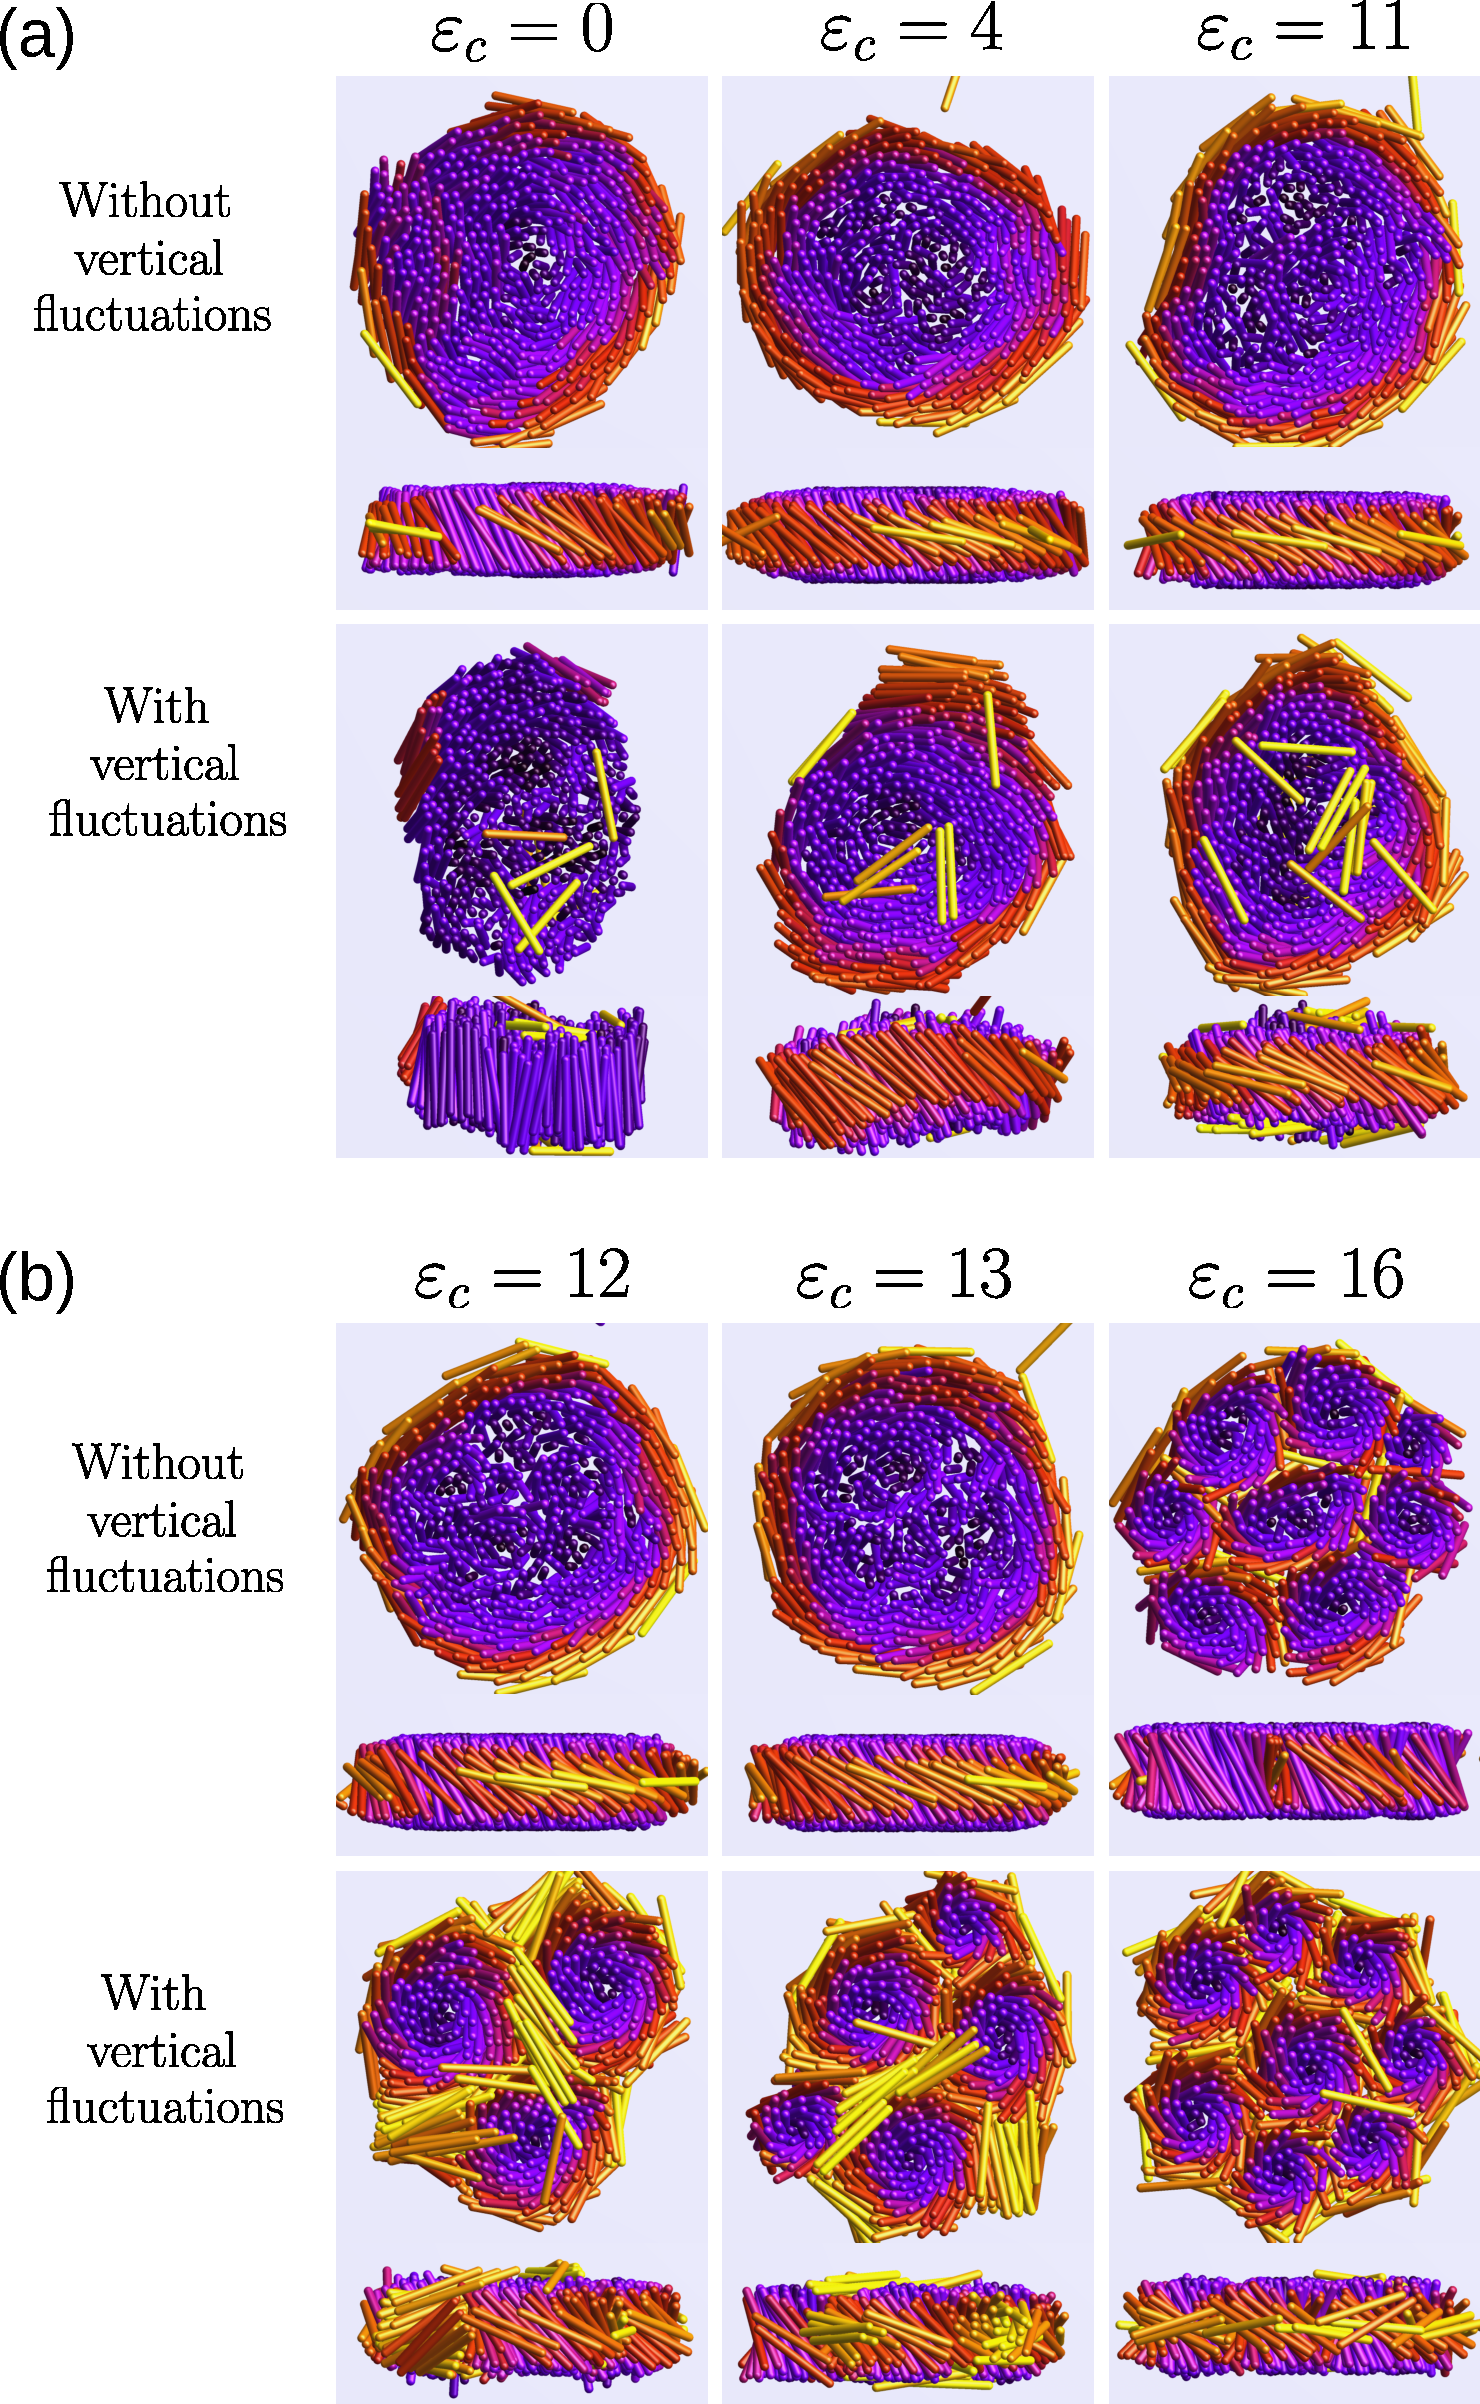
\includegraphics[width= .8\columnwidth]{figures/chapter-5/samples}.
	\caption{Top and front views of membrane-shaped tactoids of chiral rods mixed with non-adsorbing polymer formed in bulk. Color indicates the enclosed angle between each individual rod and the average direction of the system, from black $\varphi = 0$ to yellow $\varphi = \frac{\pi}{2}$. Shared parameters are $a = 2D$, $\ell = 10$ and $N = 500$. For the cases where vertical fluctuations are (not) allowed, $\phi_P=0.25D^{-3}$ ($\phi_P=0.175D^{-3}$).(a) Low chirality regime. (b) High chirality regime.}
\end{center}
\end{figure}


\begin{figure}
\begin{center}
\includegraphics[width= \columnwidth]{figures/chapter-5/crystallinity_11}.
	\caption{ \label{crystal11} Crystallinity of membrane-shaped tactoids of chiral rods mixed with non-adsorbing polymer formed in bulk. Top row: 3D depiction of the system (a) without vertical fluctuations and (b) with vertical fluctuations. Middle and bottom rows: corresponding horizontal sections along the plane generated from a 2D linear regression of the centers of mass of the rods. Upright (untwisted) rods look like disks in this view, while tilted rods appear as ellipses. Color scales indicate: (a)-(c), (f): enclosed angle between the direction of each individual rod and the overall average direction; (d), (g): average distance between each individual rod and its six nearest neighbours; and (e), (h): nearest neighbour distance's standard deviation. Shared parameters are $a = 2D$, $\ell = 10$, $N = 500$ and $\varepsilon_c=11$. For the case where vertical fluctuations are (not) allowed, $\phi_P=0.25D^{-3}$ ($\phi_P=0.175D^{-3}$).}
\end{center}
\end{figure}


\begin{figure}
\begin{center}
\includegraphics[width= \columnwidth]{figures/chapter-5/crystallinity_16}.
	\caption{ \label{crystal16} Crystallinity of multi-domain membrane-shaped tactoids of strongly chiral rods mixed with non-adsorbing polymer formed in bulk. What is illustrated in this figure is equivalent to Fig. \ref{crystal11} except for the chosen chirality regime ($\varepsilon_c=11$ in Fig. \ref{crystal11}, $\varepsilon_c=16$ in this figure).}
\end{center}
\end{figure}


\begin{figure}
\begin{center}
\includegraphics[width= .9\columnwidth]{figures/chapter-5/density}.
	\caption{Rod number density profile of membrane-shaped tactoids of chiral rods mixed with non-adsorbing polymer formed in bulk. Top: without vertical fluctuations. Bottom: with vertical fluctuations. For all cases, $a = 2D$. For the cases where vertical fluctuations are (not) allowed, $\phi_P=0.25D^{-3}$ ($\phi_P=0.175D^{-3}$). } % TODO: explain more.
\end{center}
\end{figure}


\begin{figure}
\begin{center}
\includegraphics[width= .9\columnwidth]{figures/chapter-5/twistprofile}.
	\caption{Twist angle profile of membrane-shaped tactoids of chiral rods mixed with non-adsorbing polymer formed in bulk. Top: without vertical fluctuations. Bottom: with vertical fluctuations. For all cases, $a = 2D$. For the cases where vertical fluctuations are (not) allowed, $\phi_P=0.25D^{-3}$ ($\phi_P=0.175D^{-3}$). } % TODO: explain more.
\end{center}
\end{figure}


\begin{figure}
\begin{center}
\includegraphics[width= \columnwidth]{figures/chapter-5/zstd}.
	\caption{Vertical fluctuations as a function of the distance to the center of 3D membrane-shaped tactoids of chiral rods mixed with non-adsorbing polymer formed in bulk, $a = 2D$, $\phi_P=0.25D^{-3}$. } % TODO: explain more.
\end{center}
\end{figure}





\section{Theory for twisted membranes}




\begin{SCfigure}
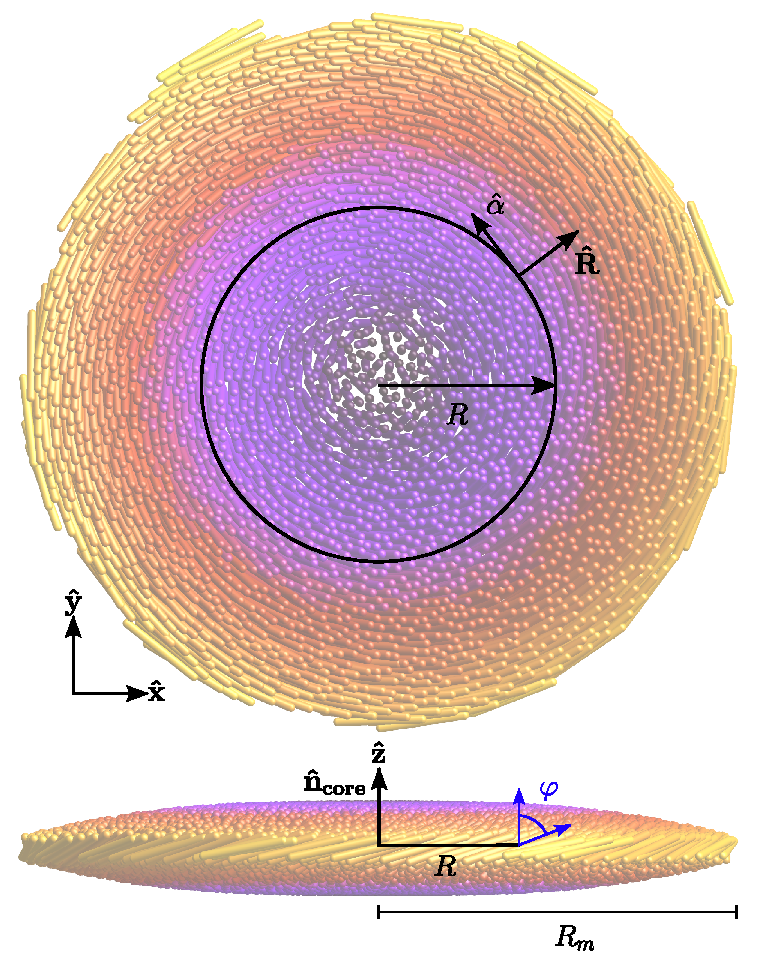
\includegraphics[width= 0.4 \columnwidth]{figures/chapter-5/membrane_sketch}.
\caption{ \label{memsnap} Schematic structure (top and front view) of a twisted smectic membrane of radius $R_{m}$ composed of strongly chiral spherocylinders with aspect ratio $\ell = 10$ mixed with non-adsorbing polymers (not shown) providing strong side-to-side depletion attraction between the rods.  The top graph depict the top view, the lower one a side view of the membrane. The director twist, expressed by the twist angle $\varphi$, is zero at  the membrane  core $\bn _{\rm core} = \bz$ and increases concentrically with radius $R$.}
\end{SCfigure}




 To complement our simulations results we now develop a theory for twisted membranes by focussing on two distinct morphologies that have been observed in experiment, namely half-skyrmion-type membranes and twisted ribbons. In both cases, the twisting of the rods occurs in both principal directions of the membrane (double twist), whereas the cholesteric phase exhibits unidirectional twist. Somewhat confusingly, double twist may also refer to the case of {\em chiral ribbons} in which the membrane itself is wrapped 
in a helical fashion thus exhibiting non-zero mean curvature \cite{green1936equilibrium,chopin2016roadmap}. Although these chiral ribbons have also been observed in {\em fd} polymer mixtures under cetain conditions \cite{Gibaud2014} but we will not consider this particular case in our model. 
 
 
 Let us begin by recalling the well-known Frank-Oseen elastic energy of the general case of a bulk chiral liquid crystal for and arbitrary nematic director field $\bn$ in three spatial dimensions:
\begin{align} 
F = & \frac{1}{2} \int d \bfr \left [ K_{1} (\nabla \cdot \bn)^{2}  + K_{2} (\bn \cdot \nabla \times \bn + q_{0})^{2}  +   K_{3} (\bn \times \nabla \times \bn)^{2} \right ]  
\end{align}
with $K_{1}$, $K_{2}$ and $K_{3}$ respectively denoting the splay, twist and bend elastic moduli.   The inverse  pitch  $q_{0}$ quantifies the chiral strength of the particles in the liquid crystal. 


 For the specific case of a cylindrically symmetric, twisted membrane depicted in\fig{memsnap}
  with radius $R_{m}$ we may invoke a cylindrical geometry  with radial coordinate $0<R< R_{m}$ and angle $\alpha$.  Deformations from a uniform director field in which case $\bn = \bz$ are assumed to be concentric and can be described as:
 \beq
 \bn = \cos \psi (R) \cos  \varphi(R) \bz + \cos \psi (R) \sin \varphi(R) \bal + \sin \psi(R) \bars
 \label{tilt}
 \eeq
in terms of a twist angle  $ \varphi $ denoting a twist deflection of the rods with respect to the membrane normal and $\psi$ a splay deformation along the membrane radial vector (see \fig{memsnap}).   We the local rod density within the membrane to be uniform so that the one-body density reads $\rho(R, \bw)  = \rho_{0}f(R,  \bw)$, in terms of the rod number density $\rho_{0}$ denoting the number of rods per area unit, and a three-dimensional rod unit vector $\bw$ distributed along the local director obeying an a priori unknown distribution $f$. The twist-bend elastic free energy  takes the following form \cite{barry_jpcb2009,wensink2018elastic}:
\begin{align}
 F_{el}  &= \int  d \brr \left [ K_{2} \left ( \partial_{R} \varphi + \frac{\sin 2 \varphi}{2R} + q_{0} \right )^{2}  + K_{3}\frac{ ( \sin \varphi )^{4}}{R^{2}} \right   ]
\label{fmem}
\end{align}
with $\int d {\bf R} = 2 \pi \int_{0}^{R_{m}} R dR $ in circular coordinates for a membrane with radius $R_{m}$.
 The  elastic moduli for the membrane are distinctly different from those of a ulk liquid crystal and will be specified in the next section. We remark that these elastic moduli are strictly 2D quantities with dimension energy.  


In an earlier version of our theory \cite{wensink2018elastic} the effect of depletion attraction due to the non-adsorbing polymer can be described in terms of a simple free energy 
\beq
F_{dep}  \sim U_{0} \int d \brr  (\sin \varphi )^{2}  + {\rm cst}
\eeq
where $U_{0}$ is a tilt energy density (per unit area) related to the osmotic pressure of the polymer reservoir and polymer radius of gyration. The simple sine squared contribution is chosen here for simplicity and is in line with de Gennes' original treatment of twist expulsion towards the edges or around defects of smectic layers in analogy with superconductors \cite{gennes-prost, barry_jpcb2009}. It captures the basic trend that the local director tilting away from the membrane normal compromises the free volume experienced by the non-adsorbing polymer  thereby inducing a free energy penalty. In our theory, out-of-plane fluctuations of the rod centre-of-mass away from the 2D plane are not included, but this can be done so on a simple mean-field level \cite{kang_sm2016}.
Ignoring the curvature terms  $R \rightarrow \infty $ and considering a smectic layer on an infinite half-plane enables an analytical minimisation of the free energy in terms of the twist penetration depth $\lambda_{t}  =  \sqrt{K_{2}/a} $ \cite{gennes-prost,barry_jpcb2009}. For the circular membrane, a simple simulated-annealing Monte Carlo algorithm can be employed to minimise the free energy with respect to the twist angle $\varphi(R)$ for any given triplet of length scales, namely the bulk cholesteric pitch $q_{0}^{-1} $, twist penetration depth $\lambda_{t} $ and membrane radius $R_{m}$. With the twist elastic modulus and chiral amplitude being microscopically defined \eq{kexp} a simple one-parameter fitting procedure can be used to determine the depletion strength $a$ and the twist penetration depth $\lambda_{t}$. 



 The main features we established from the numerical results \cite{wensink2018elastic} are the following:  (i) the twisting becomes more pronounced toward the membrane edge when the twist penetration depth becomes shorter, as expected,  but also when membrane size grows larger. (ii) Increasing the pitch $q_{0}$  enhances the maximum twist angle while keeping the overall shape of the twist angle profile largely unchanged. (iii) The local splay angle remains negligibly small  across the membrane so that the omission of splay effects seems fully justified.




\subsection{Scaling results for the elastic moduli for a fluid membrane}

Using second-virial theory combined with a Gaussian approximation for the orientation probability of the rods within the membrane one can estimate the leading-order contributions of the torque-field, splay, twist and bend elastic constants of a membrane, respectively:
\begin{align}
  K_{1}   & \sim  \frac{17 \rho_{0} \ell^{2}}{24} = \frac{17}{2} K_{2}   \nonumber \\ 
 K_{2}  & \sim  \frac{\rho_{0} \ell^{2}}{12}   \nonumber \\ 
 K_{3} &\sim  \frac{1}{4} K_{2}
  \label{kexp}
\end{align}
Note that the membrane moduli have unity ${\rm N \cdot m}$ (the 3D moduli would be expressed in Newtons) and $\rho_{0} = ND^{2}/A$ refers to planar density of rods with diameter $D$, aspect ratio $\ell = L/D$ and membrane area $A$. The results suggest that the moduli of rodlike particle confined to a membrane are quite different from those of of 3D bulk nematic fluid, at least for strongly elaongated rods experiencing strong nematic order.  In the limit of asymptotic alignment, the splay-to-twist ratio of a bulk fluid  \cite{odijkelastic}  was predicted to scale as $K_{1}/K_{2} \sim 3 $ whereas a much higher ratio $K_{1}/K_{2} \sim 17/2$ is found for the membrane. The bend-to-twist ratio for a hard rod nematic fluid was found to be proportional to the degree of nematic alignment $K_{3}/K_{2} \sim \sigma \gg 1$ \cite{odijkelastic} where $\sigma$ is steered by the rod concentration.  The curvature-to-twist elasticity of a membrane turns out to be smaller than unity $K_{3}/K_{2} \sim 1/4$ and independent of the rod concentration.  In other words, rods confined to a membrane experience a much stronger resistance to splay fluctuations whereas  bend fluctuations are far less penalised compared to a 3D nematic fluid.  Since the splay modulus is about an order of magnitude larger than the twist elasticity, we expect director deformations whereby rods tilt along the radial vector of the membrane to be of marginal importance and  will be ignored.  





\subsection{Chiral twist }

The pitch $q_{0}$ of a twisted membrane can be estimated by considering a weakly chiral pair potential $U_{c}$ described by some arbitrary but short-ranged spatial decay function $g(r)$ describing the range over which chiral forces interact and chiral amplitude $\varepsilon_{c} $ much smaller than the thermal energy. This potential takes the following generic form \cite{goossens1971}:
\beq
U_{c} \sim  \varepsilon_{c} g( r)(\bwa \times \bwb \cdot   \bx) (\bwa \cdot \bwb)
\label{uchi}
\eeq
From this, we may compute the so-called torque-field constant exerted by the chiral potential \cite{wensink2018elastic}:
\beq
K_{t}   \sim -\rho_{0}^{2}  \bar{\varepsilon}_{c} 
\eeq
in terms of an integrated chiral amplitude  $\bar{\varepsilon}_{c}$ which is  {\em different} from that of a  3D cholesteric system as it implicitly encodes the geometric confinement given that $\bdr$ is a 2D vector:
\beq
 \bar{\varepsilon}_{c}  =  \varepsilon_{c} \int d \bdr | \bdr \cdot \bx |    g( r)
 \eeq
 which has units energy times volume ($k_{B}T \times D^{3}$). The chiral potential drives the twisting of the membrane and $K_{t}$  provides an explicit link between the effective torque-field and the range and amplitude  of the chiral pair potential between a pair of  rods. We remark that the above mean-field treatment will be less adequate for strongly chiral amplitudes $\varepsilon_{c} \gg k_{B}T$. A common choice for $g(r)$ is a short-ranged power law $g(r) = 1/r^{7}$ but  long-ranged forms such as a square-well (SW) potential could be conceivable as well \cite{wensinkjackson}. Taking the power law featuring in \eq{uchiral} we obtain $\bar{\varepsilon}_{c} = \varepsilon_{c} D^{3}$.  From this we find a {\em microscopic} expression for the typical equilibrium  pitch of the membrane $q_{0} = K_{t}/K_{2}$ that further depends on the in-plane rod density $\rho_{0}$ and rod aspect ratio $\ell = L/D$:
 \beq
 q_{0} \sim \frac{12 \rho_{0} \bar{\varepsilon_{c}}}{ \ell^{2}}
 \label{qzero}
 \eeq
 While for the singletwisted cholesteric phase the twist angle increases linearly  $\varphi(z) = q_{0} z$ at each position $z$ along the helix axis, the angle will be strongly non-linear with radius $R$ in case of the twisted membrane, in particular if the twist penetration length $\lambda_{t}$ is small \cite{wensink2018elastic}.   
 


\subsection{Effect of depletants and twist penetration length}

Kang et al. \cite{kang_sm2016} have proposed a more sophisticated expression for the effect of the depletion attraction on the twist angle via the local membrane height $h = (L/2) \cos \varphi$: 
\begin{align}
F_{dep}  \sim & 2 n_{p} a k_{B}T \left [ \int  d {\bf R} \sqrt{ 1 + (\nabla h)^{2} } + \oint d {\bf l} h \right ]
\label{fdep1}
\end{align}
with $n_{p}$ the polymer reservoir pressure and $a$ the polymer radius of gyration. The last contribution is identified a line tension generated by depletion forces between rods. Combining this with the elastic part of the 
\eq{fmem} we find the following free energy for a membrane with radius $R_{m}$:
\begin{align}
\frac{ F}{K_{2}}  &\sim \int  d \brr   \left [  \left ( \partial_{R} \varphi + \frac{\sin 2 \varphi}{2R} + q_{0} \right )^{2}  + \frac{K_{3}}{K_{2}}\frac{ ( \sin \varphi )^{4}}{R^{2}} \right . \nonumber \\ 
& \left .  + \lambda_{t}^{-2}    \sqrt{ 1 + (\partial_{R} h)^{2} }   \right ]  + 2 \pi  \lambda_{t}^{-2} R_{m} h(R_{m})
\label{fmem1}
\end{align}
with $\int d {\bf R} = 2 \pi \int_{0}^{R_{m}} R dR $ in circular coordinates. The line tension contribution drops with increasing twist at the edges and  becomes zero if the rods are twisted perpendicular to the membrane normal $\varphi(R_{m}) = \pi/2$. 
The twist penetration length is given by $\lambda_{t} = \sqrt{K_{2}/2  n_{p} a k_{B}T}$ which, using \eq{kexp} leads to a compact expression depending on quantities known from experiment such as the in-plane rod density (assumed uniform across the membrane), rod-polymer size ratio $D/a$, rod aspect ratio $\ell$ and the reservoir polymer concentration $n_{p}$: 
\beq
\frac{\lambda_{t}}{D} = \sqrt{\frac{\rho_{0} \ell^{2} }{24  (n_{p} a^{3}) (D/a)^{2} }}
\eeq
Taking typical numbers from our simulation ($\ell \sim 10$, $\rho_{0} \sim 0.5$, $D/a=2$ and $n_{p}a^{3} \sim 0.2$) we find that that the twist penetration length is only a few times the rod diameter, i.e. $\lambda_{t} \sim 2 D$. 
For {\em fd} rods a much larger value is found primarily because they are longer than our rods ($\ell \sim 130$). The predicted value $\lambda_{t} \sim 20 D$ is roughly line with the experimentally measured value of about half a rod length   depending on the polymer concentration that was used to stabilize the membranes \cite{barry_jpcb2009}.

In Ref. \cite{kuhnhold2022colloidal} a simple trial form was used to fit the simulation data:
\beq
\varphi(R) = \varphi_{0} \left ( \frac{R}{R_{m}} \right )^{\alpha} 
\eeq
with $\varphi_{0}$ the twist angle at the membrane edge and $\alpha $ a variational parameter governing the degree of twist near the edge.  It is tempting to insert the trial form into the free energy \eq{fmem1} and seek an algebraic minimization route through the variational parameters $\varphi_{0}$ and $\alpha$.   However, such an approach turns out to be too unfeasible because the free energy is strongly non-linear in $\varphi$.  As in Ref. \cite{wensink2018elastic} we therefore employ a simulated-annealing Monte Carlo algorithm to obtain the angular profile as a function of the distance from the membrane core. 

\section{Starfish instability and twisted ribbon}


\begin{figure}
\begin{center}
\includegraphics[width= \columnwidth]{figures/chapter-5/ribbon_sketch}.
\caption{ \label{ribsnap} Schematic structure of of twisted ribbon of width $s_y=2\ell$ composed of strongly chiral spherocylinders with aspect ratio $\ell = 15$ mixed with non-adsorbing polymers (not shown) providing strong depletion attraction between the rods. The rods are color coded by orientation.  }
\end{center}
\end{figure}

At elevated chiral strength the circular membranes are known to transition into twisted ribbons \cite{Gibaud2014}. These were identified as quasi-1D twisted protrusions growing out of the perimeter of the membrane, through a mechanism termed `starfish' instability. 


Lowering the temperature strengthens the chiral forces between the rods, which raises the free energy of the interior untwisted rods while lowering the free energy of edge-bound twisted rods. This enables chiral control of edge line tension which, when the edge tension approaches zero,  leads to spontaneously transitions of the membrane into an array of 1D twisted ribbons, called a ‘‘starfish’’ \cite{Gibaud2014}. A phenomenological model aimed at capturing the onset of the surface-driven instability was presented in Ref. \cite{kang_sm2016}.




We may adopt the same reasoning we applied to the membrane and formulate a free energy for a ribbon, depicted in \fig{ribsnap}. While the membrane exhibits double twist in a circularly symmetric fashion, the rods within the ribbon are twisted in two mutually perpendicular directions along the short and long axes of the ribbon.  Then, the director field of a twisted ribbon may be constructed from a combination of two rotation matrices, each corresponding to a twist along mutually perpendicular Cartesian axes. Without loss of generality we fix the director field of the untwisted ribbon along the $x$-axis of the frame $\bn_{0}=(1,0,0)$ so that the director field of the ribbon reads: 
\beq
\bn_{r}[ \Phi, \chi] = \mathcal{R}_{xz} [\Phi]\cdot \mathcal{R}_{xy}[\chi] \cdot \bn_{0}
\label{nrib}
\eeq
in terms of the rotation matrices
 \beq
 \mathcal{R}_{xz} [ \Phi]   =
  \begin{bmatrix}
     \cos \Phi(y) & 0 & \sin \Phi(y)  \\
    0 & 1 & 0  \\
    -\sin \Phi(y) &  0 & \cos \Phi(y)  \\
      \end{bmatrix}  \nonumber
      \label{rxz}
 \eeq
and
 \beq
 \mathcal{R}_{xy} [ \chi]   =
  \begin{bmatrix}
     \cos \chi(z) &  \sin \chi(z) & 0  \\
    -\sin \chi(z) &   \cos \chi(z) & 0 \\
      0 & 0 & 1  \\
      \end{bmatrix}  \nonumber
      \label{rxy}
 \eeq
Here, $\Phi$ and $\chi$ denote  two  angles describing the twist along the short and long (ribbon) axes that we parameterize via the coordinates $-s_{y}/2 < y < s_{y}/2$ and $-s_{z}/2< z <s_{z}/2$, respectively. The ribbon area $A = s_{y}s_{z}$ is conserved. We further define the local thickness of the ribbon:
\begin{align}
h = \frac{L}{2}   | \bn_{0} \cdot \bn |  =\frac{L}{2} |\cos \chi(y) \cos \Phi(y)| 
\end{align}
We now simplify matters by assuming linear twist in both directions so that $\chi = qz$ and $\Phi = qy$ where $q$ denotes the principal pitch of the ribbon quantifying the degree of twist along the long and short ribbon axes. We remark that the  ribbon pitch is likely to be different from the value $q_{0}$ that we defined in \eq{qzero} which quantifies the chiral strength between the rods. Henceforth, we will use the ribbon width as our length unit and render all pitches dimensionless via $q \rightarrow q s_{y}$. We assume the ribbon to be long eough so we can ignore surface effects imparted by the short edge of the ribbon. Using the parameterization of the director \eq{nrib} we find that the   contributions corresponding to bend, splay and twist elasticity {\em per unit ribbon length}  reads:
\begin{align}
F_{bend} &=\frac{K_{3}}{16} \left [ 3 q^{2} - q \sin q (\cos q -2)\right ]  \nonumber \\ 
F_{splay} &=  
\frac{K_{1}}{8}  (q^{2}  - q \sin q )  \nonumber \\ 
F_{twist} &=  \frac{K_{2} }{16  }  \left [ 8 q_{0}(q_{0} -q -\sin q)  + q\sin q ( \cos
   q +4) + 7 q^{2}\right ]
\end{align}
Note that the bulk elastic energies   are all {\em even} functions of the pitch $q$, expect the first term in the twist contribution which encodes chirality and vanishes for achiral rods ($q_{0} =0$). 
 We must also consider the effect of saddle-splay, which is nonzero due to the curvature of the ribbon (it does not play a role for the flat membranes). It can be defined in terms of the following bulk contribution to the Frank elastic energy: 
\beq
F_{saddle} = -\frac{K_{24}}{2} \int d \bfr   [\nabla \cdot ( \bn \nabla \cdot \bn +  \bn \times \nabla \times \bn )]
\eeq
which gives:
\beq
F_{saddle} = -\frac{K_{24} }{4 }  q \sin q
\eeq
The depletion contribution \eq{fdep1} can be derived in a similar way. Ignoring factors independent of the pitch, we find:
\begin{align}
F_{dep}  & \sim  2 n_{p} a k_{B}T \left  [  \frac{(qL)^{2}}{16}  + \oint d \ell h \right ] 
\end{align}
Twisting a rectangular slab into a ribbon enhances the contour length of the object, which is reflected in the line integral in \eq{fdep1} that we express as $\oint d {\bf l}h = (q/2 \pi)\sqrt{1+ (q/2)^{2}}\int_{-\pi/q}^{\pi/q} dz h$. With this we find a simple expression:
\beq
 \oint d {\bf l} h  = \frac{2L}{\pi} | \cos  (\tfrac{1}{2} q) |    \sqrt{1+ \tfrac{1}{4} q^{2}} 
\eeq
which suggests  that the  tension contribution is minimal at maximum tilt at the ribbon edge when $q = \pm \pi $. Simultaneously, it penalizes large pitches as the perimeter-to-area ratio of the ribbon increases with the degree of longitudinal twist, although this effect is of minor importance.  



Although the expressions obtained are entirely algebraic,  minimization of the total free energy can only be performed numerically. To make progress, we  expand the free energy contributions up to quadratic order in $q$.
Combining terms and reintroducing the twist penetration length $\lambda_{t}$ we arrive at a compact expression for the total free energy per unit length of a weakly twisted ribbon ($q \ll 1/s_{y}$): 
\beq
\frac{F}{K_{2}} \sim   -q q_{0}   +  \frac{1}{2}\left ( \frac{\Delta K}{2} + \frac{L^{2}}{8\lambda_{t}^{2}}\right )  q^{2} + \frac{2 L }{\pi \lambda_{t}^{2}}
\label{flowq}
\eeq
The first two term encodes the free energy change due to (chiral) twist, the second  the effect of splay, bend and saddle-splay elasticity along with depletion, whereas the last term denotes the line tension which up to leading order does not depend on the pitch.  The constant $\Delta K$ represents a combination of the  bend-twist and saddle-twist elastic anisotropies:
\beq
\Delta K = \frac{K_{3}}{K_{2}} - \frac{K_{24}}{K_{2}} + 3
\label{dk}
\eeq
The equilibrium ribbon pitch follows from minimizing \eq{flowq} and is related to $q_{0}$ via:
\begin{align}
q & \sim q_{0} \left ( \frac{\Delta K}{2} + \frac{L^{2}}{8\lambda_{t}^{2}}\right )^{-1}  
\end{align}
Inserting this back into the quadratic free energy and reexpressing all variables in bare units we find:
\beq
\frac{F}{K_{2}} \sim -\frac{1}{2} \left ( \frac{\Delta K}{2} + \frac{L^{2}}{8\lambda_{t}^{2}}\right ) (q_{0} s_{y})^{2} + \frac{2 Ls_{y} }{\pi \lambda_{t}^{2}}
\eeq
which combines a bulk term proportional to $s_{y}^{2}$ and a surface contribution  linear in $s_{y}$. Minimization yield for the typical ribbon width:
\beq
s_{y} \sim \frac{2 L }{ \pi \lambda_{t}^{2} q_{0}^{2} } \left ( \frac{\Delta K}{2} + \frac{L^{2}}{8\lambda_{t}^{2}}\right ) 
\eeq
Finally, we deduce  the ribbon pitch versus width:
\beq
\frac{\textrm{ribbon pitch}}{\textrm{ribbon width}} = \frac{2 \pi}{q s_{y}} \sim  \frac{\pi^{2} q_{0} \lambda_{t}^{2} }{L}
\eeq
and the tilt angle at the ribbon edge:
\beq
\Phi(s_{y}) = \frac{1}{2} q s_{y} \sim \frac{L}{\pi q_{0} \lambda_{t}^{2}}
\eeq
The predictions above should be qualitatively correct and give valuable insight into how the ribbon properties depend on the intrinsic chirality and elasticity of the LC material.  A potential caveat of the low-$q$ expansion, however, is that ribbons form at elevated chirality where the ribbon pitch $qL$ is not necessarily a small parameter ($qL \ll 1$). Because deviations from the simple quadratic free energy \eq{flowq} are to be expected, we chose to minimize the free energy numerically which is an easy task given that all free energy contributions  are in  algebraic form.

In doing so, we  also probe a more general scenario where the twist along the principal ribbon directions is {\em anisotropic}. To this end, we characterize  the twist angles  via $\chi = q_{\parallel} z$ and $\Phi = q_{\perp}y$ in terms of a longitudinal and transverse pitch, $q_{\parallel}$ and $q_{\perp}$, respectively. 
 Typical input values  for the case of {\em fd} rods can be obtained by fixing the twist penetration length $\lambda_{t}  = L/2$ \cite{barry_jpcb2009} and taking a typical (cholesteric) pitch $q_{0} = 0.4L^{-1}$. The elastic anisotropy $\Delta K$ is much harder to specify as it depends quite sensitively on the  saddle-splay modulus $K_{24}$ which is unknown for {\em fd} rods. 

The numerical results are shown in \fig{fig3}.  In general, we find that the ribbon pitch is larger than  the pitch $q_{0}$ quantifying the degree of twist the membrane or cholesteric phase. We further predict that the ribbon width is always just a few times the rod length, suggesting that ribbons are indeed very slender quasi 1D  objects, while the pitch-to-width ratio is of $\mathcal{O}(1)$, in agreement with  experimental observations reported in Ref. \cite{Gibaud2014}. 


\begin{figure}
\begin{center}
\includegraphics[width=  0.7 \columnwidth]{figures/chapter-5/deltak}.
\caption{ \label{fig3} Overview of the ribbon width $s_{y}$ and pitch $q$ as a function of the elastic anisotropy $\Delta K$ [\eq{dk}] of the LC material. Parameters $\lambda_{t} = 0.5 L$ and $q_{0} = 0.4 L^{-1}$. }
\end{center}
\end{figure}

 

%where  $q \ll q_{0}$ depending on the elastic anisotropy and twist penetration length. We remark that the ribbon pitch does not depend on the line tension (second term in \eq{flowq} which is independent of $q$).  

% Check minimize free energy per pitch versus per unit length = 2pi/qq. Combined minimization wrt qq and sy by reverting free energy to bare units rod length.



%Before proceeding with our analysis we immediately infer a couple of basic facts from inspecting \eq{fribbon}. First, as expected chiral forces between the rods, represented by the term proportional to $2-\tau^{2}$, lower the free energy provided the ribbons are sufficiently elongated ($\tau  >\sqrt{2})$. A further stabilization mechanism occurs through the line tension since the curvature correction $w_{2}$ is negative. 

%The relevant constants $\Delta K$ and $\Delta \ell$ can be estimated from the twist penetration length. Taking the reference value $\lambda_{t} = L/2$ quoted for {\em fd} virus rods we find that  $\Delta K \sim (L/2\lambda_{t})^{2} \sim 1 $,  ignoring weak contributions from the bend-to-twist and saddle-splay elasticity. Similarly, we obtain $\Delta \ell \approx 4 $ for a ribbon with a lateral width equal to the rod length $s_{y} = L$. For the pitch we roughly estimate $q_{0} = 2 \pi s_{y} / p_{c} \approx 0.2$ taking a cholesteric pitch  $p_{c} \sim 30L$. 

%The next step is to minimize the free energy \eq{fribbon} with respect to the ribbon pitch $q$ and aspect ratio $\tau$, i.e., $\partial F/\partial q =0$ and $\partial F/\partial \tau =0$ for a given ribbon area $A$. If the line tension is ignored ($\Delta \ell =0$), the extremum condition can be solved analytically and gives an equilibrium ribbon pitch:
%\beq
%q =  \frac{3q_{0}}{4 \Delta K} \frac{(\tau^{2} -2)}{1 + \tau^{2}}
%\eeq
%where the last contribution is a monotonically increasing function for $\tau^{2} >2$ levelling off to unity for $\tau \gg 1$. The ribbon free energy per unit area corresponding to the optimal pitch is:
%\beq
%\frac{F/\tau}{K_{2}}  = -\frac{1}{96} q_{0}  (\tau^{2} -2) q^{3}
%\eeq
%From this we infer that (i) stable ribbons that are not curbed by line tension penalty tend to stretch to very large aspect ratios, and (ii) the limiting pitch at large ribbon aspect ratio is likely smaller than the membrane pitch $q_{0}$ given that $q =  3q_{0}/4 \Delta K$ for $\tau \rightarrow \infty $ and $\Delta K \sim 1$. In practice, conservation of area precludes the ribbons to stretch to infinity while a finite line tension puts a further natural bound to $\tau$. 



%\subsection{Effect of anisotropic twist} 

%\begin{figure}
%\begin{center}
%\includegraphics[width=  0.5 \columnwidth]{figures/chapter-5/raniso}.
%\caption{ \label{fig3} Twist anisotropy $\gamma$ and pitch $q$ of a twisted ribbon with width $s_{y} = L$ as a function of the %ribbon length $\tau$. The chiral strength between the rods is given by the membrane pitch $q_{0} = 0.2L^{-1}$ (horizontal black %line). The twist penetration length is $\lambda_{t} = 0.5L $.   }
%\end{center}
%\end{figure}


%Let us now explore the possibility of unequal twist along the short and long ribbon axes. This should render a more realistic picture of the internal twist profile of the ribbon  given that the twist along the principal ribbon directions need not have the same magnitude. We proceed by allowing $\gamma$, which denotes the ratio between the degree of twist along the long and short axes  of the ribbon,  to be a  variable quantity. Working out the algebraic free energy per area we find for the bulk elastic contribution:
%\begin{align}
%\frac{F}{ K_{2} \tau} &\sim 
%\frac{1}{24} \left [ \frac{K_{3}}{K_{2}} q^{4} (1 + \tau^{2}) \gamma^{2} + B\right ]
%\end{align}
%with $B$ the twist elastic contribution:
%\beq
%B = (q_{0} + q - q \gamma) (12 q_{0} + q (12 - \gamma (12 + q^2 ( \tau^{2} \gamma -2))))
%\eeq
%This term reduces to the much simpler expression explored in the previous section for the isotropic twist case ($\gamma =1$). Similarly, the saddle-splay term now becomes:
%\beq
% \frac{F}{K_{2} \tau} \sim  - \frac{1}{24}\frac{K_{24}}{ K_{2} } q^{4} \gamma (1 + \tau^{2} \gamma)
%\eeq
%Finally the depletion free energy reads (ignoring irrelevant constants as well as the line tension contribution):
%\beq
% \frac{F}{K_{2} \tau} \sim  \frac{L^{2}}{96 \lambda_{t}^{2}} q^{4} (1 + \tau^{2} \gamma^{4})
%\eeq
%Clearly, these complex expressions are no longer amenable to further analytical treatment. Furthermore, the elastic and depletion strengths can longer be compactly combined into a  single parameter $\eq{dk}$ as could be done for the isotropic twist case but must be  separately defined. However, minimization of the three free energy terms above with respect to $q$ and $\gamma$ is easily carried out numerically and the results are shown in \fig{fig3} taking $K_{3}/K_{2} = 1/4$, $q_{0} = 0.2$, $\lambda_{t} = L/2$ and three different values for the saddle-splay elastic modulus. Clearly,  $\gamma $ tends to be larger than unity depending on the strength of the saddle-splay elasticity $K_{24}$ indicating twisting along the main ribbon axis can be about 30-50 \% stronger than across the short axis. We remark that $K_{24}$ plays an essential role in driving the  twist for the ribbon geometry. In fact, saddle-splay elasticity cannot be ignored given that  no physical solutions of the minimization problem were found  for $K_{24} =0$. The lowest value explored ($K_{24} = K_{2}/2$) roughly recovers the previous scenario of equal twist along the short and long ribbon axes. The fact that a positive value of the $K_{24}$ is required for stabilizing ribbons is consistent with the work of Kaplan {\rm et al.} \cite{kaplan2010theory} providing a more wide-ranging theoretical framework for membranes and ribbons  based on a Helfrich-DeGennes model which also considers the effect of layer bending (ignored in our model).  

%We further conclude from \fig{fig3}b that longer ribbons tend to be less twisted than short ones.   Short ribbons ($\tau <10$) seem {\em overtwisted} compared to that of the equivalent (single twist) cholesteric phase while long ribbons experience less twist. In all cases we see that $q$ levels off to a limiting value $q < q_{0}$ for infinitely stretched ribbons ($\tau \rightarrow \infty$) in line with our analytical predictions for the case of constrained isotropic twist $\gamma =1$. The line tension, ignored in the results of \fig{fig3}, will put a constraint on the optimal aspect ratio $\tau$ which needs to optimized along with $q$ and $\gamma$ for a given ribbon area. We will not pursue this further in this study given that, in experiment, the line tension at the starfish transition is very low while the available virus material and hence the area tends to be quite large. Both  factors enable these ribbons to grow into strongly elongated objects. This should be compared to our predictions for the limiting case $\tau \rightarrow \infty$. Further restriction  to applying our model to experiments relates to the unknown saddle-splay constant for {\em fd} virus rods. 

%A further characteristic we may deduce from our model is the typical long-axis pitch, in the experiments simply referred to as the pitch,  versus ribbon width.  This ratio of length scales is given by:
%\beq
%\frac{\textrm{ribbon   pitch}}{\textrm{ribbon width}} \sim \frac{2 \pi}{\gamma q s_{y}} 
%\eeq
%From the optical microscopy pictures provided in Ref.  \cite{Gibaud2014} we roughly infer that this ratio should be about 2-3. Taking ribbons of moderate length, say  $\tau = 5$, we find that the predicted ratio is somewhat larger ($\sim 10$), in qualitative agreement with experimental observation.




\section{Conclusions}




\clearpage








 % Cholesterics: collective effects

\chapter{Morphology of strongly confined tactoids of colloidal rods stabilized by \\
polymer depletion}
\chaptermark{Morphology of strongly confined tactoids}

\section{Background}

Elongated colloids such as, for example,  filamentous {\em fd} rods, mixed with non-adsorbing polymer form compact tactoids due to the strong depletion attractions experienced by the rods. The size and concentration of the polymer can be exploited to  tune the morphology and internal structure of the droplets. Further complexity can be achieved by the presence of strong geometric confinement.  In our study we consider a slab geometry with width comparable to the rod length. The confinement is expected to generate tactoids with a strongly non-uniform rod density whose morphology is further controlled by strong electrostatic and chiral twist between the individual rods as well as by a surface tension that strongly depends on the average rod orientation with respect to the surface normal. In fact, the presence of the wall imparts a wall-liquid surface tension which is likely to be different from the liquid-gas surface tension which would dominate in the bulk case.

We study these systems by means of Monte Carlo simulations in the semi-grand canonical ensemble ($N,V,\mu_{p},T$) consisting of a system of $N$ rods in a volume $V$ at constant temperature $T$ in osmotic equilibrium with a polymer reservoir at constant chemical potential $\mu_{p}$. The number of polymers  $N_{p}$ in the system is then a fluctuating quantity with the average polymer concentration controlled by $\mu_{p}$.

\section{Model}

We consider a system of $N$ rigid spherocylinders of length $L$, thickness $D$ and aspect ratio $L/D= 10$. The spherocylinders are a simplified representation of {\em fd} rods that are much thinner ($L/D > 100$) and carry a small degree of backbone flexibility with persistence length $\ell_{p} \gg L$. Since the large particle aspect ratio in combination with backbone flexibility poses considerable limitations on the numerical efficiency of our simulations  we  only consider rigid rods with a relatively short length assuming that the key features of the confined tactoids do not  critically depend on the rod aspect ratio or flexibility.

The spherocylinders are mixed with non-adsorbing polymers that in our model act as non-penetrable hard spheres with diameter $\sigma$ equalling once or twice that of the spherocylinder ($\sigma = D$ or $2D$). Polymer-polymer interactions are zero, while the interaction between a polymer and a spherocylinder are treated as being strictly hard;  the potential energy is infinitely large when a  sphere and spherocylinder overlap and zero otherwise.



\begin{figure}
	\includegraphics[width = 0.5 \columnwidth]{figures/chapter-6/spheromans}
	\caption{ Sketch of the simulation model: hard spherocylinders (grey) mixed non-penetrable polymers (blue) with diameter $\sigma = D$ (as depicted here) confined in a slab geometry with wall-to-wall distance $h$. Overlap of the cores (grey) gives infinite repulsion while overlapping coronae (blurred zones) favors a twisted pair configuration representing the (chiral) electrostatic forces between {\em fd} rods. Note that our model is defined in three spatial dimensions. }
	\label{sketch}
\end{figure}



The pair interaction $U_{r}$ between two spherocylinders with solid angles $\oma$ and $\omb$ and centre-of-mass distance $\Delta \bfr$ follows from a combination of short-range steric forces (treated as strictly hard) and electrostatic forces at larger distance. The  interaction potential between a pair rods depends on centre-of-mass distance vector $\Delta {\bf r}$ and orientation vector $\oma$ of both rods. In our model, the interactions are encapsulated in the following core-shell potential:
\beq
U_{\rm r} (\Delta {\bf r}, \oma, \omb) =
\begin{cases}
\infty & \textrm{if hard cores overlap}\\
U_{\rm twist} & \textrm{otherwise} \\
\end{cases}
\label{urod}
\eeq
The electrostatic interactions between {\em fd} rods gives rise to so-called electrostatic twist which is intimately linked to the chirality surface architecture of {\em fd} virus rods. The chiral  potential is commonly expressed in terms of a pseudoscalar form initially put forward by Goossens:
\beq
U_{\rm twist} (\Delta {\bf r}, \oma , \omb )=
-\varepsilon_{c} \left ( \frac{D}{\Delta r} \right )^{7}(\oma \cdot \omb)(\oma \times \omb \cdot \Delta \hat{\bf r})
\eeq
where  $\Delta \hat{\bf r} $ denotes a unit vector for the centre-of-mass distance.
 The sign of $\varepsilon_{c}$ defines the microscopic handedness of the rods. Without loss of generality we take $\varepsilon_{c} > 0$ reflecting the right-handedness of {\em fd} rods. The chiral symmetry of the potential is expressed by the pseudoscalar that imparts a sign change upon  inversion $\Delta \hat{\bf r} \rightarrow - \Delta \hat{\bf r}$. In view of its rapid decay with $\Delta r$ the potential is very short-ranged and the rods need to be very close together in order to feel the chiral twist.

 %For simplicity, we assume that the twisting forces are sufficiently short-ranged (which should be the case at sufficient ionic strength) and do not  continuously vary with the centre-of-mass distance between the spherocylinders, but are only operative if the coronae between the rods overlap (see \fig{sketch}).


 The typical attraction energy between two rods due to polymer depletion can be estimated from free-volume theory \cite{lekkerkerker2011depletion} and reads:
 \beq
 U_{\rm r,dep} \sim -\Pi_{P} V_{\rm r, ov}
 \eeq
with $ \Pi_{P} = k_{B} T N_{P}/V$ the (van 't Hoff) osmotic pressure of the polymer reservoir and $V_{\rm r, ov}$ the overlap volume  of the depletion layers surrounding each rod which depends on the orientation of each rod. In case the rods are perfectly parallel and at hard-core contact we find a simple analytical result. Ignoring  finite rod size effects we have:
\beq
V_{\rm r, ov} = LD^{2} \left [  2 r^{2} \cos^{-1} \left ( \tfrac{1}{2r} \right )  - \tfrac{1}{2} \sqrt{4 r^{2} -1}  \right ]
\eeq
with $r = \tfrac{1}{2}(1 + \tfrac{\sigma}{D})$. Rescaling in terms of the polymer packing fraction in the reservoir we find that the maximum depletion strength per rod pair  reads:
\beq
  U_{\rm r,dep} \sim - k_{B}T \phi_{P}  \frac{L}{D} \left ( \frac{D}{\sigma} \right )^{3} \left [  2 r^{2} \cos^{-1} \left ( \tfrac{1}{2r} \right )  - \tfrac{1}{2} \sqrt{4 r^{2} -1} \right ]
 \eeq
For a typical set-up ($\phi_{P} =3$, $\sigma = 2D$ and $L/D=10$) this gives about 15 $k_{B}T$ \red{Please verify this}. It is important to keep in mind that the typical energy due to chiral twist should be small ($ | \varepsilon_{c} | \ll U_{\rm r,dep} $) in order to ensure that the cohesive forces among the rods residing in a droplet are dominated by polymer depletion, with chiral twist playing only a perturbative role.


The rods and polymers are confined in a thin slab of width $h = L$ (see \fig{sketch}). The wall-spherocylinder interactions  are strictly hard, that is, infinite repulsion when the spherocylinder core overlaps with the wall and zero repulsion otherwise. More specifically:
\beq
U_{\rm w} (\Delta {\bf r}, \oma) =
\begin{cases}
\infty &  | \Delta {\bf r} \cdot {\bf \hat{n}} | < \frac{L}{2}  | \oma \cdot {\bf \hat{n}} | + \tfrac{D}{2} \\
\infty &   h-  | \Delta {\bf r} \cdot {\bf \hat{n}} | < \frac{L}{2}  | \oma \cdot {\bf \hat{n}} | + \tfrac{D}{2} \\
0 & \textrm{otherwise}
\end{cases}
\label{urodwall}
\eeq
with ${\bf \hat{n} }$ denoting the wall normal.
The polymers do not have any interaction with the wall, but their centres-of-mass are constrained  to reside within the slab.

The simulations are carried out in the semi-grand ensemble, with a fixed number of rods but the polymer content in the system fluctuating against a virtual reservoir consisting of an ideal gas of polymer spheres with a prescribed chemical potential  $\mu_{p}$ which is trivially connected to the polymer packing fraction via:
\beq
\phi_{P} = \frac{\pi D^{3}}{ 6 \Lambda_{p}^{3} } e^{\beta \mu_{P}}
\eeq
where $\Lambda_{P}$ denotes the thermal (de Broglie) wavelength.


Each MC cycle consists of $N + N_{P}$ randomly chosen rod translations, rotations, polymer insertions or removals. The step size for the spherocylinder translations and rotations are chosen adaptively such as to maintain an average acceptance ratio of about 30 \%. The MC code is optimized using cell-linked list routines that significantly reduce the number of overlap checks between rod-rod and rod-polymer pairs involved in  each MC step. \red{Here we need to specify Glaser's cluster move optimization algorithm that we used \cite{glaser2015parallel}.}  We keep a rectangular box shape with $L_{x} = L_{y}$ and $L_{z} = L$ and periodic boundary conditions (PBC) in both lateral directions.

Besides the planar confinement $h$, a further key parameter is the relative strength of chiral twist versus depletion attraction. These can be combined into a dimensionless parameter $\chi_{T}$ balancing the energy scales associated with twist and depletion as previously discussed:
\beq
\chi_{T} = \frac{\varepsilon_{c}}{U_{\rm r, dep}} \ll 1
\eeq
so that twist becomes more prevalent for larger $\chi_{T}$.

Depending on the polymer size the system will either evolve into a liquid drop ("tactoid") or  will retain its crystalline inner structure (expected for `sticky' depletion forces induced by small polymers, $\sigma = D$). We monitor the {\em system} polymer concentration and total twist energy $\mathcal{U}  = \sum_{i}\sum_{j<i}U_{\rm twist}$ to gauge whether or not the drop has reached its equilibrium state.

We plan to focus on two different systems:

\begin{itemize}
\item  i) Small polymers with $\sigma = D$ imparting short-ranged attractions. The initial configuration is a square monolayer of perfectly parallel rods ordered into a hexagonal lattice. Without confinement, the cluster will equilibrate into a membrane with  fluid order. In. our simulations we fix the polymer concentrations $\phi_{P}=1$ and $N=2000$. Note that small changes in $\epsilon_{c}$ may have large consequences for the way the droplet expresses chiral twist. At weak twist ($\varepsilon_{c} < ****$), the membrane remains circular in shape with twist showing up at the membrane edges while the membrane center remains largely unperturbed. At strong twist ($\varepsilon > ****$) the membrane may transform into a twisted ribbon. \red{The first indication of such a change of droplet morphology can be observed in \fig{samples} a and c.   Bigger systems ($N=2000$) spontaneously form ribbon-shaped protrusions around a circular central body which resembles the onset of twisted ribbon formation.  }.  Next we introduce confinement and re-assess the droplet shape and internal structure and compare with experimental observations.

\item ii) Large polymers with $\sigma = 2 D$ imparting long-ranged attractions. We start from the same monolayer crystal which will equilibrate into a liquid tactoid in bulk \cite{kuhnhold2022structure}. Gradually increasing the confinement (at $R_{2} > h$ with $R_{2}$ the minor curvature radius of an unconfined tactoid \cite{kuhnhold2022structure})  will lead to squeezed tactoids which  develop a distinct biaxial shape. Introducing twist may lead to further morphological changes. We may correlate droplet size ($N$) with droplet aspect ratio for the strongly confined case compared to the 3D case studied in \cite{kuhnhold2022structure}.

\end{itemize}


\section{Glaser's Algorithm}

\section{Results}

\begin{figure}
	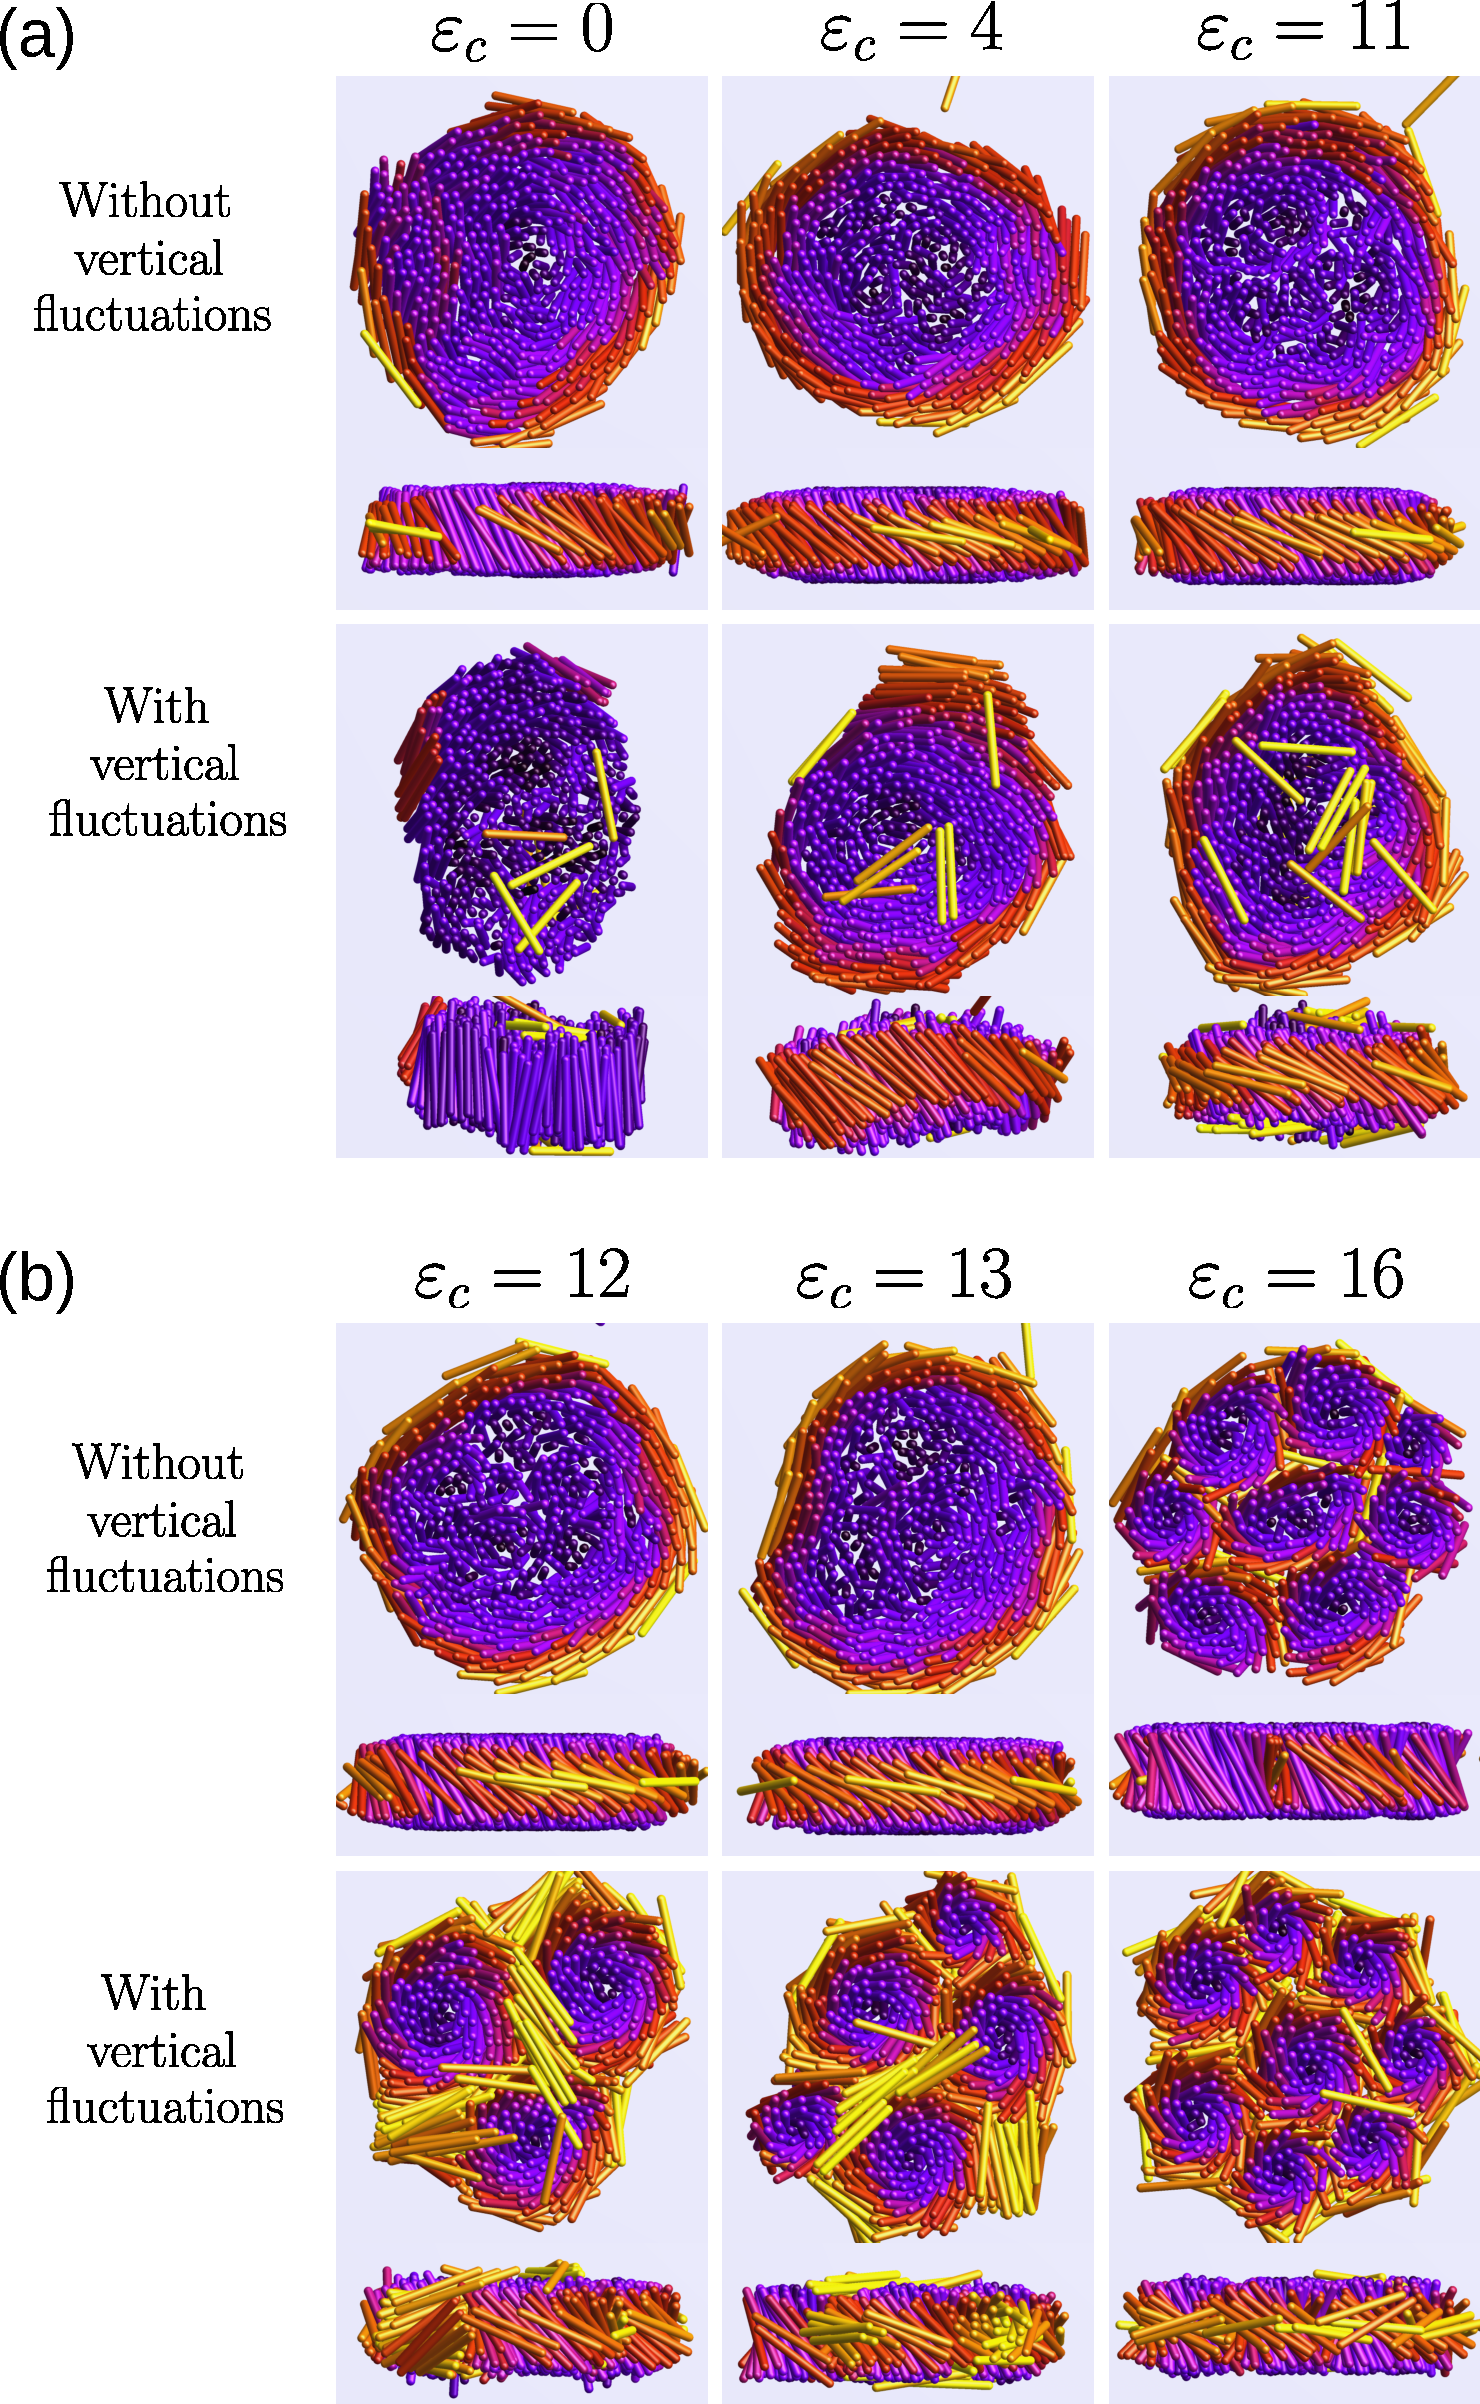
\includegraphics[width = .7\columnwidth]{figures/chapter-6/samples}
	\caption{Membrane-shaped tactoids of chiral rods mixed with non-adsorbing polymer formed in bulk (no confinement). For all runs, $\sigma = D$, chiral radius $d = 0.4D$, $\phi_{P}$ and $N = 500$. (a)-(b) $\varepsilon_{c}=0.5k_BT$, (c)-(d) $\varepsilon_{c}=1k_BT$ Top panels (a),(c) correspond to a top view of the system, bottom panels (b), (d) correspond to a side view with angle indicated by an arrow at the top panels.}
	\label{samples}
\end{figure}

\begin{figure}
	\includegraphics[width = 0.4 \columnwidth]{figures/chapter-6/impl_depletion_effect}
	\caption{ Spindle-shaped tactoids of achiral rods ($\varepsilon_{c}=0$) mixed with non-adsorbing polymer ($\sigma = 2D$) \red{in strong planar confinement ($h = L+D$)}. a) Weak depletion  (very low polymer packing fraction) and $N=500$. b) Strong depletion; $\phi_{P} =3$, $N=500$. c) Strong depletion; $\phi_{P} =3$, $N=1000$. The difference between the shapes between (b) and (c) is explained in \cite{kuhnhold2022structure} for 3-dimensional tactoids: larger nematic droplets tend to be less elongated. The structure in panel (b) is used as an initial configuration in the samples shown in \fig{samples}}
	\label{notwist}
\end{figure}



\clearpage % Nematic droplets
\input{chapters/chapter-7} % Conclusions




%%%%%%%%%%%%%%%%%%%%%%%%%%%%%%%%%%%%%%%%%%
% bib && appendices
%%%%%%%%%%%%%%%%%%%%%%%%%%%%%%%%%%%%%%%%%%
\backmatter
\appendix
\cleardoublepage
\addcontentsline{toc}{part}{Appendices}
\input{chapters/appendix}

\bibliography{bib/pub}
\addcontentsline{toc}{part}{Bibliography}



\includepdf[pages={2}]{coverpage/TORRES_coverpage.pdf}
\end{document}
